\documentclass[a4paper, 12pt]{book}
\usepackage[a4paper, left=2.5cm, right=2.5cm, top=3cm, bottom=3cm]{geometry}
%\usepackage[a4paper]{geometry}
\usepackage{times}
\usepackage{color}
\usepackage[usenames,dvipsnames,svgnames,table]{xcolor}
\usepackage[utf8]{inputenc}
\usepackage[textwidth=2cm]{todonotes}
\usepackage[hyphens]{url}
\usepackage[english]{babel}
%\usepackage[dvipdfm]{graphicx}
\usepackage{float}
\usepackage{placeins}
\usepackage[nottoc, notlot, notlof, notindex]{tocbibind}
\usepackage{latexsym}  %% Logo LaTeX
\usepackage{graphicx}
\usepackage{multirow}
\usepackage[colorlinks,bookmarksopen]{hyperref}
\usepackage{booktabs}
\usepackage{etoolbox}
\makeatletter
\preto{\@verbatim}{\topsep=0pt \partopsep=0pt }
\makeatother

%\usepackage[svgnames]{xcolor}

\restylefloat{table}
\restylefloat{figure}

%% PDF metadata
\hypersetup{
  pdftitle={The OpenDaylight Open Source Project},
  pdfauthor={Sergio Najib Arroutbi Braojos},
  pdfcreator={Master on Libre Software (URJC), Universidad Rey Juan Carlos},
  pdfproducer=PDFLaTeX,
  pdfsubject={Libre Software},
  %%% change colors to darker ones (for printing in B/W)
  linkcolor=Sepia,
  citecolor=OliveGreen,
  filecolor=violet,
  urlcolor=blue
}
%%

% Alter some LaTeX defaults for better treatment of figures:
    % See p.105 of "TeX Unbound" for suggested values.
    % See pp. 199-200 of Lamport's "LaTeX" book for details.
    %   General parameters, for ALL pages:
    \renewcommand{\topfraction}{0.9}	% max fraction of floats at top
    \renewcommand{\bottomfraction}{0.8}	% max fraction of floats at bottom
    %   Parameters for TEXT pages (not float pages):
    \setcounter{topnumber}{2}
    \setcounter{bottomnumber}{2}
    \setcounter{totalnumber}{4}     % 2 may work better
    \setcounter{dbltopnumber}{2}    % for 2-column pages
    \renewcommand{\dbltopfraction}{0.9}	% fit big float above 2-col. text
    \renewcommand{\textfraction}{0.07}	% allow minimal text w. figs
    %   Parameters for FLOAT pages (not text pages):
    \renewcommand{\floatpagefraction}{0.7}	% require fuller float pages
	% N.B.: floatpagefraction MUST be less than topfraction !!
    \renewcommand{\dblfloatpagefraction}{0.7}	% require fuller float pages

\frenchspacing

\title{The OpenDaylight Open Source Project}
\author{Sergio Najib Arroutbi Braojos}

\newcounter{appendixsection}
\setcounter{appendixsection}{0}

\renewcommand{\baselinestretch}{1.5}

\begin{document}

\newcommand\Sec[1]{%
   \leavevmode\par
   \stepcounter{appendixsection}
   \noindent
   \textbf{Section \theappendixsection. #1}.}

%\renewcommand{\refname}{Bibliography}
\renewcommand{\appendixname}{Appendix}

%%%%%%%%%%%%% COVER %%%%%%%%%%%%%%%%
\begin{titlepage}
\begin{center}
\begin{tabular}[c]{c c}
%
\includegraphics[bb=0 0 194 352, scale=0.25]{logo} &

\includegraphics[scale=0.25]{img/logo.png} &
\begin{tabular}[b]{l}
\Huge
\textsf{UNIVERSIDAD} \\
\Huge
\textsf{REY JUAN CARLOS} \\
\end{tabular}
\\
\end{tabular}

\vspace{3cm}

\Large
Máster Universitario en Software Libre

\vspace{0.4cm}

\large
Curso Académico 2014/2015

\vspace{0.8cm}

Proyecto Fin de Máster

\vspace{2.5cm}

\LARGE
The OpenDaylight Open Source Project

\vspace{4cm}

\large
Autor: Sergio Najib Arroutbi Braojos \\
Tutor: Dr. Gregorio Robles
\end{center}
\end{titlepage}
%%%%%%%%%%%%%%%%%%%%%%%%%%%%%%%%%%%%%%
\newpage
~

\newpage
~
\thispagestyle{empty}
\vspace{3cm}
\begin{flushright}
\textbf{\textit{Agradecimientos}} \\
\textit{A mi familia y a mi pareja, por su apoyo incondicional\\
Al equipo de Libresoft de la Universidad Rey Juan Carlos,
por su afán en enseñar el qué y el porqué del Software Libre}
\vspace{2cm}

\textbf{\textit{Dedicatoria}} \\
\textit{Para todos aquellos que hacen posible el fenómeno del Software Libre}
\end{flushright}

\newpage
~


\newpage
~
\thispagestyle{empty}
\vspace{12cm}
\begin{flushright}

(C) 2014 Sergio Najib Arroutbi Braojos. Some rights reserved.

This document is distributed under the Creative Commons
Attribution-ShareAlike 3.0 license,
available in \url{http://creativecommons.org/licenses/by-sa/3.0/}

Source files for this document are available at
\url{http://github.com/MFP/opendaylight.tex}
\end{flushright}

\newpage
~

\tableofcontents

\listoffigures

\listoftables

%%%%%%%%%%%%%%%%%%%%%%%%%%%%%%%%%%%%%%

\chapter*{Summary}
\markboth{SUMMARY}{SUMMARY}
\label{chap:summary}

The main goal of this work is to perform a deep analysis about the OpenDaylight Open Source Project. This collaborative project, hosted by the Linx Foundation, has been created in order to achieve one mission: \textbf{Develop an Open Source Programmable Networking Platform}.\\
\\
In this document, a detailed study of the different Open Source aspects having to do with project of this type of characteristics will be analyzed. Examples of this aspects, are, for instance, the licensing mechanism adopted by the project, the community behind the project, descriptive statistics about the project, the economic aspects around the project, as well as the technical state of the proyect and how OpenDaylight has progressed from its foundation date.


\chapter*{Resumen}
\markboth{RESUMEN}{RESUMEN}
\label{chap:resumen}

El principal objetivo de este trabajo es realizar un análisis detallado del projecto de código abierto OpenDaylight. Este proyecto colaborativo, perteneciente a la Linux Foundation, ha sido creado para una misión principal: \textbf{Desarrollar una plataforma de Código Abierto para Redes Programables}.\\
\\
En este documento, un estudio pormenorizado de los distintos aspectos asociados al Código Abierto asociados para un proyecto de estas características serán analizados. Un ejemplo de los aspectos a estudiar será el mecanismo de sistema de licencias, la comunidad que reside detrás del proyecto, estadísticas descriptivas del proyecto, los aspectos económicos, si los hubiera, alrededor del proyecto, así como el estado a nivel técnico o cómo ha evolucionado OpenDaylight desde la fecha de su fundación.

%%%%%%%%%%%%%%%%%%%%%%%%%%%%%%%%%%%%%%

\chapter{Introduction}
\label{chap:introduction}

\section{Terminology}
\label{sec:terminology}

\subsection{Open Source Programmable Networking}
\label{subsec:freesoftware}
In the same way Cloud Computing means a revolution in Computer Science, where computing resources are considered as flexible facilities to provide different kind of services, Networking is evolving in the same way. Networks hardware is considered to be a resource that is flexible and easily programmable in order to adapt to the specific Networking necessities. \textbf{SDN}~\cite{OpenNetworkingSDNDefinition} (Software Defined Networking) and \textbf{NFV}~\cite{ETSINFVDefinition} (Network Functions Virtualization) technologies have been strongly brougth to foreground in Networking Science, in order to provide,on the one hand, management of the network services through abstraction of lower level functionality and characteristics, and, on the other hand to provide a network architecture virtualization technologies to simulate nodes exisiting on a network.\\
\\
Around these technologies, The OpenDaylight Open Source Project, hosted by the Linux Foundation, has appeared to provide mechanisms not only to use previous described technology, but also to guarantee all the potential users of this technology the Freedoms that Open Source means, i.e.:
\begin{itemize}
 \item Freedom to use the program, for any purpose
 \item Freedom to study and adapt the programs (modify)
 \item Freedom to distribute the program to others
 \item Freedom to distribute to others the modified versions of the program
\end{itemize}
Analyzing The OpenDaylight Open Source Project is a good oportunity to investigate, on the one hand, an incipient technology and how an also incipient Open Source Project can influence not only on that technology, but also on the different aspects around a technology, as people involved on the technology develeopment (Community), the impact on the Economic aspects around the technology, and, above all, the aspects that Open Source itself supposes for this kind of projects.

\section{About this document}
\label{sec:about}

\subsection{Document structure}

In order to provide a detailed analysis of The OpenDaylight Open Source Project, this work contains different chapters to describe the different important aspects aroud the project from an Open Source perspective:

\begin{table}[H]
\footnotesize
\begin{center}
\begin{tabular}{|p{5cm}|p{10cm}|}
\hline
\textbf{Chapter Name} & \textbf{Description} \\ \hline
Introduction & A complete introductory overview of The OpenDaylight Open Source Project \\
\hline
OpenDaylight Economic Aspects & Detailed study of economic aspects around the project \\
\hline
OpenDaylight Legal Aspects & Complete analysis of the license or licenses used in OpenDaylight and the different advantages and disadvantages of this kind of licensing scheme \\
\hline
OpenDaylight Governance and Community Management & Analysis of the community and its governance, its organization, communication channels, politics and mission \\
\hline
OpenDaylight Technical Aspects & Study of the technology behind the project and its scope \\
\hline
OpenDaylight Project Evaluation & Graphics and statistics around the OpenDaylight project, such as number of commiters, number of open/closed issues, mail lists statistics, activity and in general all statistics to perform an evaluation of the project from a statistical perspective \\
\hline
\end{tabular}
\end{center}
\caption{Document Structure}
\label{tab:documentstructure}
\end{table}

\subsection{Scope}
\label{subsec:scope}
This document is not entitled to perform a complete description of the different protocols and technologies that OpenDaylight uses in order to achieve the programmability network platform it pretends to provide. They will be smoothly analyzed in order to clarify how OpenDaylight works, but not all of the technologies will be described, and those described will not be done in deep.

Beyond the purely technical aspects, this work pretends to focus on analyzing OpenDaylight project from an Open Source perspective, analysing the pros and cons of Open Source, and the different aspects that an Open Source Project faces.

\subsection{Methodology}
\label{subsec:methodology}
Different tools and documentation have been used in order to perform this work. Docmentation used have been basically the different Web Pages available around The OpenDaylight Open Source Project~\cite{OpenDaylight}. A complete description of the documentation used will be provided in the Bibliography.

Regarding tools, apart from Web-Browsers used to navigate through the project documentation, the different metrics obtained around OpenDaylight project have been obtained through MetricsGrimoire~\cite{MetricsGrimoire}. In particular, among the tools existing on MetricsGrimoire, CVSanaly~\cite{CVSanaly}, Bicho~\cite{Bicho} and MailingListStats~\cite{MailStats} were used.\\
\\
Apart from that, SLOCCount~\cite{SLOCCount} tool has been used in order to detect the amount of lines of code that exist on the project, as well as the different programming languages used in the project implementation and its respective distribution inside the project.SLOCCount output has been processed with a text processing tool, \textbf{gawk}~\cite{GAWK}. Other utility, Python matplotlib~\cite{PyMatplotlib}, has been used to generate graphics on certain kind of metrics.

%%%%%%%%%%%%%%%%%%%%%%%%%%%%%%%%%%%%%%
\chapter{Goals and Objectives}
\label{chap:Goals}
\section{General Objectives}
\label{sec:genobj}

The general objectives of this work are, basically, on the one hand, acquiring knowledge, competence and skills around OpenDaylight, while, on the other hand, analysing the project from an Open Source perspective.

\section{Subobjectives}
\label{sec:subobj}

%%%%%%%%%%%%%%%%%%%%%%%%%%%%%%%%%%%%%%
In order to achieve the objectives this work pursues next operative objectives have been identified:

\begin{itemize}
\item{Acquire competence on OpenDaylight project}
\item{Analyze OpenDaylight project from an Open Source perspective}
\item{Extract the most significant statistics in OpenDaylight project to determine its state of the art}
\end{itemize}

\subsection{Acquire competence on OpenDaylight project}
\begin{itemize}
 \item Perform an overall description of the OpenDaylight project.
 \item Acquire competence on OpenDaylight documentation, and sinthesize the most important aspects of the project.
 \item Analyze the technical aspects of the project and determine its Ease of Use.
\end{itemize}

\subsection{Analyze OpenDaylight project from an Open Source perspective}
\begin{itemize}
 \item Analyze the licensing model followed by the project
 \item Study the economic aspects behind this project
 \item Determine the different aspects behind the project's community
\end{itemize}

\subsection{Statistics and measures of the OpenDaylight project}
\begin{itemize}
 \item Perform a complete measures compilation of the project
 \item Evaluate the State of the Art of the project based on its measures
\end{itemize}

\chapter{OpenDaylight: A first view}
\label{chap:odlfirstview}

\section{OpenDaylight Project}
\label{sec:odlintro}

OpenDaylight is a collaborative project, started in April 8, 2013~\cite{OpenDaylightAnnouncement}, and developed inside the Linux Foundation Collaborative Projects ecosystem. This fact is the first one to remark, due to the fact that, normally, projects under the Linux Foundation are supposed to have strong economic and infrastructure support, due to the following reasons:
\begin{itemize}
 \item \textbf{Linux Foundation} is one of the most profitable Open Source organizations, mostly due to the importance of its main project, \textbf{the Linux Kernel Project}. In 2012, The Linux Foundation obtained a \textbf{total revenue of \$17,123,662}, according to ~\cite{2012LinuxFoundationReport}. Among the collaborators of the Linux Foundation Collaborative Projects, next ones are to remark: ~\cite{LinuxFoundationCollaborativeProjects}
 \begin{enumerate}\itemsep0pt
  \item Cisco
  \item Google
  \item HP
  \item IBM
  \item Intel
  \item Qualcomm Innovation Center
  \item Samsung
  \item New York Stack Exchange Technologies
 \end{enumerate}
 \item \textbf{Collaborative Projects} under the Linux Foundation are only a few, in a more focused strategy compared to other organizations hosted in other organizations such as Mozilla Foundation, the Apache Software Foundation or the Free Software Foundation, that fund more projects. Examples of other projects hosted by the Linux Foundation Collaborative Projects are ~\cite{LinuxFoundationCollaborativeProjects}:
 \begin{enumerate}\itemsep0pt
  \item Allseen Alliance
  \item Code Aurora
  \item MeeGo
  \item OpenVirtualization Alliance
  \item The Bel Language
  \item OpenMama
  \item Tizen
  \item Xen Project
  \item Yocto Project
 \end{enumerate}
\end{itemize}
Being a Linux Foundation Collaborative Project, OpenDaylight is part of a technology that is booming in the last years, having to do with \textbf{SDN} and, to a lesser extent, with NFV, in particular in the Networking Industry. According to OpenDaylight project ~\cite{OpenDaylightTheProject}:
\begin{verbatim}
OpenDaylight is a community-led, open, industry-supported
framework, for accelerating adoption, fostering new innovation,
reducing risk and creating a more transparent approach to
Software-Defined Networking.
OpenDaylight is a Collaborative Project at The Linux Foundation.
It is structured using open source development best practices,
and is comprised of the leading organizations in the technology
industry.
\end{verbatim}
In particular, as stated in the ``About'' section of OpenDaylight project~\cite{OpenDaylightAbout}, the adoption of new technologies and pursuit of programmable networks has the potential to significantly improve levels of functionality, flexibility and adaptability of mainstream datacenter architectures.\\
\\
Leveraging this abstraction to its fullest requires some adaptation from the network perspective, as well as adaptation and evolution to a Software-Defined architecture. One of the most important architectural elements required to achieve this goal is SDN and NFV platform, to enable network control and programmability from a centralized point.\\
\\
SDN, and NFV to a lesser extent, are a hotbed of innovation nowadays, with a bunch of vendors bringing products and technologies to market. Ironically, the myriad options may prove counterproductive to SDN and NFV adoption. At this early stage of SDN and NFV adoption, the industry acknowledges the benefits of establishing an open, reference framework for programmability and control through an open source SDN and NFV solution.\\
\\
Such a framework maintains the flexibility and choice for organizations to deploy SDN and NFV as they still mitigates many of the risks of adopting early stage technologies and integrating with existing infrastructure investments.\\
\\
With OpenDaylight, a community with some of the most important companies involved in Computer Science, Virtualization and Networking Industry, has come together to fill this need through the combination of open community developers and open source code and project governance that guarantees an open, community decision making process on business and technical issues. \textbf{Establishing an open source project in this way is designed to help accelerate the development of technology available to users} and enable widespread adoption of SDN and create a solid foundation for NFV.\\
\\
OpenDaylight can be a \textbf{core component} within any SDN architecture, providing an open source SDN and NFV controller that enables users to reduce operational complexity, extend the life of their existing infrastructure hardware and enable new services and capabilities only available with SDN.\\
\\
Whether an organization is an enterprise IT provider, a network service provider or a Cloud services provider, it can begin taking advantage of SDN and NFV using a community-driven, open source controller framework available today.\\
\\
The first open source software release by the OpenDayLight Open Source Project is known as \textbf{``Hydrogen''}. This release, Hydrogen, is the first simultaneous release of OpenDaylight, delivering three different editions to help a wide array of users get up and running as quickly as possible. The three options available are a Base Edition, a Virtualization Edition and a Service Provider Edition, and all of them are already available for download.\\
\\
But, \textbf{how important is this project from the Neworking Technology Industry main companies perspective?}. A view to the main members board of the OpenDaylight project is a clear idea of the importance of this project from the industry perspective, as well as how strategic is this technology perceived from the most important market leaders from not only the Networking Market but also from Computer Science and Computing Virtualization Maret leaders.\\
\\
Among the \textbf{platinum members of the project}, next ones are noteworthy~\cite{OpenDaylightMembers}:
 \begin{itemize}\itemsep0pt
  \item Brocade
  \item Cisco
  \item Citrix
  \item Ericsson
  \item HP
  \item IBM
  \item Juniper Networks
  \item Microsoft
  \item RedHat
 \end{itemize}
Meanwhile, the \textbf{golden members of the project}, are:
\begin{itemize}\itemsep0pt
 \item NEC
 \item vmWare
\end{itemize}
Last, but not least, there is a huge number of members (more than 25) considered as \textbf{silver members of the project}. Among these members, some of the most important are:
\begin{itemize}\itemsep0pt
 \item Intel
 \item Oracle
 \item Dell
 \item Huawei
 \item Fujitsu
 \item Avaya
 \item H3C
 \item Plexxi
 \item Zte
 \item ... and many others
\end{itemize}
So, to summarize, The OpenDaylight Project is a collaborative open source project that aims to accelerate adoption of Software-Defined Networking (SDN) as well as Network Functions Virtualization (NFV) for a more transparent approach that fosters new innovation and reduces risk.\\
\\
As shown before, there is a huge and increasing interest in this kind of technology by the most important companies. Why this interest in these technologies? Why and how are they changing the market in this kind of industry? Why is there a so huge interest in SDN from the industry main actors?\\
\\
In next sections a quick view of these technologies is provided, as well as some indicators of how quick this kind of technology is increasing inside the networking market.

\section{SDN}
\label{sec:sdn}

\subsection{What is SDN?}
SDN technology  allows network administrators to manage network resources as network services through abstraction of lower level provided functionality, by the physical separation of the network control plane from the forwarding plane, and where a control plane controls several devices~\cite{OpenNetworkingSDNDefinition}.\\
\\
Software-Defined Networking (SDN) has appeared as a dynamic, manageable, cost-effective, and adaptable emerging architecture, ideal for the high-bandwidth, dynamic nature of today's applications.\\
\\
This architecture decouples the network control and forwarding functions, enabling the first one to become directly programmable and the underlying infrastructure to be abstracted for applications and network services.\\
\\
Related to this, The OpenFlow™ protocol appears as a foundational element for building SDN solutions.

\begin{center}
 \begin{figure}[H]
 \begin{center}
   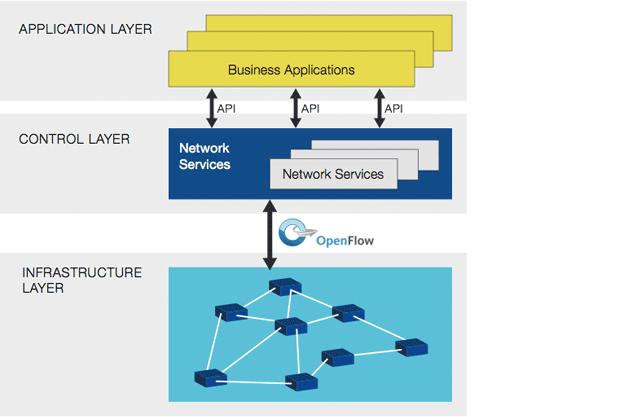
\includegraphics[width=20cm]{img/sdn-3layers.png}
   \caption{SDN 3 Layer Architecture}
   \label{fig:sdn3layer}
 \end{center}
 \end{figure}
\end{center}

SDN architecture is characterized by the following aspects:
\begin{itemize}
\item{\textbf{Open standards-based and vendor-neutral}}: Being implemented through open standards, SDN simplifies network design and operation. Instructions are provided by SDN controllers, which follow a particular set of open protocols and devices, instead of multiple, vendor-specific devices and protocols.
\item{\textbf{Directly programmable}}: Network control plane is directly programmable. This aspect is possible due to the fact that control planeis decoupled from forwarding plane.
\item{\textbf{Agile}}: Abstracting control from forwarding plane lets network administrators dynamically adjust network-wide traffic flow to meet particular needs of the network at each particular moment.
\item{\textbf{Centrally managed}}: Network intelligence is centralized in software-based SDN controllers. This kind of elements maintain a global view of the network topology. Network itself appears to applications and policy engines as a single, logical switch.
\item{\textbf{Programmatically configured}}: Network managers can configure, manage, secure, and optimize network resources through SDN very quickly via dynamic, automated SDN programs, which can be written themselves because the programs do not depend on proprietary software.
\end{itemize}
Previous detailed aspects make SDN technology to be one of the most recently boosting technologies, together with Cloud Computing and Big Data. Indeed, the increasing interests in all of them has also to do with the fact that all these technologies, together with Virtualization, are necessary linked between them.\\
\\
Next section shows how the market has increased in the last years, together with the big expectations that SDN tecnhology is supposed to have in the next years.

\subsection{SDN: Market share and expectations}
\label{subsec:sdn_marketshare}

SDN is considered a boosting technology. In year 2013, the service-provider SDN market —hardware and software combined — was about \textbf{\$840 million in 2013} and is considered to grow to \textbf{\$15.6 billion in 2018}, according to a report released by ACG Research~\cite{SDN2018expectations00}.\\
\\
In this research, numbers don’t include the enterprise market, and apply only to service providers, including large-data-center owners such as Google and the big data centers of carriers such as NTT or AT\&T.\\
\\
Here’s how ACG’s 2018 forecast breaks down into the different sub-markets taking into account the different main areas of SDN deployment:

\begin{table}[H]
\footnotesize
\begin{center}
\begin{tabular}{|l|l|l|}
\hline
\textbf{SDN Submarket} & \textbf{Market expectation} \\ \hline
Data center	& \$3.3 billion \\ \hline
IP services	& \$4.2 billion \\ \hline
Metro networks &	\$4.3 billion \\ \hline
Core networks & \$3.8 billion  \\ \hline
\end{tabular}
\end{center}
\caption{SDN 2018 Sub-Market Expectations}
\label{tab:2018submarketexpectations}
\end{table}
The numbers reflect only “live” SDN deployments, i.e.: cases where service providers would use the technology, and not just installing it for future use.\\
\\
However, it must be remarked that expectations are even higher considering other reports. By mid 2013, market considered for year 2013 was about \$1.5 billion, and expectations for year 2018 was about \$35.5 billion according to a research by SDNCentral~\cite{SDN2018expectations01}.

\begin{center}
 \begin{figure}[H]
 \begin{center}
   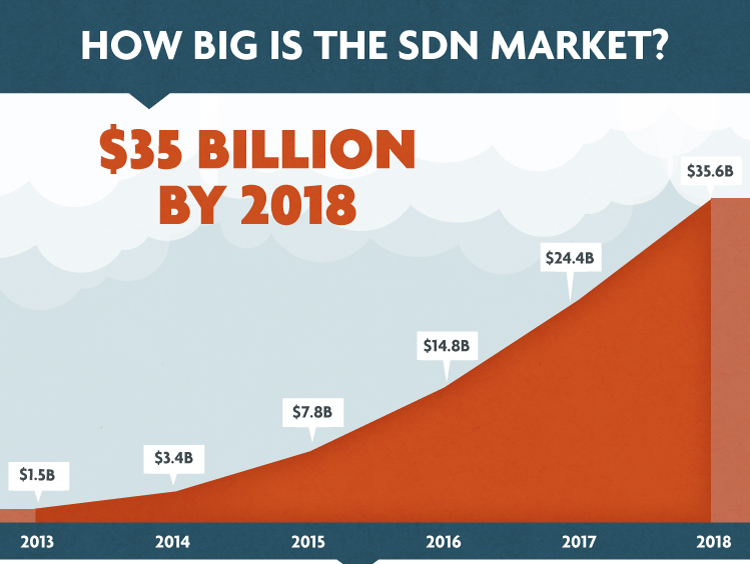
\includegraphics[width=15cm]{img/sdn_estimations_2018.png}
   \caption{SDN Market: 2018 SDNCentral estimations}
   \label{fig:sdn2018estimations}
 \end{center}
 \end{figure}
\end{center}

This last analysis and infographics doesn’t compare directly with previous one, as it wasn’t limited to service providers, and included SDN-ready equipment, sales that represent customers preparing for SDN even if they wouldn’t be using it immediately.\\
\\
Analyzing the data of this last report, a number of key takeaways must be highlighted:
\begin{enumerate}\itemsep0pt
 \item{The software-defined networking SDN market is expected to surpass \$35 billion in 2018}.
 \item{Adoption of SDN technology has accelerated in recent years from sales of \$10 million in 2007 to \$252 million in 2012}.
 \item{The emergence of the software-defined networking market is supported by growth in venture capital investment in SDN-focused companies}. Venture capital funding of SDN-related companies rose from \$10 million in 2007 to \$454 million in 2012.
\end{enumerate}

According to this report, the main three areas driving the rise in SDN are:
\begin{enumerate}\itemsep0pt
\item{Cloud Computing}
\item{Big Data}
\item{Mobility}
\end{enumerate}
Apart from pure SDN Market numbers, there are other aspects to consider. For example, the VC(Venture Capital) investment has grown, according to this report, from \$10 million in 2007 to \$454million in 2012.\\
\\
This report also considers that Networking Industry spending Percentage on SDN will rise from 2\% in 2013 to 40\% in 2014, with more than 220 companies by mid 2013, compared to the zero existing in 2009.\\
\\
Last, but not least, it must be remarked that up to more than \$1.5 billion has been invested in acquisitions of SDN related companies up to 2013, including the most remarkable one, the acquisition of Nicira Inc. by VMWare by July 2012, for approximately \$1.05 billion in cash plus approximately \$210 million of assumed unvested equity awards~\cite{VMWareAcquireNicira}.\\
\\
Far from giving a very detailed information on SDN market, this section has shown through all the numbers above how important is the SDN market and how important could be an Open Source Software Project such as OpenDaylight, which is in the end a key component in SDN deployment.

\section{NFV}
\label{sec:nfv}

Network Functions Virtualisation is a concept directly tied to Network Operators, as, normally, therir networks consist of a large and increasing variety of proprietary hardware and software applications that implement different functionality.\\
\\
To launch a new service on a Network Operator usually requires yet another different kind of hardware, meaning finding the space and power to accommodate these new equipment. As time goes by and Network Operator infrastructure grows, adding new appliances becoms more difficult, by the increasing costs of energy, capital investment challenges and, of course the rarity of skills necessary to design, integrate and operate these new equipment.\\
\\
Apart from that, end of life for hardware-based appliances is reached rapidly, requiring much of the integration and deploy cycle to be repeated with no revenue benefit in most of the cases. Besides this, hardware lifecycles are becoming shorter, due to the fact that technology and services innovation accelerates quicker up on time.

\subsection{What is NFV?}

As defined by \textbf{ETSI} in~\cite{ETSINFVDefinition} defines \textbf{Network Functions Virtualisation} as follows:
\begin{verbatim}
Network Functions Virtualisation aims to transform
the way that network operators architect
networks by evolving standard IT virtualisation
technology to consolidate many network equipment
types onto industry standard high volume servers,
switches and storage, which could be located in
Datacentres, Network Nodes and in the end user
premises.
\end{verbatim}
What NFV aims to get is, basically, homogenize the hardware of a Network Operator to basically three kind of standard generic use hardware. In particular, by the use of \textbf{High Volume Servers}, \textbf{High Volume Storage} and \textbf{High Volume Ethernet Switches}. Accomplishing this homogenization involves the implementation of \textbf{Network Functions} in software. This Network Functions must run on a range of industry standard server hardware, and can be moved to, or instantiated in, various locations in the network as required, without the need for installation of new equipment, at least, from a functional perspective.\\
\\
In the end, for Network Operators, NFV means migration of the different hardware specific nodes implementing different functionalities, such as DPI (Deep Packet Inspection), Firewalls, CDN (Content Delivery Network), Radio Access Network Nodes, Message Router, Carrier Grade NAT and/or any other network specfic functionality, which involve \textbf{Fragmented non-commodity hardware}, to Network Functions (also known as \textbf{Virtual Appliances}) running on previously defined Standard High Volume hardware.

\begin{center}
 \begin{figure}[H]
 \begin{center}
   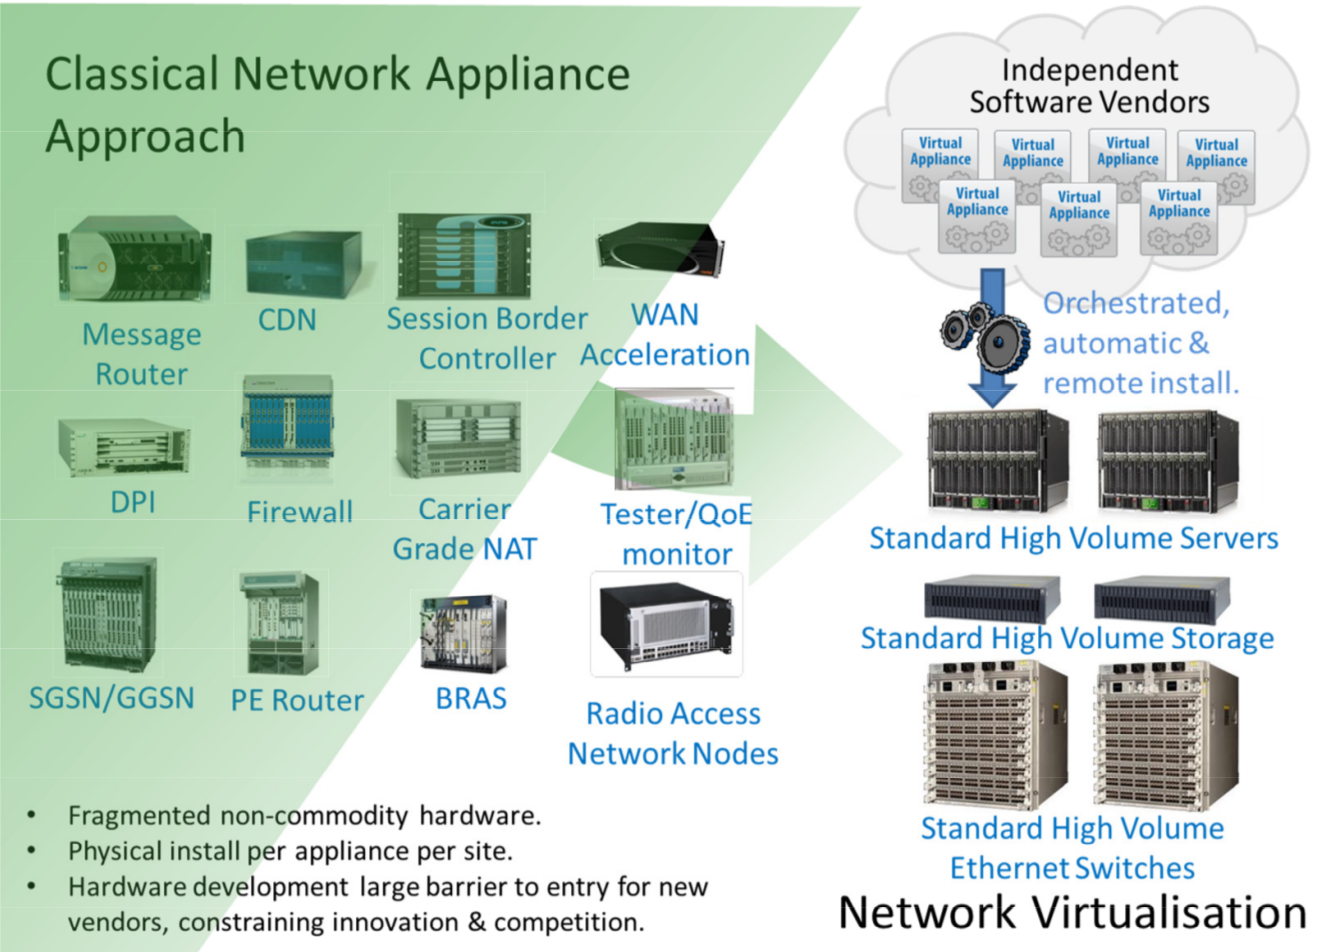
\includegraphics[width=15cm]{img/nfv-etsi-01.png}
   \caption{Vision of Network Functions Virtualisation}
   \label{fig:nfv_vision}
 \end{center}
 \end{figure}
\end{center}

\subsection{SDN/NFV relationship}

Network Functions Virtualisation is highly complementary to Software Defined Networking (SDN), as recognized by \textbf{ETSI} in~\cite{ETSINFVDefinition}. However NFV is not dependent on SDN (or vice-versa). NFV can be implemented without a SDN being required, although the \textbf{both solutions can be combined and potentially greater value accrued}.\\
\\
Network Functions Virtualisation goals can be achieved using non-SDN mechanisms, relying on the techniques currently in use in many operators. But approaches relying on the separation of the control and data forwarding planes as proposed by SDN can enhance performance, simplify compatibility with existing deployments, and facilitate operation and maintenance procedures.\\
\\
Network Functions Virtualisation is able to support SDN by providing the infrastructure upon which the SDN software can be run. Furthermore, Network Functions Virtualisation aligns closely with the SDN objectives to use commodity servers and switches.

\begin{center}
 \begin{figure}[H]
 \begin{center}
   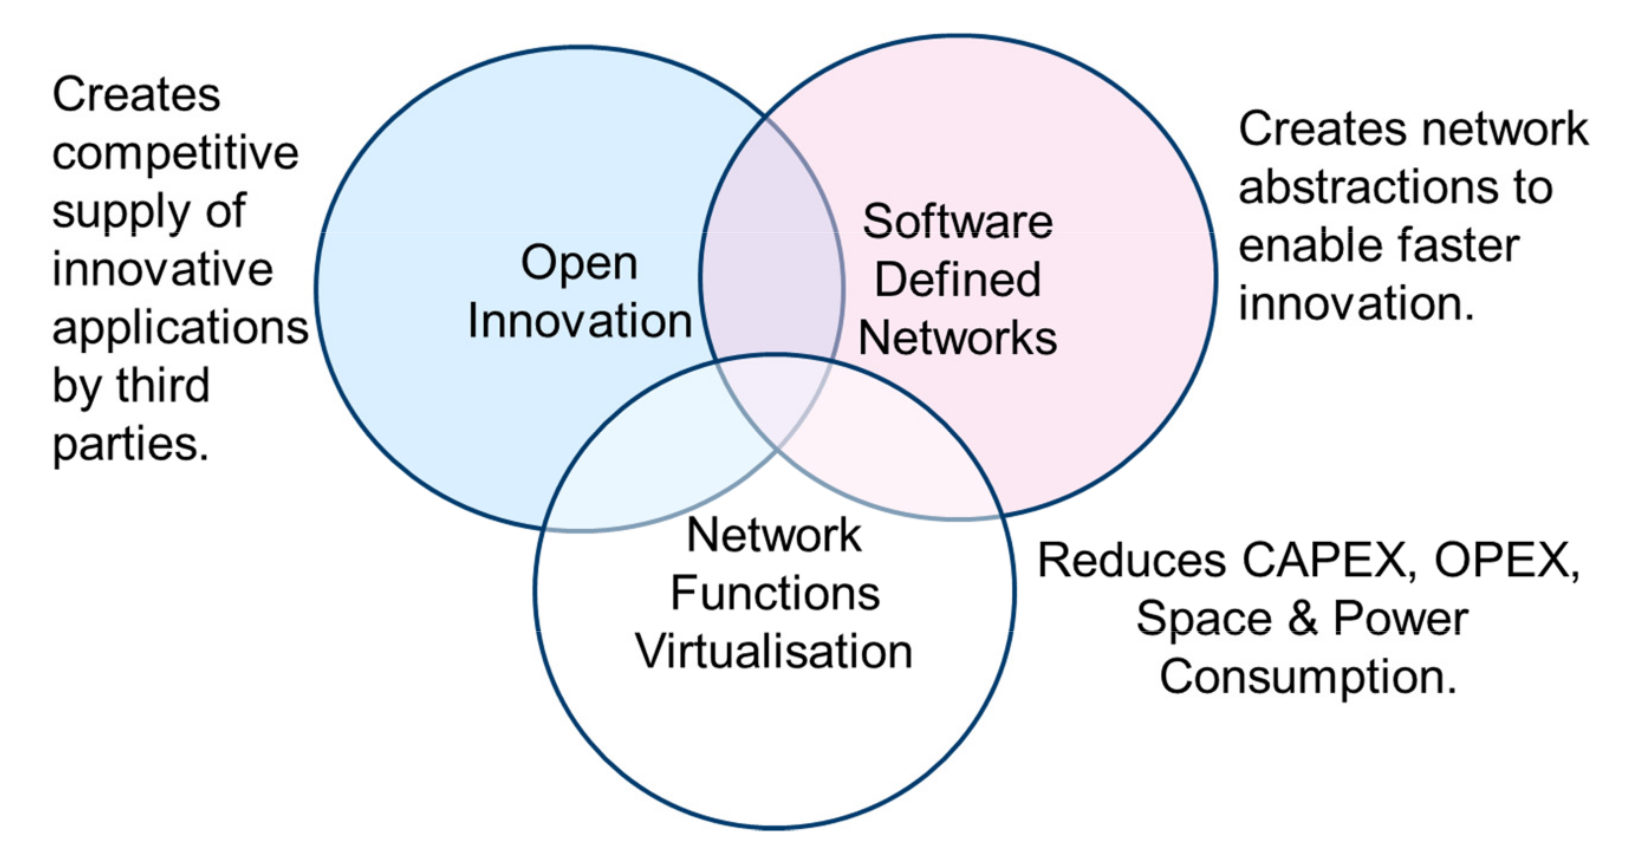
\includegraphics[width=15cm]{img/sdn-nfv-relationship-00.png}
   \caption{Network Functions Virtualisation relationship with SDN}
   \label{fig:nfv_sdn_relationship}
 \end{center}
 \end{figure}
\end{center}
ETSI intends to work closely with organisations progressing work on SDN such as the Open Networking Foundation (ONF) whose work is specifically taken into account by SDN to achieve common goals.

\subsection{NFV benefits}

Taking into account previous sections, where NFV concept has been detailed, an analysis of the main benefits of the migration of the Network Operators to this kind of infrastructure based on Virtual Appliances running on common High Volume Hardware. ETSI~\cite{ETSINFVDefinition} defines next \textbf{benefits} for a Network Operator taking into account migration to Network Functions Virtualisation:

\begin{itemize}\itemsep0pt
 \item{\textbf{Reduced equipment cost}}. Basically, by exploiting the economies of scale of the IT industry.
 \item{\textbf{Increased velocity of Time to Market}}. By minimising the network operator cycle of innovation.
 \item{\textbf{Reduction of development costs and time to market}}. Motivated by a more efficient test and integration, and the possibility of running production, test and reference facilities on the same infrastructure.
 \item{\textbf{More innovation due to openness}}. Motivated by Open Virtual Appliance market where small players and academia can bring new services.
 \item{\textbf{Optimizing network configuration and/or topology}}. This optimization can be performed in near real time based on the actual traffic/mobility patterns and service demand.
 \item{\textbf{Reduced energy consumption}}. By exploiting power management features in standard servers and storage hardware.
 \item{\textbf{Improved Operational Efficiency}}. Taking advantage of the uniformity of the physical network platform:
 \begin{itemize}\itemsep0pt
    \item{IT orchestration mechanisms provide automated installation}.
    \item{Eliminating the need for application-specific hardware}. The skills base across the industry for operating standard high volume IT servers is much larger and less fragmented.
    \item{Reduction in variety of equipment for planning and provisioning}.
    \item{Option to temporarily repair failures by automated re-configuration}.
    \item{The potential to gain more efficiency between IT and Network Operations}.
    \item{The potential to support in-service software upgrade}.
 \end{itemize}
\end{itemize}
On this chapter, a first introduction to the \textbf{OpenDaylight Open Source Project} has been presented. Apart from that, main technologies involved in this project, \textbf{SDN} and \textbf{NVF} have been introduced as well. On next sections, it will be studied in depth other aspects of the project, focusing on those areas having to do with Open Source nature of the project.

\chapter{OpenDaylight: Economic Aspects}
\label{chap:odleconomic}

Economic issues around Open Source software are always there. It is important to separate Open Source software itself from its usual ``costless'' nature. Free Sotware itself has not helped to this separation, as free refers to the ``Freedom'' aspect, not to the costless aspect. Richard Stallman is the one how has most times clarified this:
\begin{verbatim}

To understand the concept, you should think of "free" as in
"free speech" not as in "free beer".

\end{verbatim}
This chapter will analyze the economic aspects after OpenDaylight Open Source project. First of all, the SDN and NVF market will be analyzed. Although some data on the market expectations that this technology aroused ~\ref{tab:2018submarketexpectations} on the first days. However, a more detailed analysis of the current state of SDN/NFV market will be performed to identify the accomplishment of the expectations.\\
\\
Apart from that, it is important to identify that SDN/NVF technologies, as incipient technologies, could mean new business models for selling companies, as well as new cost saving methods for network operators, as was justified in ~\ref{sec:nfv}. Both aspects will be analyzed on this chapter as well.\\
\\
Last, but not least, it is important to focus on the OpenDaylight project. Why has this Open Source project been founded? Was it done as a way of altruism? Or it was rather to respond to a certain particular need on the Networking industry? Last section of this chapter analyses those facts that could mean the foundation of OpenDaylight project, as well as reasons to go Open Source.

\section{SDN and NFV: A new market}
\label{sec:odlnewmarket}

As remarked in previous section~\ref{subsec:sdn_marrketshare}, by 2013 there were big expectations in networking industry around SDN/NVF technologies. Some optimistic reports predicted a market expectations for year 2018 about \$35.5 billion, while others were more cautious and estimated \$15.6 billion by that same year.\\
\\
It is usually common that real market do not follow market spectations for those cases where a technology is on its incipient state. The \textbf{hype cycle}, a branded graphical theory developed by IT research firm Gartner, do already consider that \textbf{peak of inflated expectations}.
\begin{center}
 \begin{figure}[H]
 \begin{center}
   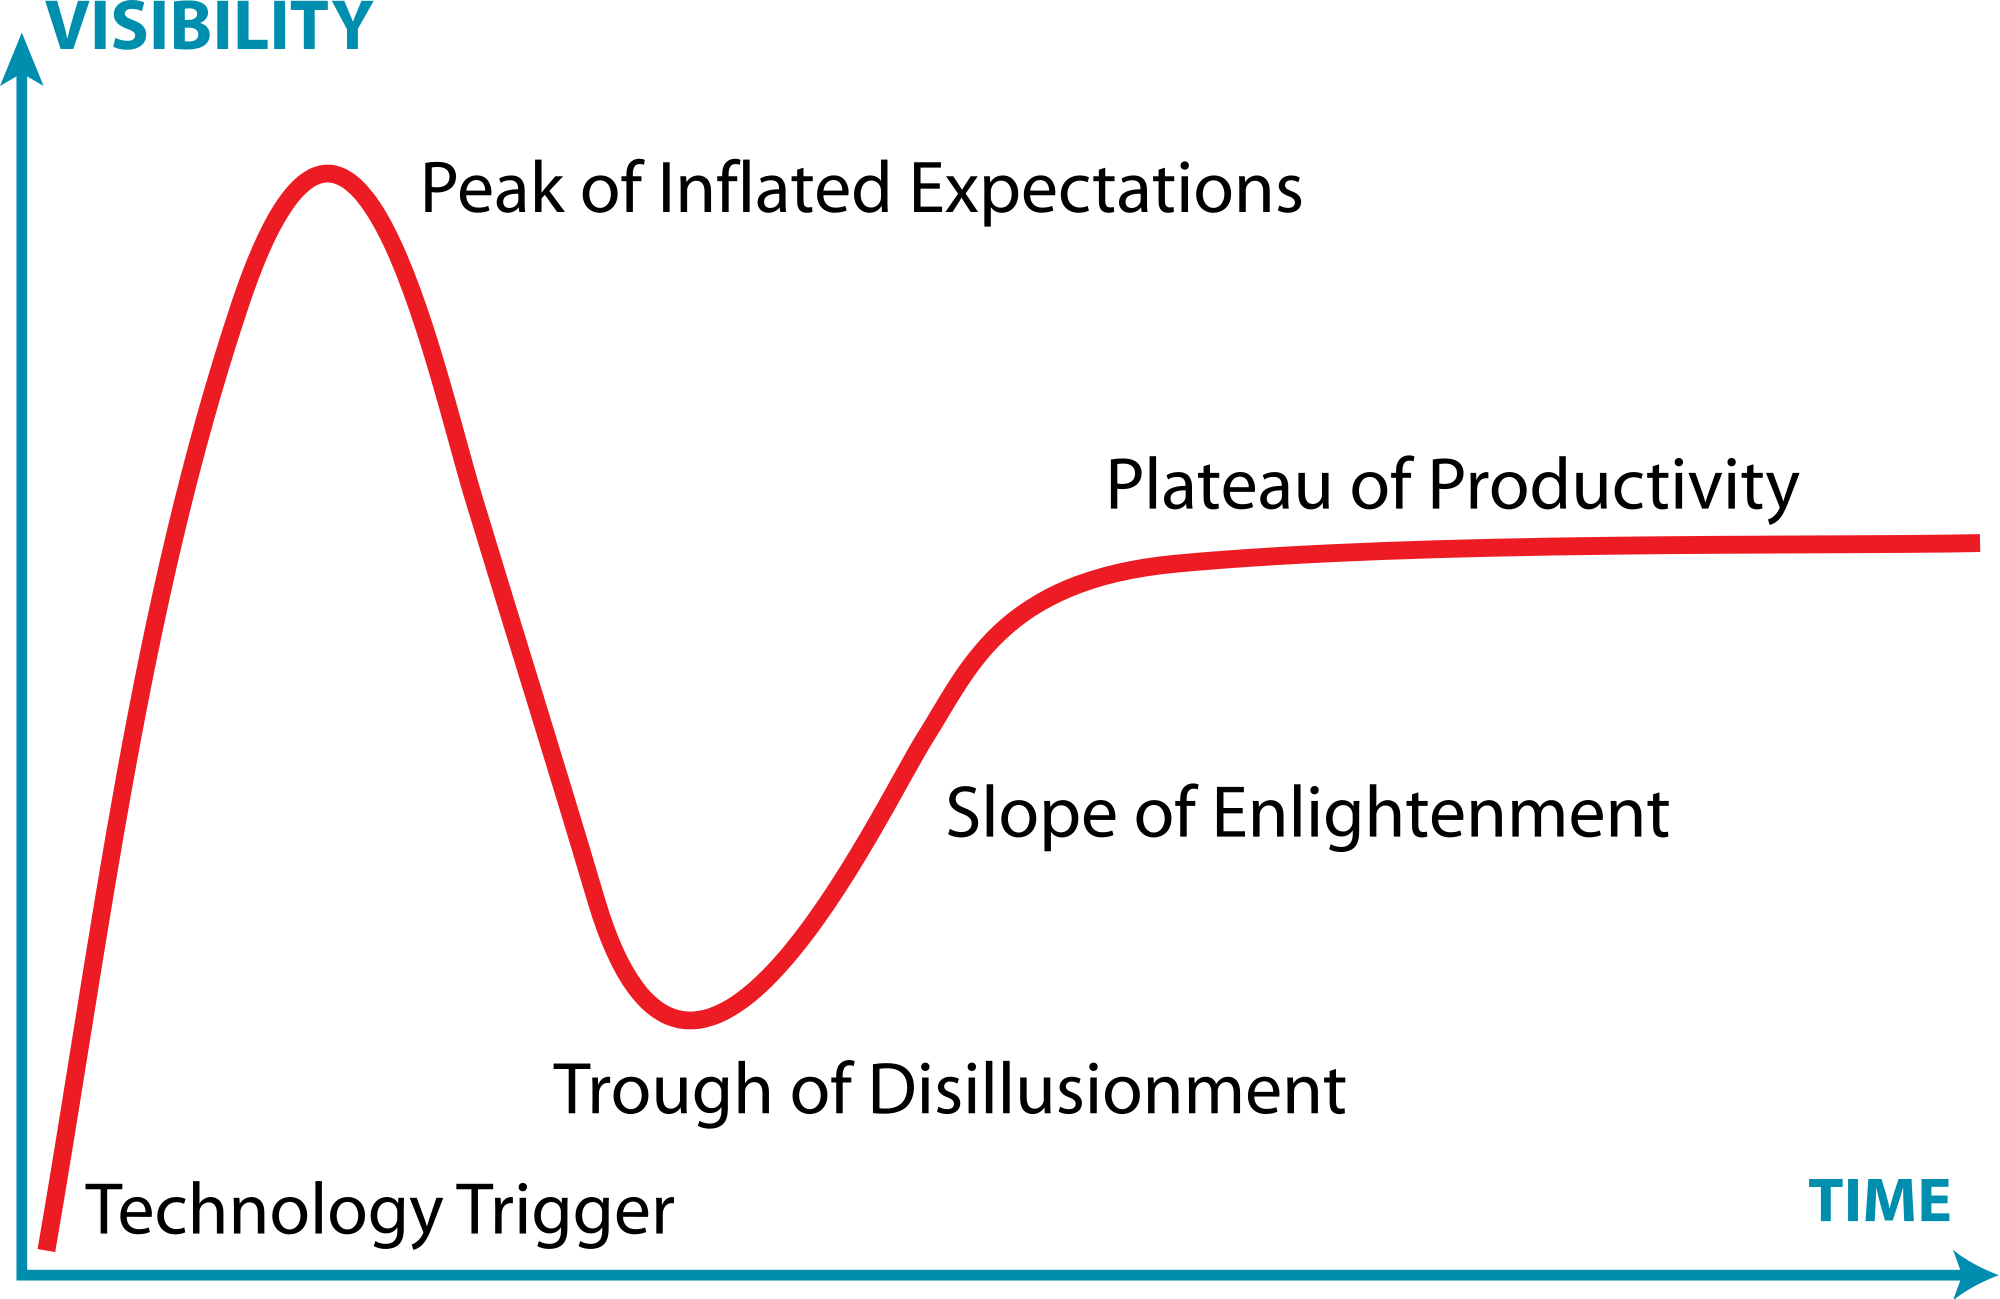
\includegraphics[width=15cm]{img/hype-cycle-00.png}
   \caption{Gartner Hype Cycle}
   \label{fig:gartner_hype_cyle}
 \end{center}
 \end{figure}
\end{center}

This cycle~\cite{HypeCycle}, which tries to represent the maturity, adoption and social application of specific technologies, fits well to describe what is going on in SDN/NFV technology life cycle. From Hype Cycle's persective, the life cycle of a technology has five different phases:

\begin{enumerate}\itemsep0pt
\item{\textbf{Technology Trigger}}. A potential technology breakthrough arises interest.
\item{\textbf{Peak of Inflated Expectations}}. Early publicity produces a number of success stories.
\item{\textbf{Through of Disillusionment}}. Interest wanes as experiments and implementations fail to deliver.
\item{\textbf{Slope of Enlightment}}. More instances of how the technology can benefit the industry start to become true.
\item{\textbf{Plateau of Productivity}}. Mainstream adoption starts to take off.
\end{enumerate}
SDN/NFV technologies seem to have crossed the Peak of Inflated Expectation and are starting down that part of the Gartner Hype Cycle~\cite{SDNandNFVHypeCycle}. Second thoughts are starting to be present when talking about these technologies, where some disappointing facts have started to appear:
\begin{itemize}\itemsep0pt
\item{\textbf{NVF seem to not going to cut for high performance applications}}. NFV seems to have some hard problems related to the ``state'' IP networks own. NFV applications must deal with communications and therefore contain a fair amount of session state. This state must be accessed quickly to maintain performance, something which seems not easy in NFV architecture.
\item{\textbf{No impressive SDN/NFV IPOs companies have been performed}}. After initial IPOs around Nicira or Contrail from VMWare and Juniper respectively, it seems no big action regarding companies acquisitions exist. This is another measure of how this market is losing expectations.
\item{\textbf{SDN seems for the near future to be confined to the data center}}. Existing Internet Service Providers (ISPs) and Enterprise Networks, although evaluating SDN's impacts, are not defining transition plans with confidence.
\item{\textbf{Market sales are far from expectations}}. Some recent reports, such as the IDC~\cite{SDNMarket20142018IDC} one, are predicting sales of \$960M in 2014, which is far from the \$3.4B predicted in some of the most optimistic reports.
\end{itemize}
\textbf{SDN/NFV technologies are, in turn, suffering the perception of being a complicated technology}. In a survey performed to more than 100 IT professionals by Pica8~\cite{Pica8Survey}, the perception of more than \textbf{50\% of the professionals} was that \textbf{have no time or skills today to build the stack themselves}. Meanwhile, \textbf{20\% of the professionals} thought that \textbf{want an open platform, but they still need help selecting the pieces for their scenarios}.\\
\\
Together with all previous statements, there is a particular problem with SDN today, which is relate to the concept of adopting a new technology. In the end, \textbf{the challenge is that existing hardware, which is in turn hardware deployed today in network operators, ISPs, etc, can’t support SDN technology}~\cite{TagArchivesSDN}.\\
\\
New standards have emerged, new open source apps are incubating, and big industry heavyweights are aligning – all to support SDN. \textbf{But the problem with SDN today is the hardware}. Industry groups have collaborated to deploy and drive Open SDN, \textbf{with OpenDaylight project leading the SDN adoption}. However, these groups don’t solve today’s SDN challenge – it’s still the hardware deployed today. These groups are \textbf{solving today’s challenge with future solutions}. There is one exception, which is the Opendaylight project. This project provides some southbound “old” API’s that today’s hardware does support. But, in the end, it is not enough.
\begin{center}
 \begin{figure}[H]
 \begin{center}
   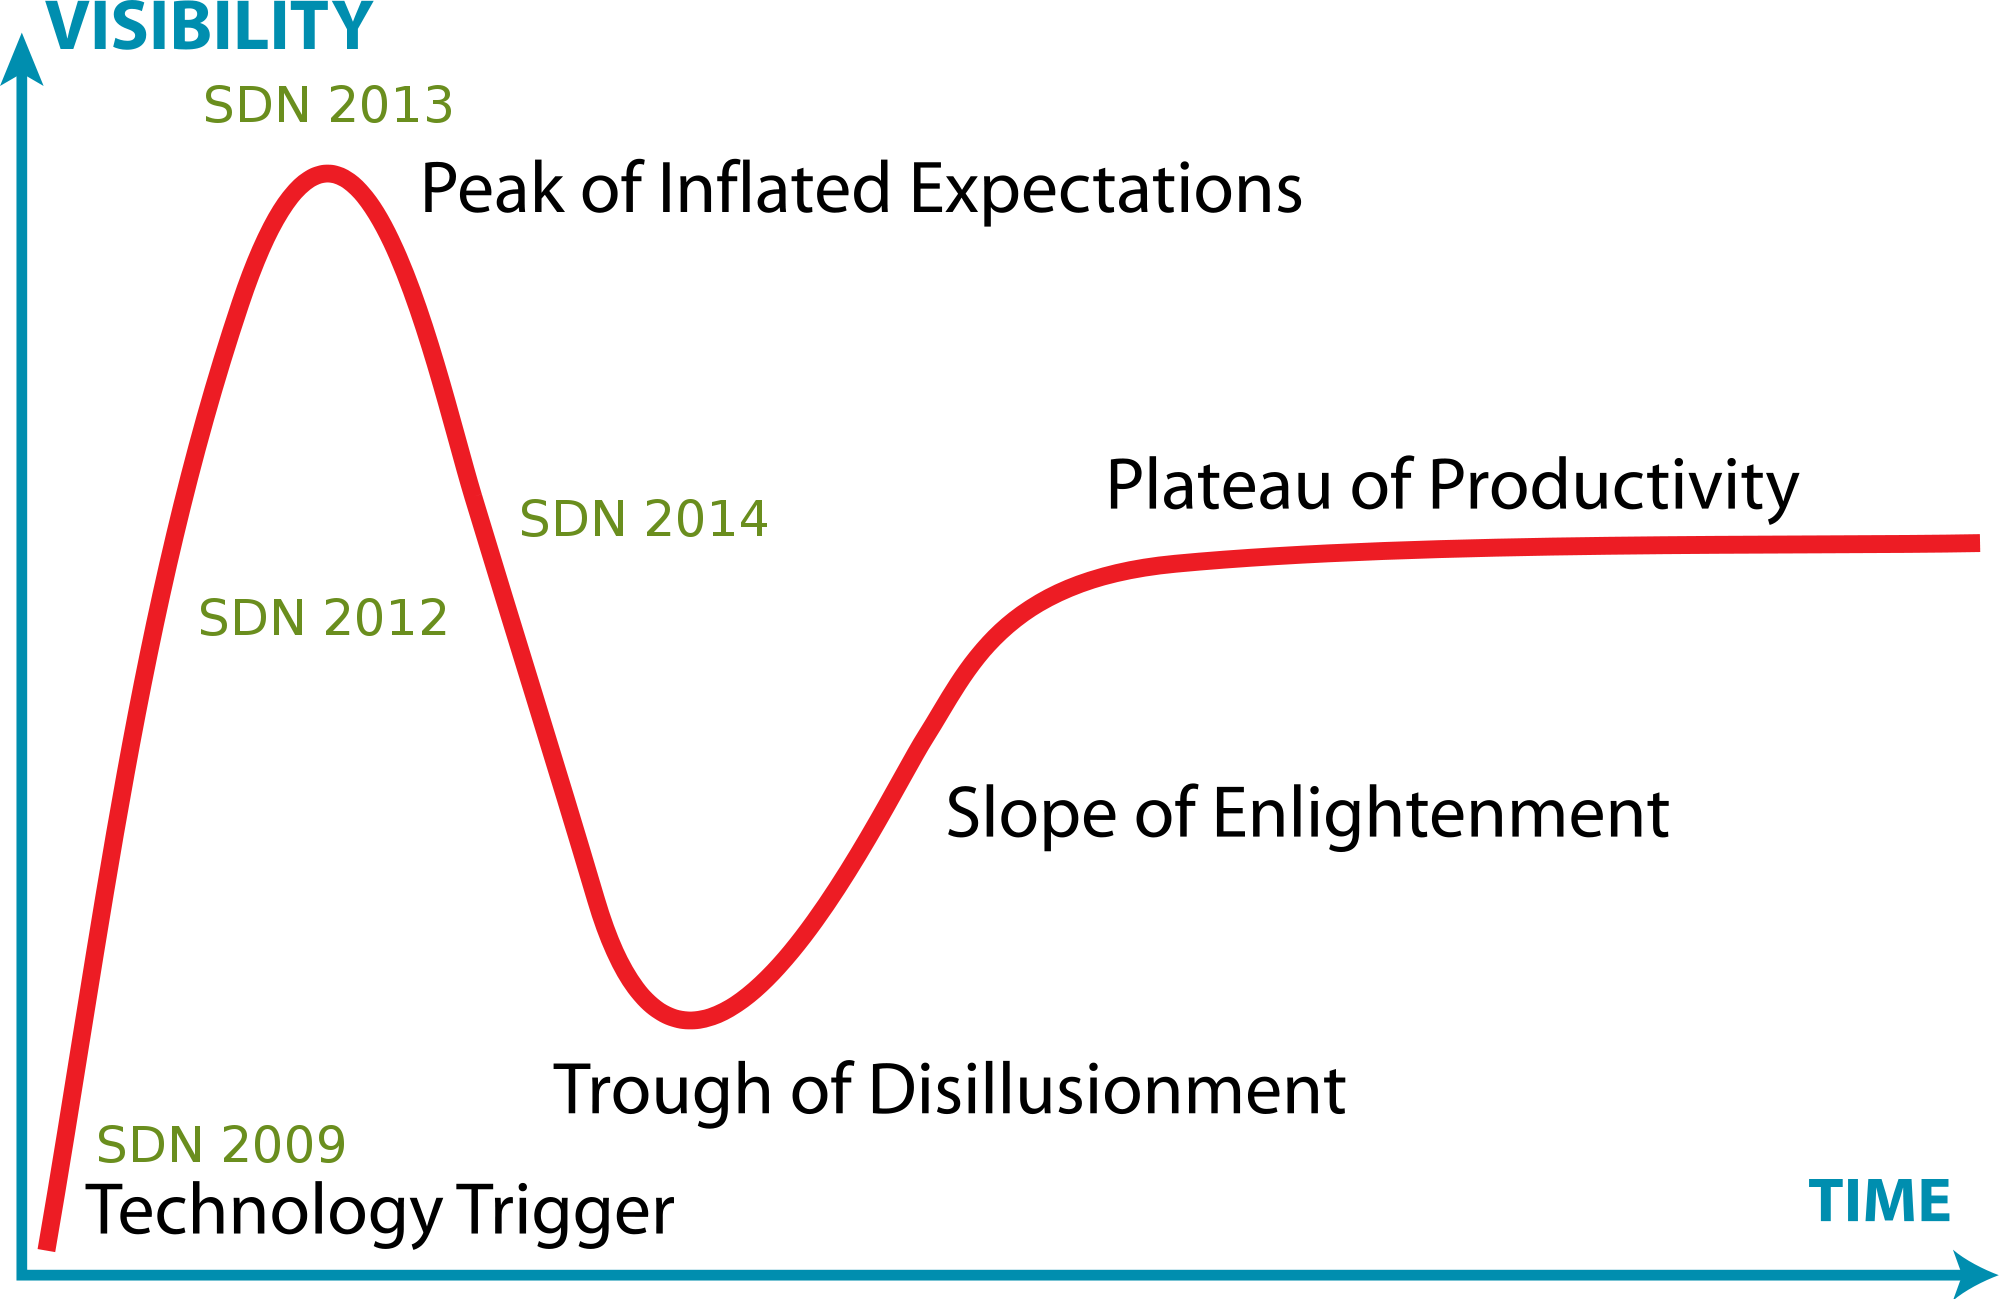
\includegraphics[width=15cm]{img/hype-cycle-03.png}
   \caption{SDN Hype Cycle}
   \label{fig:sdn_hype_cyle}
 \end{center}
 \end{figure}
\end{center}
Previous detailed issues are driving some \textbf{downward corrections on market spectations} regarding these technologies. Some reports, such as the already mentioned IDC~\cite{SDNMarket20142018IDC}, estimate that, by 2018, SDNmarket will gain ground within the broader enterprise and cloud service provider markets for datacenter networking to over \textbf{\$8B}. Other reports contemplate even worst expectations, decreasing them to \textbf{\$3.6B} by 2019~\cite{SDNMarket20142018PRNewsWire}.

\section{SDN and NFV: Business Models}
\label{sec:odlbusinessmodels}

\section{SDN and NFV with OpenDaylight: Customer Win}
\label{sec:odlbusinessmodels}

\section{OpenDaylight: Economic Aspects to go Open Source}
\label{sec:odlopensource}
Apart from the previous considerations regarding economic aspects behind SDN/NFV technologies, it is \textbf{important to analyze the economic reasons of the OpenDaylight project}.

\subsection{Technology Adoption}
The first factor to remark about SDN/NFV in general, and OpenDaylight project in particular, is \textbf{how impressive is to see major heavyweight users of networking like Ericsson, Cisco, or Juniper, together with heavyweights of IT and Operating System industries, such as HP, IBM, Microsoft, Red Hat or Citrix}.\\
\\
What are the reasons of different competitor companies to cooperate among them on an Open Source project? It is not the first time when this situation takes place. Other similar cases, such as \textbf{Webkit Open Source Project}, made competitors such as Google and Apple cooperate around development of a particular technology, in this case a Web Browser Engine.\\
\\
In the OpenDaylight Open Source project, the key words of big competitors cooperating are \textbf{``help accelerate the development of technololgy''}. In the project website~\cite{OpenDaylightAbout}, this seems to be the main reason:
\begin{verbatim}

With OpenDaylight, a community has come together to
fill this need through the combination of open community
developers and open source code and project governance
that guarantees an open, community decision making
process on business and technical issues. Establishing
an open source project in this way is designed to help
accelerate the development of technology available to
users and enable widespread adoption of SDN and create
a solid foundation for NFV.

\end{verbatim}
Neela Jacques, executive director of OpenDaylight, has pointed out in more than one occasion~\cite{NFVZoneOpenDaylight}:
\begin{verbatim}

The industry needs to create a platform that encourages
both innovation for the common good while not disturbing
the ability of members to create and sustain their own
differentiated value for their customers.

\end{verbatim}
\textbf{It is also a remarkable fact how important is, in the history of communications, the adoption of standards and terms and conditions for interoperability}. OpenDaylight is an effort of the industry to produce open source software and standards on SDN/NFV networking technologies, so that this technologies adoption is faster. From Neela Jacques perspective, \textbf{Open Source} has some disadvantages as well, but it is, no doubt, \textbf{the best way to reach interoperability}:
\begin{verbatim}

Open source maybe imperfect as a way to move forward
but it beats the tyranny of looking for an authoritarian
dictator in the market and possible interoperability issues.

\end{verbatim}
\textbf{Islands of communications were never good for anyone long-term and such will be the case with SDN and NFV}. Meanwhile, over the years, \textbf{Open Source} efforts have shown that communal efforts based on freely contributed intellectual property that is tested and honed \textbf{does not foreclose the ability to make money}.\\
\\
It historically can be argued \textbf{what it does is to expand the opportunities for success, as Open Source has long ago shed its pejorative connotations, and rightfully can be seen as being open for business}. The project should be seen as the chance for the industry to break through and score~\cite{NFVZoneOpenDaylight}, as \textbf{Open Source, due to its transparent nature, usually acts as a demonstration laboratory to show the technology, ``AS IS''}.

\subsection{The Operator's View}
In the end, there is a mandatory perspective to take into account, which is \textbf{customer opinion}. SDN/NFV technologies will be in the end new technologies to adopt, and adopters' view of drivers, barriers, timelines and targets for both technologies, as well as the role that open systems and open source play in its advancement and adoption need to be studied.\\
\\
In this sense, \textbf{OpenDaylight is well aware of the industry requirements}. To investigate issues that arouse, \textbf{SDN, NFV and Open Source Report}~\cite{SDNandNFVOperatorsView} was driven by both \textbf{OpenDaylight Open Source project together with Gigaom Research}~\cite{GigaomResearch}. This report surveyed 600 IT decision makers and technologists in medium to large organizations within enterprise (300) and service provider (300) organizations in North America~\cite{SDNandNFVOperatorsView}.\\
\\
Previously report's survey covered several main sections:
\begin{enumerate}\itemsep0pt
\item{\textbf{Demographic Questions}}. Data regarding number of employees, location servers, SDN adoption, etc.
\item{\textbf{Current State of The Network}}. Questions about cost of networking equipment and operations, end user satisfaction, business management satisfaction or open systems consideration.
\item{\textbf{SDN Benefits and Challenges}}. This section asked for ratings on SDN benefits and challenges, from lower capital expenses (CAPEX) and operating expense (OPEX), to the biggest impacts or the current SDN vendor offerigns satisfaction.
\item{\textbf{SDN/NFV and Open Source Technology}}. Obviously, \textbf{the main section to analyze from Open Source perspective}. On this part of the survey, the view of the surveyed professional related with the Open Source Technology was investigated through next questions:
\begin{itemize}\itemsep0pt
\item{\textbf{What is your view of the role of industry standards and open systems in the development and deployment of SDN/NFV solutions?}}. Available answers were from ``Critically important'' to ``Non important at all''.
\item{\textbf{What is your view of the role of open source technology in the development and deployment of SDN/NFV solutions?}}. Available answers were from ``Critically important'' to ``Non important at all''.
\item{\textbf{What are the biggest advantages of applying open source technology to SDN/NFV solutions and deployments? (Select three.)}}. Different advantages were proposed: 
\begin{enumerate}\itemsep0pt
\item{Avoiding vendor lock-in}.
\item{Lower acquisition and maintenance costs}.
\item{Gain access to large library of networking software systems}.
\item{Boost networking software capabilities}.
\item{Accelerate networking software enhancements}.
\item{Assure software systems interoperability}.
\item{Ease management of network -- and networking software}.
\item{Leverage top developer talent and software best practices}.
\item{Other (Please specify.)}
\end{enumerate}
\item{\textbf{What are the biggest drawbacks of applying open source technology to SDN/NFV solutions and deployments? (Select three.)}}. Different drawbacks were proposed: 
\begin{enumerate}\itemsep0pt
\item{Lack of commercial vendor support}.
\item{Incompatible with existing network}
\item{Performance shortcomings}
\item{Feature shortcomings}
\item{Reliability concerns}
\item{Security concerns}
\item{Deployment challenges – e.g., increased integration and test burden}
\item{Operational complexity – e.g., non-standard management interfaces and tools}
\item{Legal concerns – e.g., license management and compliance}
\item{Other (Please specify.)}
\end{enumerate}
\item{\textbf{Rate 1 to 5, your intention to apply open source technology to the following SDN/NFV functions (1 being least likely to apply and 5 being most likely to apply).}}
\begin{enumerate}\itemsep0pt
\item{SDN controller}
\item{Network automation}
\item{Network monitoring and analytics}
\item{Northbound APIs}
\item{Southbound APIs}
\item{Policy management}
\item{Security services – e.g., firewall, intrusion prevention…}
\item{Network optimization – e.g., application delivery controller, WAN optimization…}
\item{Orchestrator – e.g., OpenStack and associated plug-ins}
\item{Hypervisor – e.g., Kernel-based Virtual Machine (KVM)}
\item{Other (Please specify.)}
\end{enumerate}
\end{itemize}
\end{enumerate}
Analyzing the results of the report is critical to understand \textbf{how important is Open Source and Open Systems perceived from IT professionals}. Indeed, \textbf{the results were incredibly in favour of Open Source and Open System when talking about SDN/NFV adoption}.\\
\\
Survey results further raise the importance of open source in considering SDN and NFV solutions. \textbf{94.9\% look at open source as a positive attribute of any SDN or NFV solutions}. In particular, 9\% consider open source an absolute requirement for final selection, while 48.5\% consider it a key factor for final selection. 37.2\% believe it is a possitive attribute, although it is not a priority for the selection. Meanwhile, only 0.5\% consider open source to be a negative attribute when making final selection.
\begin{center}
 \begin{figure}[H]
 \begin{center}
   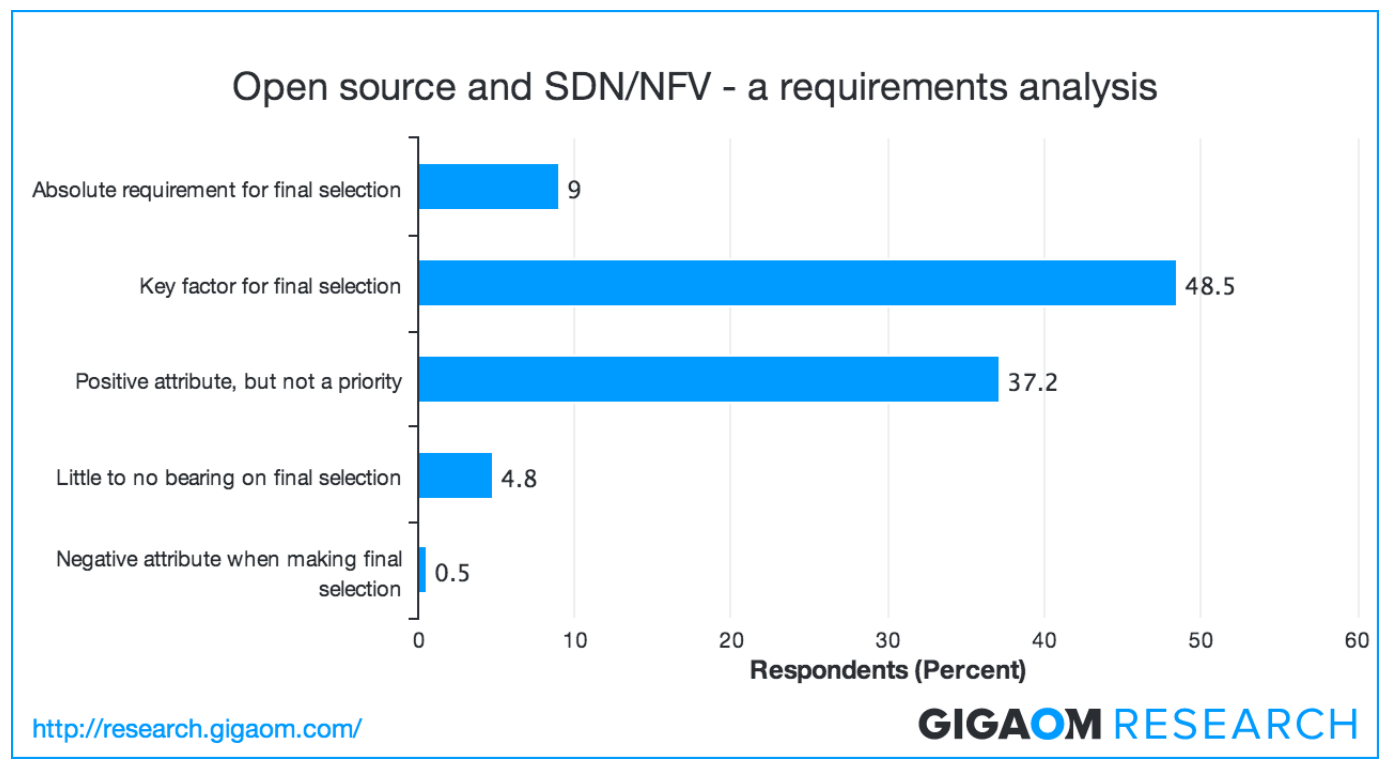
\includegraphics[width=15cm]{img/open-source-requirement-operator-view-00.png}
   \caption{Open Source on SDN/NFV - A requirement analysis}
   \label{fig:sdn_hype_cyle}
 \end{center}
 \end{figure}
\end{center}
The other important conclussion reached from the report is the \textbf{perception of the importance of open source for SDN and NFV success}:
\begin{itemize}\itemsep0pt
\item{76 percent of respondents consider open systems as critically or very important to SDN and NFV}.
\begin{itemize}\itemsep0pt
\item{18.3 percent consider it critical.}
\item{57.8 percent consider it very important.}
\end{itemize}
\item{An almost matching 68.5 percent of respondents view open source as critically or very important to SDN and NFV}.
\begin{itemize}\itemsep0pt
\item{13.5 percent consider it critical.}
\item{55 percent consider it very important.}
\end{itemize}
\end{itemize}
To summarize, the conclussion drawn is clear : \textbf{``Open Source serves as the principal delivery mechanism for SDN and NFV solutions based on industry standards and open systems''}.
\begin{center}
 \begin{figure}[H]
 \begin{center}
   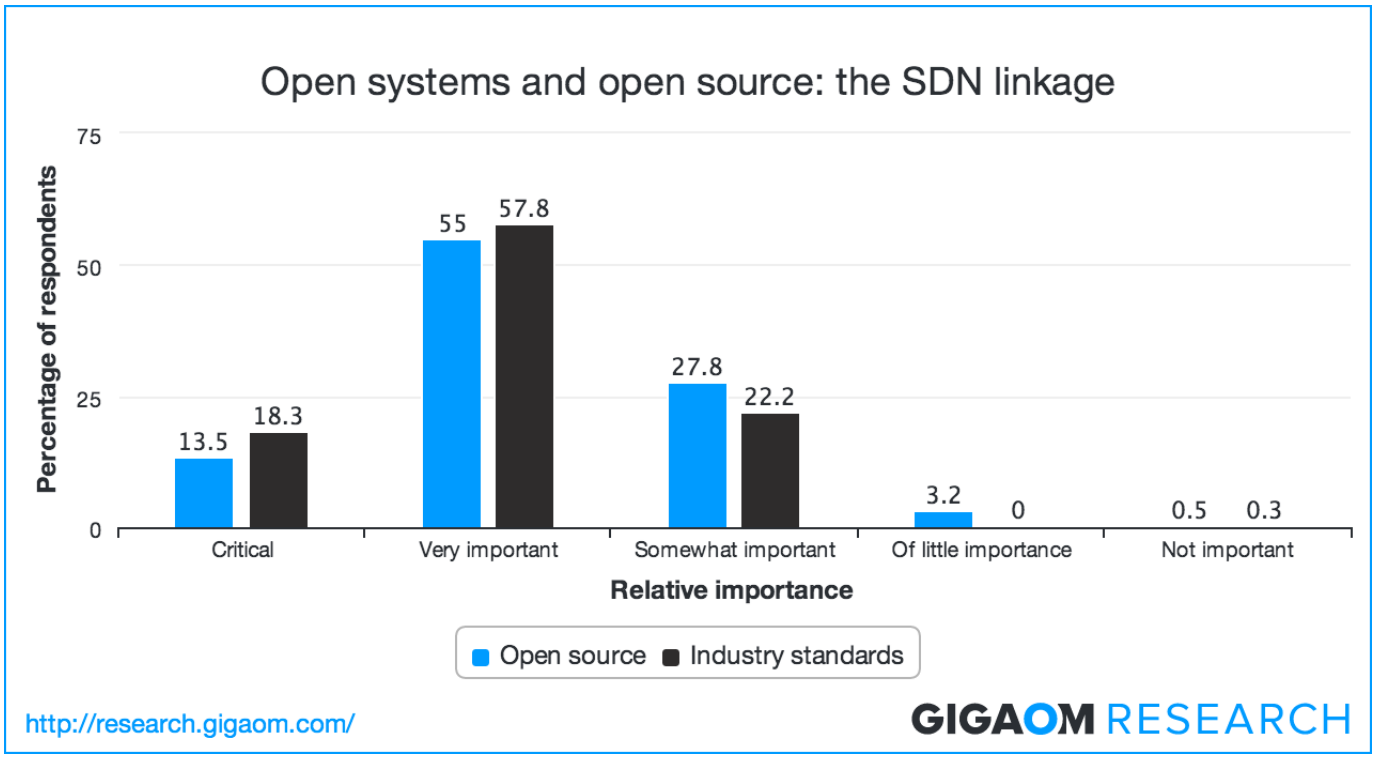
\includegraphics[width=15cm]{img/open-source-success-operator-view-00.png}
   \caption{Open Systems and Open Source: The SDN linkage}
   \label{fig:sdn_hype_cyle}
 \end{center}
 \end{figure}
\end{center}
To summarize, Open Source has indeed become mainstream, representing what IT users have come to expect from new technologies solutions over Open Source and Open System on last years: \textbf{maturity, robustness, and reliability}.\\
\\
It must be highlighted, as final conclussion, that, \textbf{from an economic perspective, going Open Source is not only desirable, but rather be mandatory to avoid future customer pejorative perception for being a closed solution}.

\chapter{OpenDaylight: Legal Aspects}
\label{chap:odllegal}

\section{OpenDaylight License: EPLv1.0}
\label{sec:odllicense}

OpenDaylight project has been released under EPL (Eclipse Public License)-v1.0~\cite{EPLv1}. This license, detailed in Appendix~\ref{chap:appendix_eplv10}, that was launched in February 2004, is considered an \textbf{Open Source Software License} due to basically two reasons:
\begin{enumerate}\itemsep0pt
 \item {It guarantees the ``Four Freedoms'' that Open Source must guarantee}:
  \begin{itemize}\itemsep0pt
   \item{Freedom to use}.
   \item{Freedom to inspect}.
   \item{Freedom to copy and redistribute copies}.
   \item{Freedom to modify and redistribute modified versions}.
  \end{itemize}
 \item {It is considered also \textbf{Open Source/Free Software} due to the fact that the two main groups having to do with this kind of softare recognizes the license to be Open Source/Free Software}:
  \begin{itemize}\itemsep0pt
   \item{\textbf{Open Source Initiative}~\cite{OpenSourceInitiative}}. This corporation recognizes EPLv1.0 not only among the ones considered to be an \textbf{Open Source license}, but also \textbf{one of the most popular ones}~\cite{OSILicenses}.
   \item{\textbf{Free Software Foundation}~\cite{FreeSoftwareFoundation}}. This nonprofit organization recognizes this license to be a \textbf{Free Software license}, although \textbf{EPLv1.0 is not compatible with GNU GPL}~\cite{FSFLicense}.
  \end{itemize}
\end{enumerate}
Taking into consideration that EPLv1.0 is Open Source, a deeper anaylisis of this license must be performed. Before analysing which kind of Open Source software license is EPLv1.0, a classification of the different kind of Open Source licenses should be performed. However, before doing such analysis, a concept related to Open Source license, which is \textbf{Copyleft}, must be introduced. According to FSF~\cite{FSFCopyleft}:
\begin{verbatim}
Copyleft is a general method for making a program
(or other work) free, and requiring all modified
and extended versions of the program to be free as well.
\end{verbatim}
However, this definition is not as concrete as it should. Although the term ``Copyleft'' was defined by FSF, OSI defines the concept in a much more understandable way~\cite{OSICopyleft}:
\begin{verbatim}
"Copyleft" refers to licenses that allow derivative works
but require them to use the same license as the original work.
For example, if you write some software and release it under
the GNU General Public License (a widely-used copyleft license),
and then someone else modifies that software and distributes
their modified version, the modified version must be licensed under
the GNU GPL too.
\end{verbatim}
Taking into consideration previous concept, according to the kind of licenses and if they are copyleft licenses or not, it is usual to follow this \textbf{classification regarding Open Source Software Licenses}:

\begin{itemize}\itemsep0pt
 \item{\textbf{Minimalistic/Academic Licenses}}: These kind of \textbf{No Copyleft} licenses are the most simple ones. \textbf{None of them has Patent Software clauses}, and they \textbf{rarely mean uncompatibilities} with other kind of licenses. This kind of license is normally very well considered (for both parts, open source and privative industry). They usually contain a \textbf{No warranty" clause}, and normally have \textbf{no restrictions}. They usually suppose \textbf{no legal complexity}. The most popular of this kind of licenses are:
   \begin{itemize}\itemsep0pt
    \item{BSD License}.
    \item{ISC License}.
    \item{MIT License}.
   \end{itemize}
 \item{\textbf{Permissive Licenses}}: This kind of \textbf{No Copyleft} licenses are similar to the academic ones, but they normally include some kind of restriction or punctualisation. This kind of restriction is normally related to \textbf{Patent Software clauses}. They \textbf{rarely mean uncompatibilities} with other kind of licenses, \textbf{although there are exceptions}. Among this kind of licenses, \textbf{the most popular one is Apache License}.
 \item{\textbf{Weak Copyleft Licenses}}: This kind of \textbf{Weak Copyleft} licenses contain copyleft clauses with certains limitations. They normally define that \textbf{not all derivative works must the copyleft license}. Derivative works inherits or not the license often depending on the manner in which it was derived. They are normally considered \textbf{Copyleft oriented to just source files}. The most popular of this kind of licenses are~\cite{FSFLicense}:
   \begin{itemize}\itemsep0pt
    \item{Mozilla Public License}.
    \item{Common Public License}.
    \item{\textbf{Eclipse Public License}}.
   \end{itemize}
 \item{\textbf{Copyleft Licenses}}: This kind of \textbf{Copyleft} licenses contain \textbf{strong clauses related to redistribution of derivative works}. This kind of licensing was first introduce by FSF, and is not well considered because of its \textbf{``viral character''}. The most popular license of this type is \textbf{GNU Generic Public License (GPL)}.
\end{itemize}
Once described the classification of Open Source licenses, it has been asserted that EPLv1.0 is classified as a \textbf{Weak Copyleft} license, as recognized by FSF~\cite{FSFEPL}. But, apart from that, inspecting the EPLv1.0 license, it can be found that \textbf{there is a possibility to distribute software under on its own license agreement}~\cite{EPLv1}, when distributing ``object code'':
\begin{verbatim}
3. REQUIREMENTS
A Contributor may choose to distribute the Program in
object code form under its own license agreement,
....
When the Program is made available in source code form:
a) it must be made available under this Agreement; and
b) a copy of this Agreement must be included with each copy
of the Program.
\end{verbatim}
As demonstrated above, there are some conditions in the license that allow this software to be distributed under other kind of license. However, if distributing source code, distribution must be performed under same agreement. \textbf{This kind of clauses are the ones that make this kind of licenses to be known ``Copyleft oriented to source files''}.\\
\\
A more detailed description of the EPLv1.0 is detailed below ~\cite{EPLv1overview}:
\subsection{History Of The Eclipse Public License}
Born in 1999, The Eclipse Public License began life within the IBM Corporation as the \textbf{IBM Public License} (IPL). IBM was willing to release open source code, but felt that needed to draft their own new licence to meet their specific needs. IPL named IBM Corporation as the licensor of code that it covered, unfortunately. That issue meant that the license could not easily be reused by others to cover code their own code.\\
\\
As a result, when IBM came to create a revised version of their licence in 2001 they generalised the terms to remove direct reference to themselves and renamed it the \textbf{Common Public License} (CPL). In 2001, IBM formed a consortium of interested technology companies around the platform including themselves, Borland, SuSE and Red Hat, and, at that same time, \textbf{IBM released their software development platform Eclipse under the CPL}.\\
\\
By 2003 it was decided that the Eclipse platform needed its own legal entity to manage code contributions coming from so many disparate sources. At the same time, the consortium had expanded to include over 50 members. Besides this, the CPL was revised in two ways to ease the establishment of the Foundation.\\
\\
On the one hand, the ‘steward’ organisation for the licence was changed from being IBM to being the Foundation itself. \textbf{This helped cohesion of the Foundation’s members} by ensuring that authority to issue revised versions of the licence in the future.\\
\\
On the other hand, it was decided that one term of the so-called \textbf{``patent-retaliation'' clause within the CPL should be revised}. The CPL states that a licensee will lose their licence to use adapt and distribute the code if they start litigation alleging infringement of a patent of theirs by the CPL-covered code. This clause was retained. However the CPL also states that if a licensee starts any software-patent-related litigation against any contributor to the code, then they also lose their licence. This would be true even if the litigation related to some entirely different piece of software..\\
\\
The \textbf{CPL has now been retired by IBM}, and \textbf{the Open Source Initiative recommend the use of the EPL in its place}.

\subsection{Main Features of EPLv1.0}
The \textbf{EPL grants the ``Four Freedom'' rights}, as shown before. However, the license enumerates the rights granted as follows:
\begin{itemize}\itemsep0pt
 \item{Licensee has the right to copy, adapt and distribute the program in source or object code form}.
 \item{Licensee has the right to distribute the code in object code form alone under a different licence, provided that licence is compatible with the EPL}.
 \item{Licensee has the patent rights from all contributors to use and make available the code}.
  \item{Licensee has the right to distribute works which contain the code in combination with new code modules, and to license the new code modules in any way the distributor wishes}.
\end{itemize}

To summarise the most important parts of the EPL, it must be highlighted that EPL:
\begin{itemize}\itemsep0pt
 \item{\textbf{Explicitly grants patent rights} where necessary to operate the software}.
 \item{\textbf{Keeps the covered code itself open source}}, due to its ``Weak Copyleft'' nature.
 \item{\textbf{Allows expansion of the code via new modules that can be licensed in non-open ways}}.
\end{itemize}\itemsep0pt

\subsection{Other Software Development Considerations}
Some considerations must be taken into account regarding the consideration that the Eclipse Foundation provides about the EPLv1.0 license:
\begin{enumerate}
 \item{The Eclipse Foundation makes clear that, in their opinion, ``merely interfacing or interoperating'' with an Eclipse plugin does not make your code a derivative work of the plugin}.
 \item{Therefore original software developed using the Eclipse platform can bear any licence its author chooses when distributed}.
\end{enumerate}

Once EPLv1.0 license has been analyzed and classified, it must be analyzed \textbf{which reasons make OpenDaylight Open Source project} to use this kind of license. In the FAQ section of OpenDaylight Open Source project, next statement appears~\cite{OpenDaylightFAQ5}:

\begin{verbatim}
5. What license will the project use? Why was that decision made?

OpenDaylight is structured and governed using open source best
practices and is licensed under the Eclipse Public License-v1.0
(EPL), which is a common choice for Java-based projects. The EPL
is an approved open source license by the Open Source Initiative
and considered a free software license by the Free Software
Foundation. The license choice of EPL maximizes OpenDaylight’s
license compatibility with the large ecosystem of libraries and
3rd party components that have already been released under the EPL
license. Where necessary the Board may approve exceptions for other
licenses.
\end{verbatim}
Basically, the reasons for using this kind of license are basically three:
\begin{itemize}
 \item{\textbf{Open Source/Free Software license}}. Being recognized by both OSI and FSF, this license is suitable into the structured and governance bylaws of the project having to do with its Open nature and commitment to the Open Source movement.
 \item{\textbf{Java-based project}}. EPLv1.0 is a common license for Java-based projects. Being \textbf{developed in Java programming language primarily}, OpenDaylight Open Source project fits quite well into this kind of license, as other projects written in Java do, as, for instance, Eclipse IDE.
 \item{\textbf{3rd party libraries/components compatibility}}. Last, but not least, Board in OpenDaylight decided that \textbf{EPLv1.0 license fits better in terms of compatibility with 3rd party components and libraries used} inside the project compared to other kind of licenses. Examples of 3rd parties used in OpenDaylight Open Source project are Java programming language, Maven, Open vSwitch or Open Flow Java implementation.
 \item{\textbf{Avoid licensing fragmenation}}. Using this kind of ``Weak Copyleft'' license helps on avoiding licensing fragmentation for derivative works/forks/spinoffs. A more detailed information on how fragmentation is avoided appears on Section~\ref{sec:otherlicensebylaws}.
\end{itemize}
Up to this point, EPLv1.0 and OpenDaylight Open Source project to use this license have been analysed. In next section, other legal considerations and Bylaws will be studied in order to clarify other important issues that are considered inside OpenDaylight Open Source project to be important as well.

\section{Other Licensing Considerations}
\label{sec:otherlicenseconsiderations}

On previous section EPLv1.0 license and its application to the OpenDaylight Open Source pr oject were studied. However, there are \textbf{other licensing considerations} to take into account by the project and its Governance Board.\\
\\
For this reason, having a look at the FAQ of OpenDaylight Open Source Project~\cite{OpenDaylightFAQ}, other legal considerations must be taken into account:

\begin{verbatim}
8. Will all development be done in the open?
All OpenDaylight source code development will be done
in the open. Some contributors or companies may choose
to incubate and develop code internally and then contribute
it openly later, which is fine as well, but the core project
code will all be developed in the open for everyone to see
and use under a standard OSI-approved EPL open source license.
\end{verbatim}
Previous statement tries to perform as a \textbf{declaration of intent} by the project Governance. In particular, it tries to clarify the intention of perform development of the core project with an Open Source licensing scheme, \textbf{clarifying the intention to use EPL Open Source license} as a general rule to guarantee open development.

\begin{verbatim}
17. Will the products developed on the framework also be
open source?
This is the sole discretion of each company. The intent of
OpenDaylight is to employ collaborative, open source development
to build and support an open source framework and codebase on top
of which commercial products and services can be built. How each
vendor adopts OpenDaylight and commercializes their own products
will be an individual business decision for them, subject to the
Eclipse Public License.
\end{verbatim}
With previous statement, the OpenDaylight Open Source Project Governance tries to clarify the discretion of each company to perform \textbf{whichever commercial actions they consider}, taking into account the Eclipse Public License and the different statements appearing on it. Far from being commercially agnostic, this statement is a nod to empower companies to use this Open Source project as a base to commercialize products and services.

\begin{verbatim}
19. How will OpenDaylight prevent fragmentation?

Many open source projects eventually see forks or spinoffs
from the original codebase. Experimentation and innovation
off of an open source codebase is common and encouraged.
However, long term the open governance and open technical
decision making structure employed by the OpenDaylight
project should help minimize the need to do any significant
fragmentation from the core project codebase.
Further, OpenDaylight employs an OSI approved open source
license. The EPL requires any distributed modifications to
the program also be licensed under the EPL. For more
information on the EPL, see the Eclipse EPL FAQ.
\end{verbatim}
\noindent Previous statement is a clarification about the \textbf{decission to use EPL} to minimize forks of the original codebase. This license usage does not guarantee forks/spinoffs of the project are not taking place, but, at least, guarantees them to be Open Source if the source code is modified and wants to be distributed. In next section, \textbf{Bylaws of OpenDaylight Open Source project} will be summarized. Far from being analysed in a deep basis, the most important statements in the project bylaws are to be enumerated in order to \textbf{clarify those legal statements} that must be taken into consideration.

\section{Bylaws}
\label{sec:bylaws}
Adopted by July 28, 2014, OpenDaylight Project Inc. contains a set of thirteen articles to clear up all the different issues from a Legal and/or Governance perspective. The document, known as ``Second Amended And Restated By-Laws''~\cite{OpenDaylightBylaws}, is summarized in Appendix~\ref{chap:appendix_bylaws}, and define a complete legal statement that considers several aspects having to do with:
\begin{enumerate}\itemsep0pt
 \item{\textbf{Name, Purpose and Offices}}. This Article focuses on some legal aspects such as the name of the company, the offices or the purpose and non-profit status of the project.
 \item{\textbf{Members}}.  This Article summarizes the different kind of members and the conditions of membership of the OpenDaylight project.
 \item{\textbf{Actions of Members}}. Different kind of actions that members can carry out are collected on this Article.
 \item{\textbf{Directors}}. This Article focuses on the different responsabilities and rights that directors own.
 \item{\textbf{Executive Committee and Other Committees}}. On this Article a clarification of how an Executive Committee can be created or modified, as well as how other Committess can be composed in order to perform general or special duties or how meetings of the Executive Committee will take place.
 \item{\textbf{Officers}}. A complete description of the Officers, their role in OpenDaylight Open Source project, vacancies, their election, tenure, executive role, vice-president roles, secretary role, treasurer role and compensation fees is provided in this Article.
 \item{\textbf{Notices}}. Information regarding notifications, communication and electronic transmission to any Director or Member of OpenDaylight Open Source project.
 \item{\textbf{Indemnification}}. Actions regarding the Rights of the ODP, Success on the merits, Authorization, Advance Payments, Non-Exclusivity clauses, Jurisdiction, Insurance or Severability are some of the aspects covered in this Article.
 \item{\textbf{Books And Records}}. Stuff related to Books and Records of Account are handled on this Article.
 \item{\textbf{Certain Transactions}}. A complete analysis of the conditions of the transactions with interested parties and OpenDayligth members (Directors, Officers, etc.) are cleared up on this article.
 \item{\textbf{Grants, Contracts and Loans}}. Information about grants and contribution authorization, contract execution, and finance products such as checks, drafts or deposits are handled in this Article.
 \item{\textbf{General Provisions}}. Fiscal Year, Reserves, corporate Seal adoption or Proprietary Rights are discussed on this Article.
 \item{\textbf{Antitrust Compliance}}. A complete and detailed Article about antitrust and competition laws, Availability of Intellectual Property and Obligations to Endorse.
 \item{\textbf{Amendments}}. Conditions of alterations and amendments to bylaws.
\end{enumerate}

\chapter{OpenDaylight: Governance and Community Management}
\label{chap:odlcommunity}

This chapter summarizes the state of the OpenDaylight project from management perspective. Different important aspects for an open source project, related to the community that makes it up and its governance will be analyzed, such as:
\begin{itemize}\itemsep0pt
\item{\textbf{Project Governance}}. Aspects such as decission taking, how board of directors is established and different aspects having to do with the way the project is governed are handled on this subchapter.
\item{\textbf{Community Management}}. An enumeration of the different tools available for the community to contribute to the project will be analyzed. Besides this, communication channels and strategy, marketing campaigns of the project, community project rules, organization politics, entry barriers and other similar points in OpenDaylight project are studied in this chapter.
\end{itemize}

\section{OpenDaylight Project Governance}
\label{sec:odlgovernance}

OpenDaylight project intention from a governance perspective is to ease an open ecosystem, not only from the software perspective, as it is provided with an open source license, but also from other areas that are as important as software development. OpenDaylight is structured to be \textbf{Open}:
\begin{itemize}\itemsep0pt
\item{\textbf{Open Design}}.
\item{\textbf{Open Development}}.
\item{\textbf{Open Contribution}}.
\item{\textbf{Open Governance Model}}.
\end{itemize}
Being a Linux Foundation Collaborative Project, OpenDaylight implements many open source best practices that are familiar to other leading projects of that same organization. Besides ths, any individual, company or organization can engage directly and immediately to begin shaping the future of the project, as OpenDaylight is \textbf{open to anyone}.\\
\\
Anyone can develop and collaborate, whether code, documentation or any other kind of contribution. Anybody can also be elected to be part of the governance of the project, turning into a project leader and providing leadership regarding the technical direction of OpenDaylight. There are basically two groups that compose the goverance of the OpenDaylight project:

\subsection{Technical Steering Committee (TSC)}
Among the responsibilities of the TSC, tasks as technical best practices (including the Development Process), simultaneous release dates, quality standards maintainence, technical progress monitoring, technical conflicts mediation and resolution between committers and project leads or inter-project collaboration organization. The TSC oversees the design and development activities carried out in the OpenDaylight project, as outlined in the \textbf{TSC Charter~\cite{OpenDaylightTSCCharter}}. This document, appearing on Appendix~\ref{chap:appendix_tsccharter}, contains a collection of sections defining the different considerations that must rule the OpenDaylight project from a technical view:
\begin{itemize}\itemsep0pt
\item{\textbf{Section 1. Guiding Principle}}. Defines the project operation principles. It defines that project proposals, timelines and status \textbf{must not merely be open, but also easily visible to outsiders}. To do so, the project \textbf{will operate transparently, openly, collaboratively, and ethically}.
\item{\textbf{Section 2. Evolution of ODP Governance}}. This section defines the existence of two areas of governance. \textbf{TSC performs Technical leadership}, while \textbf{Board of Directors} is responsible of \textbf{business leadership}.
\item{\textbf{Section 3. Board's role}}. Clarification on the Board's role is described in this section. Typically, \textbf{the board have no say in technical issues}, although it sets overall project policy and scope.
\item{\textbf{Section 4. TSC Establishment}}. Mechanisms to elect TSC members are summarized on this section. Initially, \textbf{TSC shall be formed by representatives designated by Platinum members}. However, active Committers will elect in the future a number of TSC members, still to be determined. Platinum members may designate a TSC, although this is expected to be a temporary measure.
\item{\textbf{Section 5. Resposibilities of the TSC}}. Definition of the different task where TSC is responsible appear on this section of the Charter. \textbf{Technical best practices, release dates and quality or technical conflict mediation are the main responsibilities} of this committee.
\item{\textbf{Section 6. Operations}}. Description of the \textbf{Development Process} is described on this section. Life-cycle process, Core projects and changes approval criteria (cleanliness of code base, statibility, predictability, etc.), are defined.
\item{\textbf{Section 7. Project Roles}}. Definition of the roles to consider on the project are defined under this section. Basically, three kind of roles are defined:
\begin{enumerate}\itemsep0pt
\item{Committers}. People who has rigth to commit to one or several projects. Rights and obligations are defined.
\item{Project Leads}. Project Lead, which is \textbf{unique per project}, are Commiters selected by vote, unless only one committer exist.
\item{Contributors}. People contributing to the project but without commit permission.
\end{enumerate}
\end{itemize}
This commitee is also responsible of defining the guidelines of the \textbf{TSC Policy~\cite{OpenDaylightTSCPolicy}}. This document, which appears on Appendix~\ref{chap:appendix_tscpolicy}, has been \textbf{set by the Board of Directors}, defines policies to govern the operation of the TSC, \textbf{related to release process, technical scope, business goals, etc)}. TSC must adhere to these policies to the best of its abilities.\\
\\
In the end, these policies are a set of \textbf{guidelines that apply to the projects existing under OpenDaylight, the artifacts created, its operation and scope}. TSC Policies emphasize aspects that must cover previous statements, such as:
\begin{itemize}\itemsep0pt
\item{\textbf{Singularity}}. To avoid overlapping goals between projects.
\item{\textbf{Cohesiveness}}. To form a cohesive system where all projects connect between them.
\item{\textbf{Simultaneous Release}}. To ensure release at regular intervals in a ``release often, release early'' basis.
\item{\textbf{Communication}}.  To emphasize on open, fair and consistent communication within the project.
\item{\textbf{Openness}}. To ensure Technical decisions are made in an open fashion.
\end{itemize}
\subsection{Board of Directors}
As described before in TSC Charter, \textbf{Board of Directos is responsible of business leadership}. This group will not participate on technical issues or individual project scope, as long as each project remain within the direction of the policies defined by the Board of Directors. Board of directors will be rather responsible of:
\begin{itemize}\itemsep0pt
\item{\textbf{Set overall project policy}}. In consultation with TSC, policies will be decided.
\item{\textbf{Describe aggregate scope of projects}}. Always, without interfere on each particular project scopre.
\item{\textbf{Drive a technical vision and direction}}. By setting the tendencies and technologies driving the market and SDN/NFV state of art.
\item{\textbf{Define a release guidance to the TSC}}. In order to provide guidelines and approximate dates of releases.
\end{itemize}
The Board of Directors is composed of a group of highly qualified members, with extensive knowledge on Cloud, Virtualization, Routing, Internet Technologies and Networking in general, SDN and NFV in particular, of the most important member companies involved in the project.
\begin{itemize}\itemsep0pt
\item{\underline{\textbf{Neela Jacques (OpenDaylight Executive Director)}}}. He works with the community to adavance SDN and NFV. Formerly at VMware, developed and took to market the company’s software-defined data center vision and strategy including VMware’s vCloud Suite.
\item{\underline{Abhishek Chauhan}}. CTO and vice-president for the Cloud Networking Group at Citrix.
\item{\underline{Chris Wright}}. Technical Director of SDN at Red Hat.
\item{\underline{David Meyer}}. CTO and Chief Scientist at Brocade Communications.
\item{\underline{David Ward}}. CTO and Chief Architect of Engineering at Cisco Systems.
\item{\underline{Francois LeMarchand}}. Head of Ericsson SDN product \& solutions group.
\item{\underline{Inder Gopal}}. Responsible for all hardware and software networking products in IBM.
\item{\underline{Jennifer Lin}}. Jennifer was a member of the founding team and VP, Marketing at Contrail Systems, where she led the product management and marketing activities, until Juniper acquisition of the company.
\item{\underline{Marc Cohn}}. Senior DirectorCiena Corporation, has been a major contributor to Ciena’s Software Defined Networking (SDN) initiative, and chairs the Committee (MEC) for the Open Networking Foundation (ONF).
\item{\underline{Rajeev Nagar}}. Oversees the Core Networking team, responsible for infrastructural networking/connectivity technologies for Microsoft.
\item{\underline{Sarwar Raza}}. Director of Cloud Networking and Software Defined Networking (SDN) in the Advanced Technology Group at HP Networking.
\item{\underline{Terry Nakajima}}. Senior Manager in NEC Corporation of America, leading business strategy and engineering for NEC’s Software defined networking products.
\end{itemize}

\section{OpenDaylight Community Management}
\label{chap:odlcommunitymgmt}
This chapter will analyze aspects having to do with community management. Different tools and communication channels that the project provides to its community in order to facilitate community involvement in the project will be studied.\\
\\
Besides this, Marketing strategies will be analyzed, as well as community building and new volunteers attraction strategies. Entry barriers will be analyzed as well, by studying the different mentorship and internship programs or the available documentation for new members.

\subsection{Communication Channels}
Apart from tools related to software development and other technical stuff, OpenDaylight project provides a set of tools for community members to keep in touch and communicate each other. Apart of the aforementioned tools, there is a set of channels to help community communication:
\begin{itemize}\itemsep0pt
\item{\textbf{\underline{Social Media}}}. Far from criticism, and with emphasis on its pragmatic view, the Opendaylight project is conscious of the \textbf{importance of the Social Media}. For this reason, main Social Networks accounts have been created for communication with the community:
\begin{itemize}\itemsep0pt
\item{\textbf{Twitter}}. OpenDaylight Twitter account~\cite{OpenDaylightTwitter}, with nearly 5300 followers, important information and events are published through this tool.
\item{\textbf{Facebook}}. Not as important compared to Twitter, OpenDaylight Project Facebook page~\cite{OpenDaylightFacebook}, with 1360 Likes, is another channel where links to interviews and important events are published.
\item{\textbf{Google+}}. OpenDaylight Google+ profile~\cite{OpenDaylightGooglePlus}, with nearly 700 Google+ users on its circles, provide similar information about the community of OpenDaylight project, such as events holding, community involvement presentations or technical overview videos.
\item{\textbf{LinkdedIn}}. OpenDaylight LinkedIn profile~\cite{OpenDaylightLinkedIn}, with more than 360 followers, is a tool to communicate with this Social Network oriented to job environment. New software releases, man events to occur, new members in the project or presentation of members of the community are examples of the kind of information which is broadcasted in LinkedIn's OpenDayligt Project page.
\item{\textbf{Youtube}}. OpenDaylight's Youtube channel~\cite{OpenDaylightYoutube} has more than 800 subscribers, and owns more than 60 videos, from the introduction of the project to different HackFest speaks, tutorials and roundtables.
\end{itemize}
\item{\textbf{\underline{IRC Channel}}}. Hosted on freenode.net, the \#OpenDaylight channel hosts around some dozens of members willing to help and connect with other members of the OpenDaylight developer community.
\item{\textbf{\underline{Mail Lists}}}. Apart from previous channels, more than 100 mail lists exist to assist on different question and issues regarding a particular aspect of a particular project. There is normally one mail list per aspect of the project considered to be under discussion. For instance, ``OpenDove'' project hosts next mail lists:
\begin{table}[H]
\footnotesize
\begin{center}
\begin{tabular}{|l|l|l|}
\hline
\textbf{Mail List} & \textbf{Discussion} \\ \hline
opendove-announce	& Open DOVE Announcements (low volume) \\ \hline
opendove-bugs	& Notifications from Bugzilla for Open DOVE \\ \hline
opendove-dev	& Developer discussions for Open DOVE \\ \hline
opendove-gerrit	& Gerrit automated notices about Open DOVE \\ \hline
opendove-jenkins	& Jenkins CI notifications for Open DOVE \\ \hline
opendove-users	& Community driven support alias for Open DOVE \\ \hline
\end{tabular}
\end{center}
\caption{Example of OpenDaylight's OpenDove Project mail lists}
\label{tab:projectmaillist}
\end{table}
NOTE:PENDING:Include a list of all the available project maillists?
\item{\textbf{\underline{Blogs}}}. Blogs in OpenDaylight are a powerful and extensively used tool to communicate latest updates in the project. Two blogs stand out among the rest:
\begin{enumerate}
\item{Neela Jacques' blog}. Neela Jacques, executive director of OpenDaylight, shares his view on the different threats and oportunities around OpenDaylight project, with high focus on the Open nature of the project and technologies involved.
\item{OpenDaylight's blog}. This generic blog is more focused on broadcasting general information related to the project, from event celebration, to community member's spotlights, it also covers important update information, such as the announcement of the OpenDaylight Ambassador program, or the different new tutorials available.
\end{enumerate}
\item{\textbf{\underline{Contact Information}}}. Apart from the previous communication channels, OpenDaylight project provide a Contact Information section with the most important contact mail addresses, such as the ones for Press and Analyst Inquiries, Eveint Inquiries, Website Questions or other Information Inquiries. It also provide a form to address general inquiries.
\end{itemize}

\subsection{Community Tools}
As defined previously, OpenDaylight project is defined to be \textbf{open}, highlighting the project wish for \textbf{everybody to participate}. Every opensource project that emphasizes on community needes to provide an \textbf{infrastructure that ease all different kind of activities involved on collaboration}, not just software development, but also other very important activities such as documentation, Quality Assurance (QA), etc.\\
\\
In this sense, OpenDaylight project is not an exception, and provides several tools~\cite{OpenDaylightTools}, available to help OpenDaylight contributors and collaborators on the different tasks they want to carry out. Among the different utilities, next ones must be remarked:
\begin{itemize}\itemsep0pt
\item{\textbf{\underline{Wiki}}}~\cite{OpenDaylightWiki}. For an open source project, \textbf{it is very important to own a well structured and simple Wiki}. A project wiki is, normally, together with the FAQs, the entry point for starting contributions and potential community members. In OpenDaylight Wiki, a simple main page appears, with several important aspects such as:
\begin{enumerate}\itemsep0pt
\item{\textbf{Welcome message}}. An introductory welcome message with sign up information needed for contribution.
\item{\textbf{OpenDaylight Projects}}. With different important introductory documentation, such as \textbf{Getting Started for Developers}~\cite{OpenDaylightDevStGuide} guide, the \textbf{Getting Started for Projects}~\cite{OpenDaylightProjStGuide} guide, or the \textbf{Code of conduct}. This section includes as well infrastructure guides, Core Architectural Principles and a link to the different sub-projects existing under OpenDaylight project.  Another important reference linked from this section is the \textbf{Bugs Wiki page}~\cite{OpenDaylightBugsWiki}, with information to help on bug resolution, fields used on but reporting, etc.
\item{\textbf{Technical Collaborations}}. This section of the Wiki covers different technical collaboration spects having to do with Developer Events, Work Streams, Meetings and Committees, Intern Project Ideas and Cross Project Collaborative Groups. Other aspects, such as Simultaneous Release information for each of the upcoming releases, are also handled in this section of the Wiki.
\item{\textbf{Community}}. Last, but not least, some information regarding the Community, such as the Ambassador Program or the different presentations~\cite{OpenDaylightPresentations} of the OpenDaylight project available.
\end{enumerate}
\item{\textbf{\underline{Ask}}}~\cite{OpenDaylightAsk}. This \textbf{AskBot~\cite{AskBot} based Q\&A Forum} provides a mechanism for the community to ask their questions for other members of the community to provide help on that particular aspect. Questions appearing on this tool are usually of an \textbf{advanced technical level}, i.e.: ``how we could use an ADSAL plugin service inside of an MDSAL plugin ?''. This tool provide a \textbf{Tagging Mechanism}, where questions are classified normally by its technical area. Tags such as \textbf{REST}, \textbf{openflow}, \textbf{vlan} or \textbf{GUI} or \textbf{neutron} are examples of the tags under which the different questions on Ask are classified.
\item{\textbf{\underline{Identity}}}~\cite{OpenDaylightIdentity}. Identity utility is just a \textbf{WSO2 Identity Server~\cite{WSO2IdentityServer} based tool} to create and manage an OpenDaylight user accounts. Contributors to the OpenDaylight tools must have signed-up in Identity to publish code, review code, publish Wiki pages or perform any other contribution task. Apart from being a user account management tool, \textbf{Identity also manages different applications a particular contributor has access too}.
\item{\textbf{\underline{Bugzilla}}}~\cite{OpenDaylightBugzilla}. A \textbf{Bugzilla~\cite{Bugzilla} based Bug Tracking} web tool. In this sense, OpenDaylight project just takes advantage of this \textbf{widely used} Bug Tracking system. OpenDaylight Bugs are classified by Product (ovsdbd, for instance) and Component inside the product (API, for instance). Nearly 500 Bugs are, up to date, registered on OpenDaylight Bugzilla.
\item{\textbf{\underline{Gerrit}}}~\cite{OpenDaylightGerrit}. A \textbf{Gerrit~\cite{Gerrit} based Reviewing Code} web tool. In this sense, OpenDaylight project just takes advantage of this \textbf{widely used} reviewing code system, that easily integrates with other tools such as Jenkins and Git Source Control system.
\item{\textbf{\underline{Jenkins}}}~\cite{OpenDaylightJenkins}. A \textbf{Jenkins~\cite{Jenkins} Continuous intergration} web tool. In this sense, OpenDaylight project just takes advantage of this \textbf{widely used} continous integration system, that easily integrates with other tools such as Gerrit and Git Source Control system, to perform automatic Quality Assurance in Continouous Integration.
\item{\textbf{\underline{Nexus}}}~\cite{OpenDaylightNexus}. A \textbf{Nexus~\cite{SonatypeNexus} Repository Manager} web tool. This tool allows proxying remote repositories as well as sharing software artifacts, organize artifacts, improve collaboration across teams and source the highest quality components for use in their applications.
\item{\textbf{\underline{Sonar}}}~\cite{OpenDaylightSonar}. A \textbf{SonarQube~\cite{SonarQube} technical debt} web tool. With a very efficient way of navigating, this tool provides a balance between high-level view, dashboard, TimeMachine and defect hunting tools. OpenDaylight tracks in this tool some of the different projects, such as yangtools, OpenFlow or osvdb, to quickly uncover components that are in Technical Debt and establish action plans to fix them.
\end{itemize}

\subsection{Marketing and Community Building}
OpenDaylight project is, no doubt, following an open source strategy more alligned to the pragmatic view of open source. With high commercial view, caused mainly by the amount of big and important companies involved, and a well driven marketing strategy, this open source community is more focused on the openness aspect of the project, rather than on the idea of the Open Source Software aspect.\\
\\
Taking previous statement into consideration, it must be remarked that OpenDaylight project \textbf{has invested a big effort on project broadcasting and community involvement}. In this section, the most important aspects having to do with this aspects are analyzed. Questions such as ``How can a contributor participate in the project?'' or ``Which are the main community driven events?'' are answered in this section.\\
\\
To start with, OpenDaylight project provides some guidelines on \textbf{How to participate}~\cite{OpenDaylightHowToParticipate}. From the project's perspective, the best entry point to the project is the ``Getting Started Guide''. Apart from that, there is also an ``Events'' entry, where the most important meetings are notified. Both aspects are analyzed in this section.\\
\\
Having to do also with Marketing and Community building, some other sections from the OpenDaylight project web page, such as ``News'' or ``Resources'', are part of the marketing strategy of the project. To end this section, other groups and resources that OpenDaylight provides to achieve Community Building will be mentioned.

\begin{enumerate}
\item{\textbf{Getting Started Guide}}. This introductory guide~\cite{OpenDaylightStGuide} plays the role of starting point for any contributor, collaborator or company which is willing to participate in the community. This guide provides different starting information classified by the different kind of community roles considered, i.e.:
\begin{itemize}\itemsep0pt
\item{\textbf{For Users}}. Download software releases information and software editions are provided for the user to start playing with OpenDaylight project software. Apart from that, reference to previously described mail lists is suggested for further investigation.
\item{\textbf{For Developers}}. A list of the tools and resources available for developers to start contributing are also described. Examples of pointed resources, the previously described tools (remarking Wiki as the most important), as well as communication channels such as mail lists.
\item{\textbf{For Membership}}. Not only personal contribution, but also companies and organizations, are welcome  to join at any time and to start participating, as OpenDaylight is an open source software project. Companies and organizations interested in formal membership in the project can contact submit a request for information on the membership page~\cite{OpenDaylightJoin}.
\end{itemize}
\item{\textbf{Main Events}}. The most important marketing tool available for OpenSource project are Events. This kind of meetups are very important for people involved in the community, members, companies and in general any person, organization or community involved int the project to know each other.\\
\\
Main event regarding OpenDaylight open source project is \textbf{OpenDaylight Summit}. This \textbf{annual} event will hold its second edition in 2015 in Santa Clara, where the first edition, in 2014, was also held. First edition was a great success, with \textbf{over 600 attendees and almost 50 speakers}~\cite{OpenDaylight2014Summit}. OpenDaylight events are directly driven by the Linux Foundation.\\
\\
OpenDaylight Summit first edition was a two day event, with more than 40 speaks, covering different aspects about the OpenDaylight project in particular, but also, from a more general pespective, about all the different technical aspects, technologies and protocols involved in OpenDaylight, such as SDN, NVF, OpenFlow, Open vSwitch, Policy and Orchestration, etc, where a complete set of videos and presentations result from.\\
\\
Apart from main event, there is a set of \textbf{secondary events} organized by OpenDaylight project. Among the most important, next ones are found:
\begin{itemize}\itemsep0pt
\item{\textbf{HackFests}}. This kind of events focus on \textbf{introducing new community members}, providing hands on workshops aimed at building, through OpenDaylight platform, SDN applications. Other aspects, such as \textbf{bugfix coaching sessions}, also take place into this kind of event, to help people willing to contribute and ease the entry barriers to start. Düsseldorf or Tokyo are among the cities that have hosted this kind of OpenDaylight events.
\item{\textbf{Developer Design Forums}}. This kind of event, \textbf{focused on the developer community}, try to engage in a range of hot topics geared towards \textbf{networking}. Additionally, this kind of forum help to \textbf{set the stage for future OpenDaylight releases}.
\item{\textbf{Other events}}. Not directly associated or organized by the OpenDaylight project, the community can also receive speaks on this project as part of other events. Examples of events where OpenDaylight appeared are the \textbf{OpenStack Summit}, that will be hosted in Paris in November 2014, or the \textbf{Broadband World Forum}, that will be hosted in October 2014. Being part of such important events gives a very wide idea of the importance of the OpenDaylight project and how crucial is the role that this project can play looking ahead.
\end{itemize}
\item{\textbf{News}}. OpenDaylight web page is usually communicating \textbf{Announcements~\cite{OpenDaylightAnnouncements}} considered to be remarked due to their importance for the community. This is, no doubt, together with Social Media, a good mechanism to communicate about the small achievements that the community accomplishes along the time. The kind of information announce varies, but has to do with aspects such as:
\begin{itemize}\itemsep0pt
\item{\textbf{New companies joining the project}}.
\item{\textbf{Community members upgrade membership processes}}.
\item{\textbf{Awards, recognition and prizes}}.
\item{\textbf{New programs oriented to community building}}.
\end{itemize}
In general, all kind of important stuff from community building perspective are communicated through this section. Examples of announcements are shown below:
\begin{itemize}\itemsep0pt
\item{Infinera and KEMP Join the OpenDaylight Project to Enable Open Software-Defined Networking}~\cite{OpenDaylightAnnouncement01}.
\item{OpenDaylight Announces HP Is Now a Platinum Member}~\cite{OpenDaylightAnnouncement02}.
\item{OpenDaylight Announces Summer Internship Program for Student Developers}~\cite{OpenDaylightAnnouncement03}.
\item{OpenDaylight is the First Open Source Project to Receive Interop Event’s Grand Prize Award}~\cite{OpenDaylightAnnouncement04}.
\end{itemize}
\item{\textbf{Resources}}. Apart from the already described sections, where resources like the ``Getting Started Guide'' appear, OpenDaylight provides a \textbf{Resources~\cite{Resources}} section, where important \textbf{Publications}~\cite{OpenDaylightPublications} and other \textbf{Collateral}~\cite{OpenDaylightCollateral} documents are collected.\\
\\
But OpenDaylight available resources are not limited to just publications and other kind of documentation. There are also available some \textbf{Community Labs}~\cite{OpenDaylightCommunityLabs}, publicly available, to allow developers to become familiar with the OpenDaylight platform, on the one hand, and help support the integration and testing of SDN and NFV innovations and applications, on the other hand. These labs are important, taking into account that, \textbf{as the OpenDaylight community continue to grow}, including platforms, protocols and technologies, \textbf{so does the need for testing and integration to ensure interoperability between all the components}.
\item{\textbf{Community Programs and User Groups}}. Last, but not least, community involvement programs play a prominent role in community building, and OpenSource governance members are aware of it. For this reason, there are different groups and programs to help community building. Among the different programs, next ones must be highlighted:
\begin{itemize}\itemsep0pt
\item{\textbf{Summer Internship Program}~\cite{OpenDaylightInternshipProgram}}. OpenDaylight has accepted five student interns during the summer of 2014, to work in the OpenDaylight development community. Each intern was assigned a mentor to work closely with for the duration of his/her internship. To select interns, Internship proposals from student were sent to OpenDaylight governance, with a project proposal related to the project, together with achademical experience and open source project experience of the candidates.
\item{\textbf{The OpenDaylight Ambassador Program}~\cite{OpenDaylightAmbassadorProgram}}. Interest in the OpendayLigh project is growing day by day. This growth, which is taking place quickly, has driven to OpenDaylight governance to initiate the ambassador program, which is intended to help sustain and grow the worldwide community. \textbf{OpenDaylight experts will be part of this program}, as no one knows and use the code better, and are willing to share that knowledge with others around the world, with the project providing support and resources to enable that.
\item{\textbf{OpenDaylight User Groups}~\cite{OpenDaylightUserGroups}}. This kind of groups are \textbf{regional, self-organized, informal associations} that perform global meetings to discuss about OpenDaylight project. The assistants to this kind of meetings share knowledge, recruit and onboard new developers, discuss best practices and technical challenges, as well as create awareness. These groups also run small hackathons and host small social community events. These groups do not have a formal relationship with the OpenDaylight Project, but are considered to be a key part of the vast and growing ecosystem of the community. Up to date, there are three groups in USA (Austin, TX; Baltimore, MD; Sillicon Valley, CA), one group in Canada(Montréal, QC) and also a group in Europe(München, Germany).
\end{itemize}

Apart from previous regards, Opendaylight project also emphasizes on the use of the communication channels, such as mailing list or IRC channel, remarking as well the existance of tools, such as the Developer Wiki, described also in previous subsections, as components available for the community to start contributing and involving in the OpenDaylight project.
\end{enumerate}

\chapter{OpenDaylight: Technical Aspects}
\label{chap:odltechnical}
Technical aspects around OpenDaylight project will be analyzed in this chapter, and how the project has been born inside Networking industry to empower and accelerate technologies involved, among other tasks. This fact, being based on some emerging technologies, but also, in which there is a high expectation too, is one of the most important challenges within the project.\\
\\
This chapter will analyze the state of art of the project and the different protocols used in the project, together with other aspects that are also remarkable from the technical perspective, such as programming languages used.\\
\\
Last, but not least, this chapter will focus on the ``Ease'' of the project from different perspectives. Ease of Use, Installation and Management will be analyzed, in order to identify the project's entry barriers.

\section{Technical Overview}
\label{chap:odltech_overview}

As described in the introductory chapter~\ref{chap:odlfirstview}, SDN and NFV technologies are the most important ones in OpenDaylight project. SDN was born as a mechanism to separate the control plane from the data plane within the network, allowing centralization of the intelligence and state of the network while abstracting the complexity of the underlying physical network.\\
\\
In order to achieve, as summarized by the OpenDaylight Technical Overview~\cite{OpenDaylightTechOverview}, \textbf{great strides regarding SDN goals have been made within the industry toward with standardized protocols such as OpenFlow}. However, OpenDaylight mission perception is that \textbf{greater collaboration leveraging open source development best practices will significantly accelerate real, deployable solutions for the industry at large}.\\
\\
On the other hand, by evolving network services from an appliance model to one that leverages virtual compute, storage, and networking, \textbf{NFV} empowers network functions definition \textbf{to drastically improve the cost of deploying networking components as well as the agility of when and where to run}.\\
\\
Both technologies, SDN and NFV are a new way of deploying network infrastructures. A software-defined network adapts to the requirements of applications deployed on the network, to improve \textbf{current generation of networks and architectures, which are statically configured and vertically integrated, has the limitation of scaling up difficultly}. However, \textbf{new generation applications such as Big Data or Video Delivery require networks to be agile and to flexibly adapt to application requirements}.\\
\\
From a high level view, software defined networking is commonly described in layers.

\begin{itemize}\itemsep0pt
\item{\textbf{Network Apps \& Orchestration}}: The top layer consists of business and network logic applications that control and monitor network behavior. In addition, more complex solution orchestration applications needed for cloud and NFV thread services together and engineer network traffic in accordance with the needs of those environments.
\item{\textbf{Controller Platform}}: The middle layer is the framework in which the SDN abstractions can manifest, providing a set of common APIs to the application layer (commonly referred to as the northbound interface) while implementing one or more protocols for command and control of the physical hardware within the network (typically referred to as the southbound interface).
\item{\textbf{Physical \& Virtual Network Devices}}: The bottom layer consists of the physical \& virtual devices, switches, routers, etc., that make up the connective fabric between all endpoints within the network.
\end{itemize}

\begin{center}
 \begin{figure}[H]
 \begin{center}
   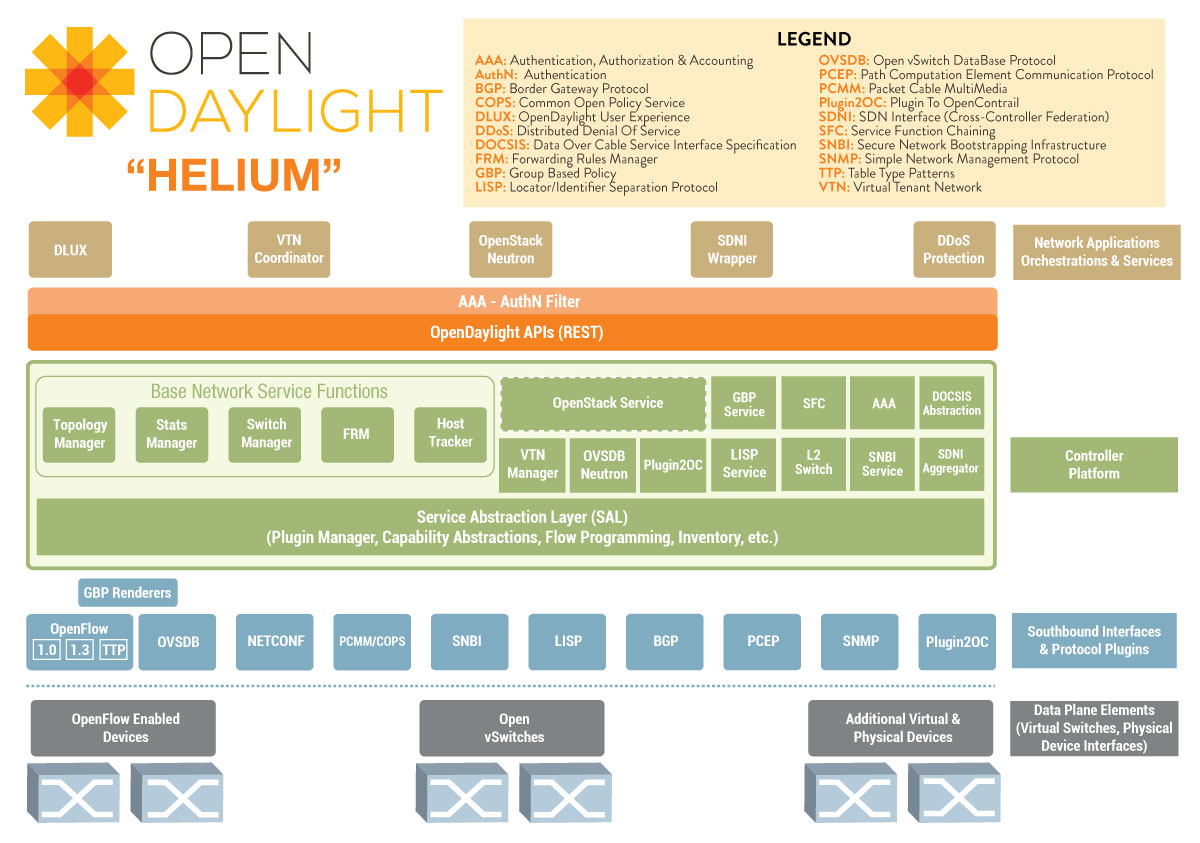
\includegraphics[width=15cm]{img/odl-technologies-01.png}
   \caption{OpenDaylight Architecture Diagram}
   \label{fig:odl_tech_diagram}
 \end{center}
 \end{figure}
\end{center}
OpenDaylight, as shown in previous figure, has been designed on a modular and pluggable basis. Main component of the project is a flexible controller platform, which is considered to be the core component. \textbf{This controller is implemented strictly in software and is contained within its own Java Virtual Machine (JVM)~\cite{Java}}. Having some disadvantages, \textbf{Java has been selected as the core component programming language to achieve the wider target users}, as it is known that Java can be deployed on a wide hardware and operating system platforms.\\
\\
The controller exposes open northbound APIs which are used by applications. OpenDaylight supports the \textbf{OSGi framework} and bidirectional \textbf{Representational State Transfer (REST)}~\cite{REST} for the northbound API. By using both technologies a \textbf{complete scope is provided}, as, while the OSGi framework is used for applications that will run in the same address space as the controller, the REST (web based) API is used for applications that do not run in the same address space (or even necessarily on the same machine) as the controller.\\
\\
The \textbf{business logic and algorithms reside in the applications}. Controller is used by the application to \textbf{gather network intelligence, run algorithms and perform analytics}. Apart from this, \textbf{controller is operated by applications to orchestrate the new rules, if any, throughout the network}.\\
\\
Apart from being multi-platform designed and being easily scalable, \textbf{extensibility} is one of the main characteristics of OpenDaylight project. \textbf{Controller} has been implemented \textbf{to be upgraded by dynamically pluggable modules} that can be added to perform required network tasks. There are a series of base network services to perform different basic tasks, as understanding what devices are contained within the network, capabilities of each of the components, monitorization or statistics retrieval. Besides this, for enhanced SDN functionality, platform oriented services and other extensions can also be inserted into the controller platform.\\
\\
The \textbf{southbound interface is capable of supporting multiple protocols (as separate plugins), e.g. OpenFlow 1.0, OpenFlow 1.3, BGP-LS, etc}. Service Abstraction Layer (SAL), has been designed for these modules to be dynamically linked into. The \textbf{SAL exposes device services to which the modules north of it are written, determining how to fulfill the requested service}, irrespective of the underlying protocol used between the controller and the network devices.\\
\\
One of the most exciting aspects of the OpenDaylight Project is that its components and technologies continue evolving based on the contributions of its developer community, favored by its extensible and modular design.

\section{OpenDaylight Projects}
\label{chap:odltech_projects}
After technical overview presentation ~\ref{chap:odltech_overview}, an analysis of the different technologies involved on OpenDaylight project development is performed on this chapter. To start with, it has already been mentioned that \textbf{OpenDaylight is structured in different projects that handle different software features provided}. Being the controller the main project of OpenDaylight, there is a complete set of projects to perform different tasks, provide different features to applications through Nortbound API and communicate over different protocols through the Southbound (SB) API.\\
\\
OpenDaylight project is in turn a set of different projects that have been contributed to a common platform, in order to achieve an homogeneous ecosystem around SDN and NFV technologies. Some of the projects are focused on a particular feature (i.e.:security). Meanwhile, other projects are based on developing or enhancing a Network Protocol (i.e.:OpenFlow). There are also another kind of projects that focuses on actions to accomplish for the correct evolution of the project, such as Documenation or Integration projects. In this section, OpenDaylight's project will be enumerated and briefly described, in order to increase the knowledge of each of the different pillars on which the project is sustained. It must be remarked that all of the information is available on the OpenDaylight Wiki~\cite{OpenDaylightWiki}:
\begin{enumerate}
\item{\textbf{AAA Service}}~\cite{OpenDaylightWikiAAA}. AAA project is aimed to provide \textbf{Authentication, Authorization and Accounting in OpenDaylight project}. On the one hand, Authentication allows managing users permissions to access the platform in a token/claim-basis, with support of authentication methods such as OAuth, SAML or Keystone, among others. On the other hand, Authorization mechanism allows determining which part of the SDN controllers can be used and/or administered by a particular user. Last, but not least, authentication provide features for all accesses to be recorded and queryable for various purposes such as billing, analysis, diagnostics or security audit.
\item{\textbf{Affinity Metadata Service}}~\cite{OpenDaylightWikiAffinity}. The Affinity service provides an API to allow applications and controller itself to create and share an abstract networking topology, independent to the infrastructure needs and preferences. The term \textbf{affinity describes the nature of “conversations” across the networking infrastructure and their participants}. The Affinity API allows intent to be specified in application and service terms independent of how and where the communicating workloads attach to the network, with no details of forwarding devices, vendors or technologies included. \textbf{This can enable users to, for example, customize the behavior of virtual networks to better support their applications without knowing anything about bridges, routers, VLANs or tunnels}. In the end, the \textbf{affinity} concept is based on a layered architectural model in which intelligent controllers dynamically provision data center network infrastructure to satisfy workload affinities, as directed by external applications.
\item{\textbf{BGP-LS/PCEP}}~\cite{OpenDaylightWikiBGP}. BGP/PCEP protocol project aims to provide Java-based implementation of Border Gateway Protocol (BGP)~\cite{BGP} and Path Computation Element Protocol (PCEP)~\cite{PCEP}. By enabling OpenDaylight platform to utilize more standardized ways of talking to the underlying network, it will be deployed in a wider variety of scenarios. \textbf{BGP is the core protocol holding together the Internet in its current shape and form}, while \textbf{PCEP} was designed for offloading optimal path computation. It is also remarkable the fact of the availability of Open Source Network Protocols software implementation, and BGP-LS/PCEP is aimed also to empower this fact.
\item{\textbf{Controller}}~\cite{OpenDaylightWikiController}. OpenDaylight Controller is, no doubt, the \textbf{main project} inside project's ecosystem. OpenDaylight's SDN Controller provides the ability to \textbf{deploy software to control the network gear and redeploy as needed}. The main goal within this project is to have a modular Controller with a well published Northbound API for network Applications to write towards while utilizing SB protocols such as OpenFlow to communicate with supported downstream network nodes.
\begin{center}
 \begin{figure}[H]
 \begin{center}
   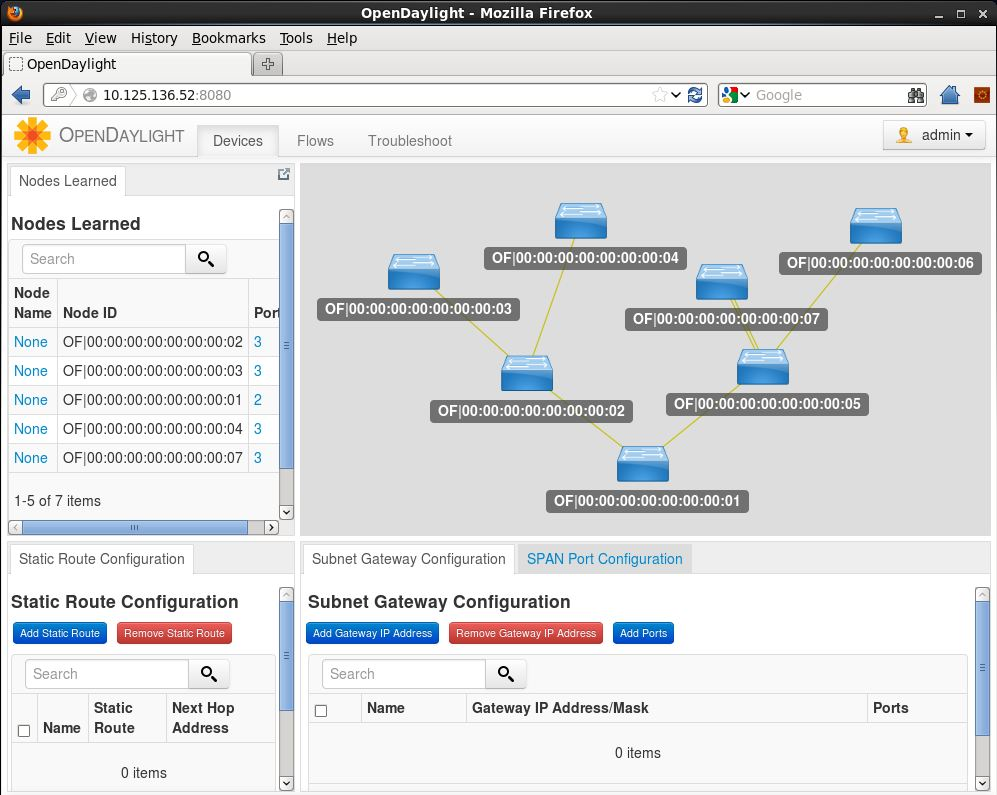
\includegraphics[width=15cm]{img/odl-controller-00.png}
   \caption{OpenDaylight Controller}
   \label{fig:odl_tech_diagram}
 \end{center}
 \end{figure}
\end{center}
Apart from detailed characteristics, the Controller provides interfaces to third party applications, such as \textbf{OpenStack Neutron} module, or advanced features such as \textbf{clustering, auditing and monitoring}.
\item{\textbf{dlux - openDayLight User eXperience}}~\cite{OpenDaylightWikiDlux}. This project focuses on OpenDaylights user experience. The latest (current) version uses a JavaScript based Single-Page-Application using AngularJS, running on NodeJS.
\item{\textbf{Documentation Project}}~\cite{OpenDaylightWikiDoc}. This vertical group aims to build the content infrastructure, improve the user content for the various OpenDaylight projects and ensure continued quality in the content.
\item{\textbf{Defense4All}}~\cite{OpenDaylightWikiDefense4All}. SDN application for detecting and mitigating Distributed Denial of Service (DDoS) attacks. By communicating with OpenDaylight Controller via north-bound REST API, performs tasks such as \textbf{monitoring behavior of protected traffic} and \textbf{diverting attacked traffic to selected Attack Mitigation Systems (AMSs)}.
\item{\textbf{Dynamic Resource Reservation}}~\cite{OpenDaylightWikiReservation}. Reservation application provides end to end multi-layer provisioning. \textbf{Reservation application focuses on flexible provisioning based on information such as latency, bandwidth or any other networking parameter involved in an end to end communication}.
\item{\textbf{Group Policy Plugin Project}}~\cite{OpenDaylightWikiGroupPolicy}. Currently, the project is in the early stages. The main aim of this project is to \textbf{separate applicatoin connectivity requirements and underlaying details of network infrastructure} via an application-centric policy model.
\item{\textbf{Integration Group}}~\cite{OpenDaylightWikiIntegration}. This project is more a infrastructure project that tries to coordinate and drive \textbf{integration and test efforts to achieve a successful OpenDaylight release}. To achieve this mission, tasks such as developing a test strategy, perform continous system integration test plan or develop and mantain an automated test framework are responsibilities of this project.
\item{\textbf{L2 Switch}}~\cite{OpenDaylightWikiL2Switch}. This project tries to separate out the Layer 2 specific handling code into a separate layer, creating several reusable services, by providing some generic L2 services, such as \textbf{Packet Handling}, \textbf{Address Tracking} or \textbf{Path Computation Services} . Depending on the Plugins loaded, Controller can contain certain packet handling/forwarding behavior with the ARPHandlers, Host Trackers, Simple Forwarders, etc.
\item{\textbf{LISP Flow Mapping}}~\cite{OpenDaylightWikiLISP}. The aim of this project is to enable LISP protocol~\cite{LISP} inside OpenDaylight. LISP is a network-layer-based protocol that enables separation of IP addresses into two new numbering spaces: Endpoint Identifiers (EIDs) and Routing Locators (RLOCs). This technology provides a flexible map-and-encap framework that \textbf{can be used for overlay network applications, such as data center network virtualization, and Network Function Virtualization (NFV)}.
\item{\textbf{Open DOVE}}~\cite{OpenDaylightWikiOpenDove}. Open Distributed Overlay Virtual Ethernet (OpenDOVE) project is a network virtualization platform with a full control plane implementation for OpenDaylight and \textbf{data plane based on OpenvSwitch}~\cite{OVS}. DOVE is, in turn,  a network virtualization platform that provides isolated multi-tenant networks on any IP network in a virtualized data center, providing each tenant with a virtual network abstraction providing layer-2 or layer-3 connectivity and the ability to control communication using access control policies.
\item{\textbf{OpenFlow Plugin}}~\cite{OpenDaylightWikiOpenFlowPlugin}. OpenFlow~\cite{OpenFlow} is a vendor-neutral standard communications interface defined to enable interaction between the control and forwarding layers of an SDN architecture. \textbf{The OpenFlow plugin project intends to develop a plugin to support implementations of the OpenFlow specification} as it develops and evolves. Specifically the project will continue to provide support for the existing OpenFlow 1.0 implementation, developing a plugin aiming to support OpenFlow 1.3.x, and further supporting subsequent OpenFlow specifications.
\item{\textbf{OpenFlow Protocol Library}}~\cite{OpenDaylightWikiOpenFlowLib}. This project provides a library that mediates communication between OpenDaylight controller and hardware devices supporting \textbf{OpenFlow}~\cite{OpenFlow}. Primary goal is to \textbf{provide a communication channel to the user in order to provide a mechanism for managing network hardware devices}.
\item{\textbf{OpFlex Implementation Project}}~\cite{OpenDaylightWikiOpenFlowLib}. This project consist of the implementation of the OpFlex protocol, tother with an OpenFlex SB plugin and Policy Agent to implement functionality of OpenFlex~\cite{OpFlex}, an architecture that provides a distributed control system based on a declarative policy information model.
\item{\textbf{OVSDB Open vSwitch Database Integration Project}}~\cite{OpenDaylightWikiOpFlex}. The OVSDB Plugin project tries to accomplish the implementation of the \textbf{Open vSwitch Database management protocol}~\cite{OVSDB}. The project consists of a library, along with various plugin usages, that allows configuration of vSwitches through southbound API.
\item{\textbf{OSCP Project}}~\cite{OpenDaylightWikiOSCP}. The OpenDaylight SDN Controller Platform (OSCP) is the \textbf{network application platform that provides unified network intelligence, enterprise-class scalability and high availability, and a platform to deploy a wide range of network applications}. The OSCP controller provides the centralized control plane tier in the three-tier Open SDN architecture. While OSCP is logically centralized, the controller is installed on multiple controller-nodes for redundancy and scale.
\item{\textbf{PacketCable PCMM Project}}~\cite{OpenDaylightWikiPacketCable}. Packet Cable MultiMedia (PCMM)~\cite{PCMM} provides an \textbf{interface to control and management service flow for Cable Modem Termination System (CMTS) network elements}. A service flow constitute a data path between a CMTS and a subscriber's cable modem (CM) guaranteed application specific quality of service (QoS), known as Dynamic Quality of Service (DQoS). PCMM offers the ability to deliver new services using existing cable infrastructure. \textbf{DOCSIS}~\cite{DOCSIS} encapsulation according to the standard has been introduced in OpenDaylight to achieve abstraction of this encapsulation type.
\item{\textbf{Secure Network Bootstrapping Infrastructure (SNBI) project}}~\cite{OpenDaylightWikiSNBI}.  The Secure Network Bootstrapping Infrastructure (SNBI) project is aimed to \textbf{perform securely and automatically the bring up of an integrated set of network devices and controllers}. SNBI devices and controllers automatically discover each other, get an IP-address assigned, and establish secure IP connectivity.
\item{\textbf{Service Function Chaining}}~\cite{OpenDaylightWikiSNMP}. Service Function Chaining provides the ability to define an ordered list of a network services (firewalls, load balancers, routers). These service are then linked together in the network to create a service chain. \textbf{This project provides the infrastructure (chaining logic, APIs) needed to provision a service chain in the network and an end-user application for defining such chains}.
\item{\textbf{SNMP4SDN}}~\cite{OpenDaylightWikiTTP}. This project has been proposed to develop a Simple Network Management Protocol \textbf{(SNMP) southbound plugin to control underlying devices supporting SNMP}, using off-the-shelf commodity Ethernet switch. In addition to SNMP support, this plugin will provide certain capabilities to manage configurations that can only be accessed via CLI, e.g. ACL or disabling flooding, since such configurations are necessary for using Ethernet switches for SDN.
\item{\textbf{Table Type Patterns (TTPs)/Negotiable Datapath Models (NDMs)}}~\cite{OpenDaylightWiki}. Table Type Patterns (TTPs) are the first tangible output from the ONF's Forwarding Abstractions Working Group (FAWG). The goal is to \textbf{allow for an OpenFlow controller and OpenFlow switch to agree on a set of functionality}, and help managing the increased diversity made possible with OpenFlow versions 1.1+.
\item{\textbf{Toolkit Project}}~\cite{OpenDaylightWikiToolkit}. One of the concerns in OpenDaylight was the consistent feedback received from developers about the complexity in developing apps for OpenDaylight. OpenDaylight Toolkit is a \textbf{framework to enabled developers to easily develop applications on top of the OpenDaylight controller}. The main mission of the project is to be infrastructure independent and allow developers to develop application on top of multiple platforms.
\item{\textbf{Virtual Tenant Network (VTN)}}~\cite{OpenDaylightWikiVTN}. OpenDaylight Virtual Tenant Network (VTN) is an \textbf{application that provides multi-tenant virtual network on an SDN controller}. The network is designed on VTN, as \textbf{VTN basically allows the users to define the network with L2/L3 network look and feel}. Once network is designed, it will automatically be mapped into underlying physical network, and then configured on the individual switch leveraging SDN control protocol.
\item{\textbf{YANG Tools}}~\cite{OpenDaylightWikiYANG}. Last, but not least, YANG Tools is a infrastructure project aiming to develop \textbf{necessary tooling and libraries providing support of NETCONF}~\cite{NETCONF} and \textbf{YANG}~\cite{YANG} for Java (JVM-language based) projects and applications. The project aims generic functionality related to the YANG, that should not be a part of Controller project, and should live in separate project to be reused by other applications and parties without directly depending on Controller.
\end{enumerate}

\section{OpenDaylight Source Code}
\label{chap:odltech_source_code}
It is important to analyze \textbf{programming languages involved}, in order to identify which are the main software development languages used in both the core controller and the different plugins and other subprojects available on the project, as programming languages usage is a key aspect to analyze the technical constraints.\\
\\
As previously described, OpenDaylight project is composed in turn of a subset of projects that allow achieving a complete platform to act as SDN Controller as well as provide NFV functionalities through an Open Source software basis.\\
\\
OpenDaylight's software source code is splitted taking into account different previously described projects existence, and can be retrieved from different GIT repositories (one per project), described in below table:
\begin{table}[H]
\footnotesize
\begin{center}
\begin{tabular}{|p{6cm}|l|}
\hline
\textbf{Project} & \textbf{Git Repository} \\ \hline
AAA Service & https://git.opendaylight.org/gerrit/p/aaa.git \\ \hline
Affinity Metadata Service & https://git.opendaylight.org/gerrit/p/affinity.git \\ \hline
BGP-LS/PCEP & https://git.opendaylight.org/gerrit/p/bgpcep.git \\ \hline
Controller & https://git.opendaylight.org/gerrit/p/controller.git \\ \hline
dlux - openDayLight User eXperience & https://git.opendaylight.org/gerrit/p/dlux.git \\ \hline
Documentation Project & https://git.opendaylight.org/gerrit/p/docs.git \\ \hline
Defense4All & https://git.opendaylight.org/gerrit/p/defense4all.git \\ \hline
Dynamic Resource Reservation  & https://git.opendaylight.org/gerrit/p/reservation.git \\ \hline
Group Policy Plugin Project & https://git.opendaylight.org/gerrit/p/groupbasedpolicy.git \\ \hline
Integration Group & https://git.opendaylight.org/gerrit/p/integration.git \\ \hline
L2 Switch & https://git.opendaylight.org/gerrit/p/l2switch.git \\ \hline
LISP Flow Mapping & https://git.opendaylight.org/gerrit/p/lispflowmapping.git \\ \hline
Open DOVE & https://git.opendaylight.org/gerrit/opendove.git \\ \hline
OpenFlow Plugin & https://git.opendaylight.org/gerrit/p/openflowjava.git \\ \hline
OpenFlow Protocol Library & https://git.opendaylight.org/gerrit/p/openflowplugin.git \\ \hline
OpFlex Implementation Project & https://git.opendaylight.org/gerrit/p/opflex.git \\ \hline
OVSDB Open vSwitch Database Integration Project & https://git.opendaylight.org/gerrit/p/ovsdb.git \\ \hline
OSCP Project & https://git.opendaylight.org/gerrit/p/net-virt-platform.git \\ \hline
PacketCable PCMM Project & https://git.opendaylight.org/gerrit/p/packetcable.git \\ \hline
Secure Network Bootstrapping Infrastructure (SNBI) project & https://git.opendaylight.org/gerrit/p/snbi.git \\ \hline
Service Function Chaining & https://git.opendaylight.org/gerrit/p/sfc.git \\ \hline
SNMP4SDN  & https://git.opendaylight.org/gerrit/p/snmp4sdn.git \\ \hline
Table Type Patterns (TTPs)/Negotiable Datapath Models (NDMs) & https://git.opendaylight.org/gerrit/p/ttp.git \\ \hline
Toolkit Project & https://git.opendaylight.org/gerrit/p/toolkit.git \\ \hline
Virtual Tenant Network (VTN) & https://git.opendaylight.org/gerrit/p/vtn.git \\ \hline
YANG Tools & https://git.opendaylight.org/gerrit/p/yangtools.git \\ \hline
\end{tabular}
\end{center}
\caption{OpenDaylight projects' repositories}
\label{tab:projectgitrepos}
\end{table}
Previous repositories collection contain all the source code composing OpenDaylight software. It has been also clarified that the core component, the \textbf{controller, has been implemented in Java}. But, regarding source code, programming languages used and other software stuff, is worth considering a set of questions: how wide is OpenDaylight software? Are there other programming languages used in the project apart from Java? Which is the most used programming language?\\
\\
To start with, it must be clarified that SLOCCount~\cite{SLOCCount} has been used in order to perform different measures across the different repositories. By using this tool, next measures have been obtained:
\begin{itemize}\itemsep0pt
\item{\textbf{Source Lines Of Code (SLOC)}}. This tool allows counting the total amount of lines of code existing on the project. This is a first aproximation to measure the complexity of the project and different subprojects.
\item{\textbf{Programming Languages Usage and Classification}}. SLOCCount also provides a mechanism to classify the total percent usage of each of the programming languages in the the whole source code of the project.
\end{itemize}
Using SLOCCount is frankly simple, as it only has to be executed on the directory where all the code has been retrieved:

\begin{verbatim}
$ sloccount .
Creating filelist for aaa
Creating filelist for affinity
Creating filelist for bgpcep
Creating filelist for controller
...
Creating filelist for yangtools

SLOC    Directory       SLOC-by-Language (Sorted)
661838  vtn             cpp=349960,java=192289,ansic=80272,
                        python=17402, perl=11928,xml=8904,
                        sh=964,asm=119
289437  controller      java=250524,xml=37816,sh=772,jsp=325
142681  oscp            java=98499,python=42727,xml=1075,sh=380
99718   opendove        ansic=67487,python=23998,java=7260,xml=817,
                        sh=156
82770   yangtools       java=75792,xml=6978
59026   defense4all     java=56122,xml=2010,sh=461,perl=356,
                        python=77
55431   bgpcep          java=43460,xml=7586,python=4385
47232   openflowplugin  java=37604,xml=7486,python=2140,sh=2
37232   sdninterfaceapp java=33954,xml=3278
33577   ovsdb           java=28162,xml=4840,sh=421,python=154
32348   dlux            xml=32086,java=262
27003   openflowjava    java=25704,xml=1299
23443   snbi            ansic=18796,java=3357,xml=1168,sh=72,
                        python=50
22672   opflex          ansic=19412,python=2844,sh=416
20032   snmp4sdn        java=18171,xml=1861
16138   groupbasedpolicy java=14532,xml=1228,python=378
15627   packetcable     java=13780,xml=1248,python=455,sh=144
15436   integration     xml=9377,python=3851,sh=2208
14479   lispflowmapping java=11384,xml=3095
11415   aaa             java=7977,xml=2925,sh=513
11311   toolkit         java=5365,xml=5254,jsp=499,sh=193
11167   l2switch        java=8190,xml=2977
9567    sfc             java=5902,xml=3223,python=417,sh=25
8375    docs            xml=8375
8206    affinity        java=5128,xml=1949,python=1085,sh=44
3659    tcpmd5          java=2161,xml=1205,ansic=293
1752    reservation     xml=1752
1567    ttp             xml=892,java=437,python=238
910     odlparent       xml=910

Totals grouped by language (dominant language first):
java:        946016 (53.63%)
cpp:         349960 (19.84%)
ansic:       186260 (10.56%)
xml:         161614 (9.16%)
python:      100201 (5.68%)
perl:         12284 (0.70%)
sh:            6771 (0.38%)
jsp:            824 (0.05%)
asm:            119 (0.01%)

Total Physical Source Lines of Code (SLOC) = 1,764,049
Development Effort Estimate, Person-Years  = 512.70
Basic COCOMO model, Person-Months = 2.4 * (KSLOC**1.05))
Schedule Estimate, Years (Months) = 5.74 (68.83)
 (Basic COCOMO model, Months = 2.5 * (person-months**0.38))
Estimated Average Number of Developers = 89.39
Total Estimated Cost to Develop = $ 69,259,253
 (average salary = $56,286/year, overhead = 2.40).
SLOCCount, Copyright (C) 2001-2004 David A. Wheeler
\end{verbatim}
Taking previous data into consideration, some graphics can be created to show the different measures performed \footnote{Software Source Code retrieval performed on October 4th, 2014} on a more representative way. To start with, figure below shows the distribution percentage from programming languages perspective:
\begin{center}
 \begin{figure}[H]
 \begin{center}
   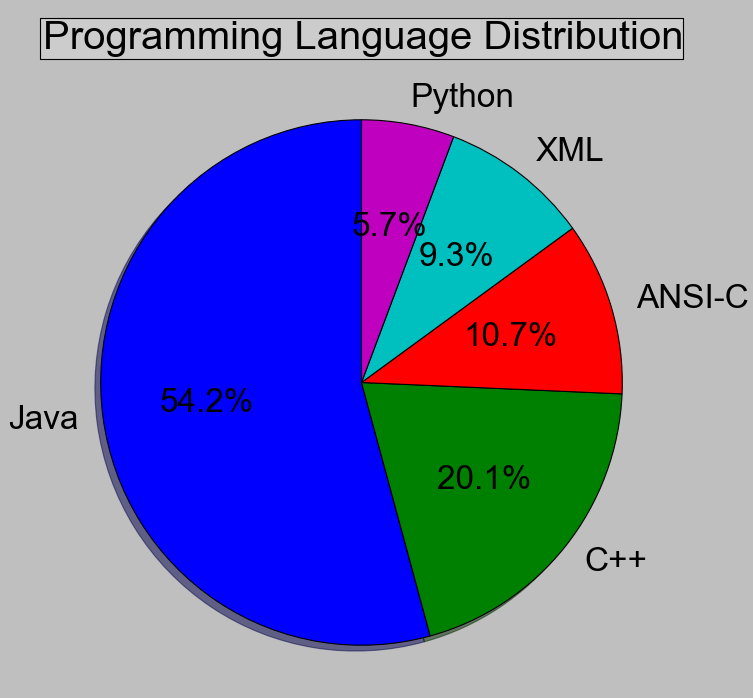
\includegraphics[width=15cm]{img/sloc-distritbution-01.png}
   \caption{OpenDaylight Programming Language Distribution}
   \label{fig:odl_prog_dist_diagram}
 \end{center}
 \end{figure}
\end{center}
As shown before, \textbf{Java, C++ and ANSI-C} are predominant programming languages used inside OpenDaylight project. 85\% of the code is written in one of these programming languages, while \textbf{15\% of the remaining code is written in well-known programming languagues, such as Python or XML}\footnote{XML is rather a markup language, but has been considered a programming language to homogenize data dumped by SLOCCount tool}. It must be highlighted that \textbf{C, Java and C++ are among the most used five programming languages in 2014, while Python holds the eigth place}, according to the TIOBE Index~\cite{TiobeIndex}.\\
\\
It is also interesting to classify the different existing projects distribution taking into account Lines Of Code (LOC). First, with a very simple calculation of the total lines of code in the project, it results on OpenDaylight project to have a \textbf{total of 1764049 LOCs}. This way, calculation of the percentage of the total code used by each project can be performed easily. Next table summarizes the output of the previous command:
\begin{table}[H]
\footnotesize
\begin{center}
\begin{tabular}{|l|l|l|}
\hline
\textbf{Project} & \textbf{LOCs} & \textbf{LOCs percentage} \\ \hline
vtn               & 661838 & 37.51\% \\ \hline
controller        & 289437 & 16.40\% \\ \hline
oscp              & 142681 &  8.08\% \\ \hline
opendove          & 99718  &  5.65\% \\ \hline
yangtools         & 82770  &  4.69\% \\ \hline
defense4all       & 59026  &  3.34\% \\ \hline
bgpcep            & 55431  &  3.14\% \\ \hline
openflowplugin    & 47232  &  2.67\% \\ \hline
sdninterfaceapp   & 37232  &  2.11\% \\ \hline
ovsdb             & 33577  &  1.90\% \\ \hline
dlux              & 32348  &  1.83\% \\ \hline
openflowjava      & 27003  &  1.53\% \\ \hline
snbi              & 23443  &  1.32\% \\ \hline
opflex            & 22672  &  1.28\% \\ \hline
snmp4sdn          & 20032  &  1.13\% \\ \hline
groupbasedpolicy  & 16138  &  0.91\% \\ \hline
packetcable       & 15627  &  0.88\% \\ \hline
integration       & 15436  &  0.87\% \\ \hline
lispflowmapping   & 14479  &  0.82\% \\ \hline
aaa               & 11415  &  0.64\% \\ \hline
toolkit           & 11311  &  0.64\% \\ \hline
l2switch          & 11167  &  0.63\% \\ \hline
sfc               & 9567   &  0.54\% \\ \hline
docs              & 8375   &  0.47\% \\ \hline
affinity          & 8206   &  0.46\% \\ \hline
reservation       & 1752   &  0.09\% \\ \hline
ttp               & 1567   &  0.08\% \\ \hline
\end{tabular}
\end{center}
\caption{OpenDaylight projects' LOC distribution}
\label{tab:projectlocdistribution}
\end{table}
Previous table has been obtained by using some advance text processing command, such as \textbf{gawk}~\cite{GAWK}, and dumping the output of the lines of code distribution to a file (i.e.:loc.txt), it is quite easy to calculate percent of lines of code used by each of the subprojects, as shows next command:
\begin{verbatim}
$ cat loc.txt | grep ^[0-9] | awk {'print $1'} |
while read line; do echo "scale=2; ($line*100)/1764049" | bc
\end{verbatim}
Data retrieved can be plotted in a more representative way through a percent distribution Pie chart, as shown in next figure:
\begin{figure}[H]
 \begin{center}
   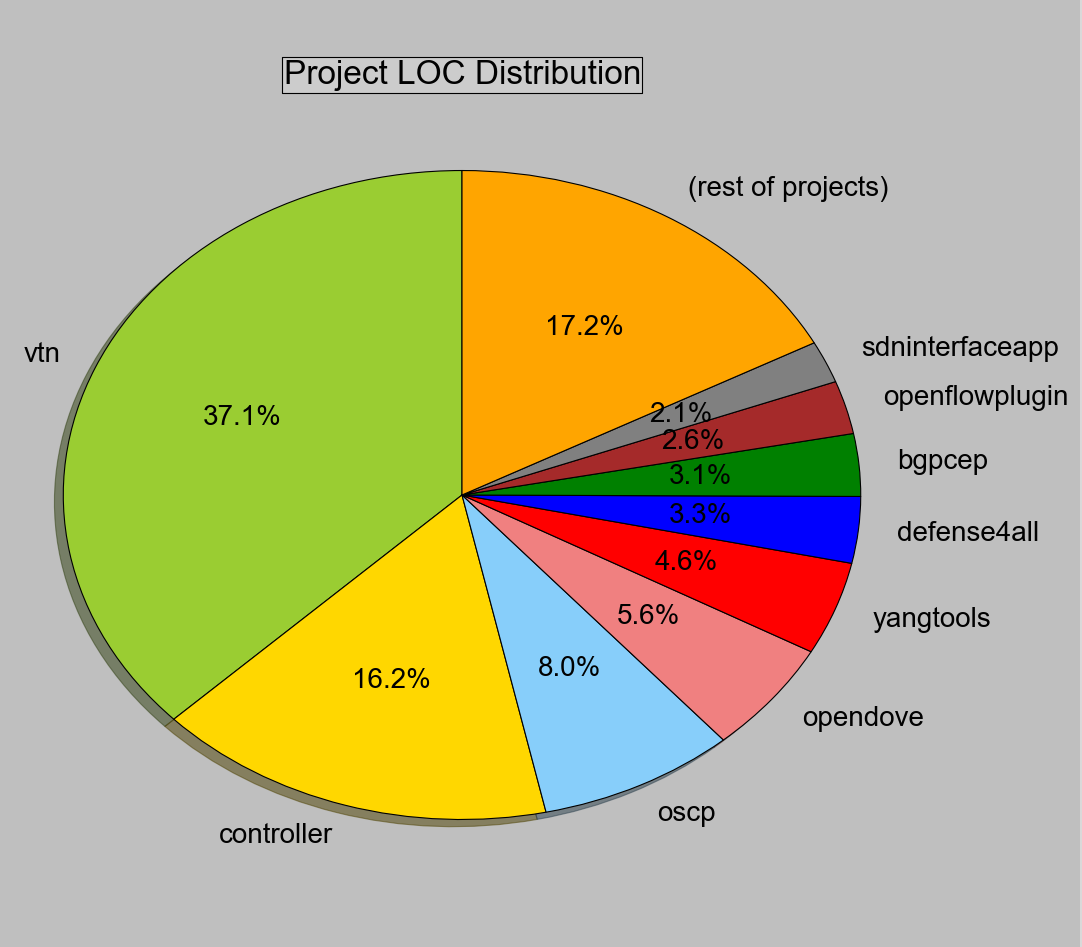
\includegraphics[width=15cm]{img/sloc-project-distritbution-02.png}
   \caption{OpenDaylight LOC based Project Distribution}
   \label{fig:odl_prog_loc_dist_diagram}
 \end{center}
\end{figure}

\section{Release Roadmap}
\label{chap:odltech_technologies}

Up to date, only two official releases of OpenDaylight have been released. Releases were named ``Hydrogen'' and ``Helium''. Initial version, called ``Hydrogen'', was released February 4th, 2014. This release was a first try by OpenDaylight group to achieve a SDN controller that could act as SDN/NFV controller. To do, not all the projects already available were included, but rather some of the most important which were, in turn, with such a maturity level to be included in a official release. Next table show modules on that first releaes:
\begin{center}
 \begin{figure}[H]
 \begin{center}
   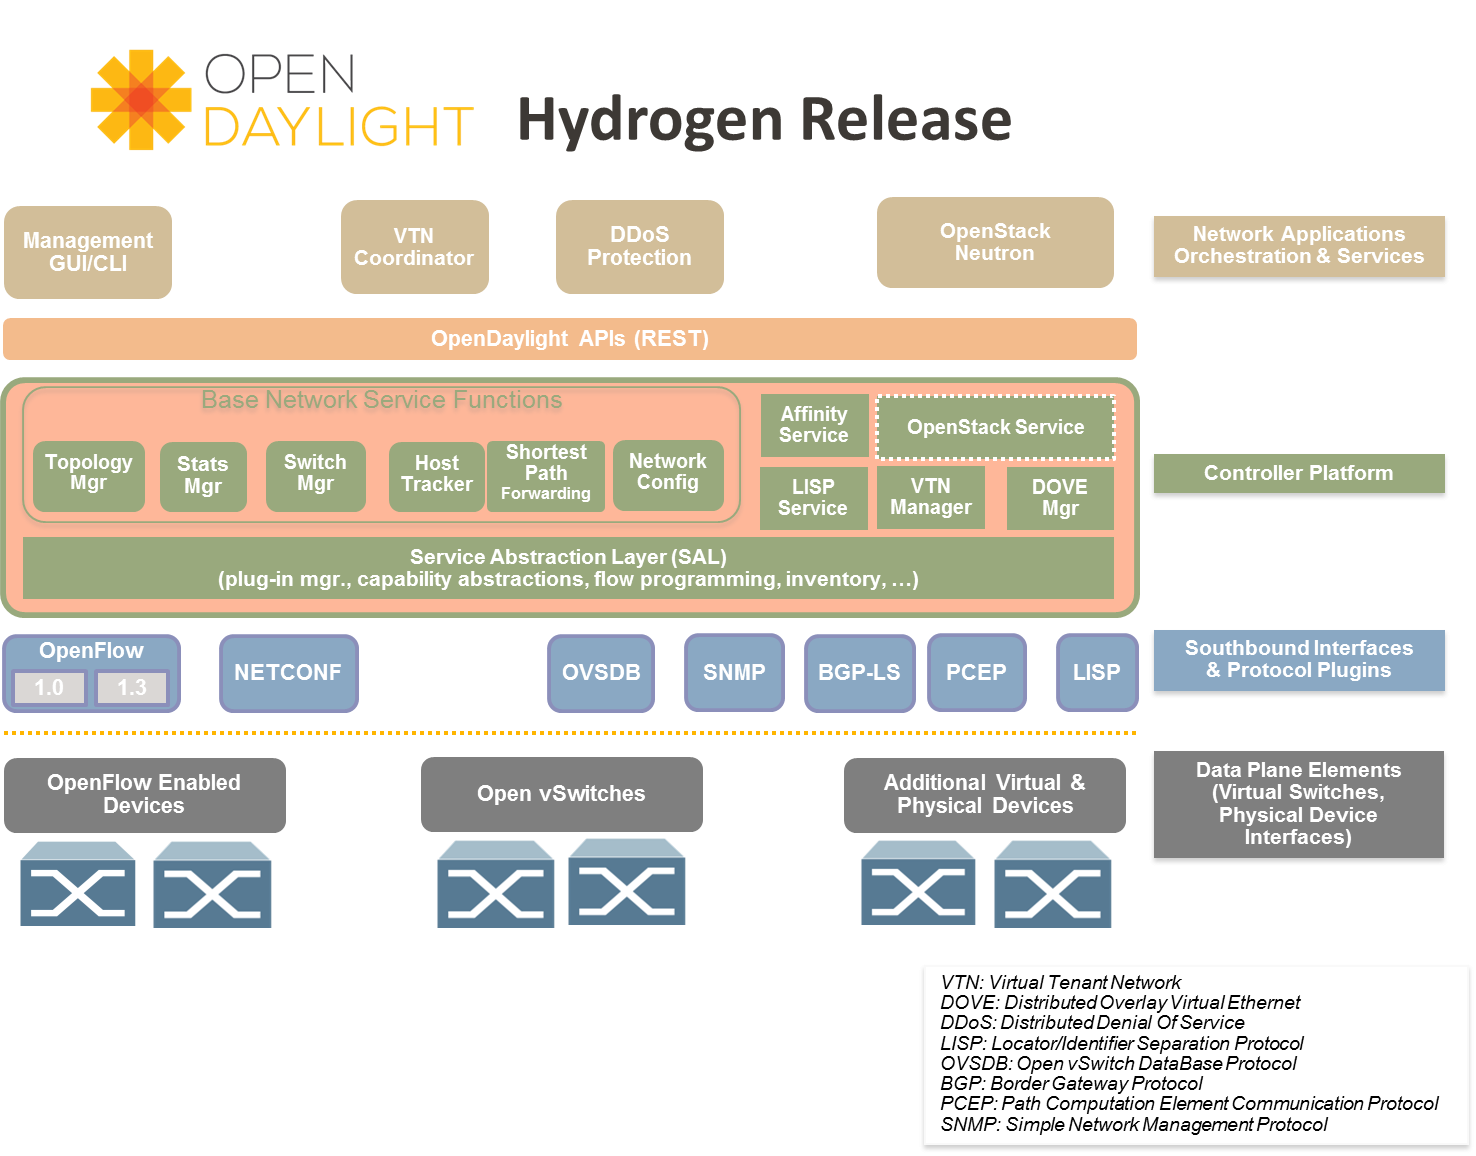
\includegraphics[width=15cm]{img/odl-technologies-00.png}
   \caption{OpenDaylight Hydrogen Architecture Diagram}
   \label{fig:odl_tech_diagram}
 \end{center}
 \end{figure}
\end{center}
Meanwhile, ``Helium'', the second final version of OpenDaylight, which was released September 29th, 2014, brought up to ten improvements and new features. Among them, next ones are remarkable:
\begin{enumerate}\itemsep0pt
\item{\textbf{New SB plugins}}. This way, enhanced communication to underlying hardware was introduced. Among the most important protocols introduced, next ones are to highlight:
\begin{itemize}\itemsep0pt
\item{OpenFlow TTP}
\item{PCMM}
\item{SNBI}
\end{itemize}
\item{\textbf{New features and services}}. Among new features and services introduced, next ones are found:
\begin{itemize}\itemsep0pt
\item{AAA}
\item{DOCSIS abstraction}
\item{SFC}
\item{L2 Switch}
\item{OVSDB Neutron}
\end{itemize}
\item{\textbf{New NB API}}. Last but not least, new NB API has also been added:
\begin{itemize}\itemsep0pt
\item{AuthN API}
\end{itemize}
\end{enumerate}
Next figure shows information about new features, services and APIs that have been incorporated in ``Helium'' release:
\begin{center}
 \begin{figure}[H]
 \begin{center}
   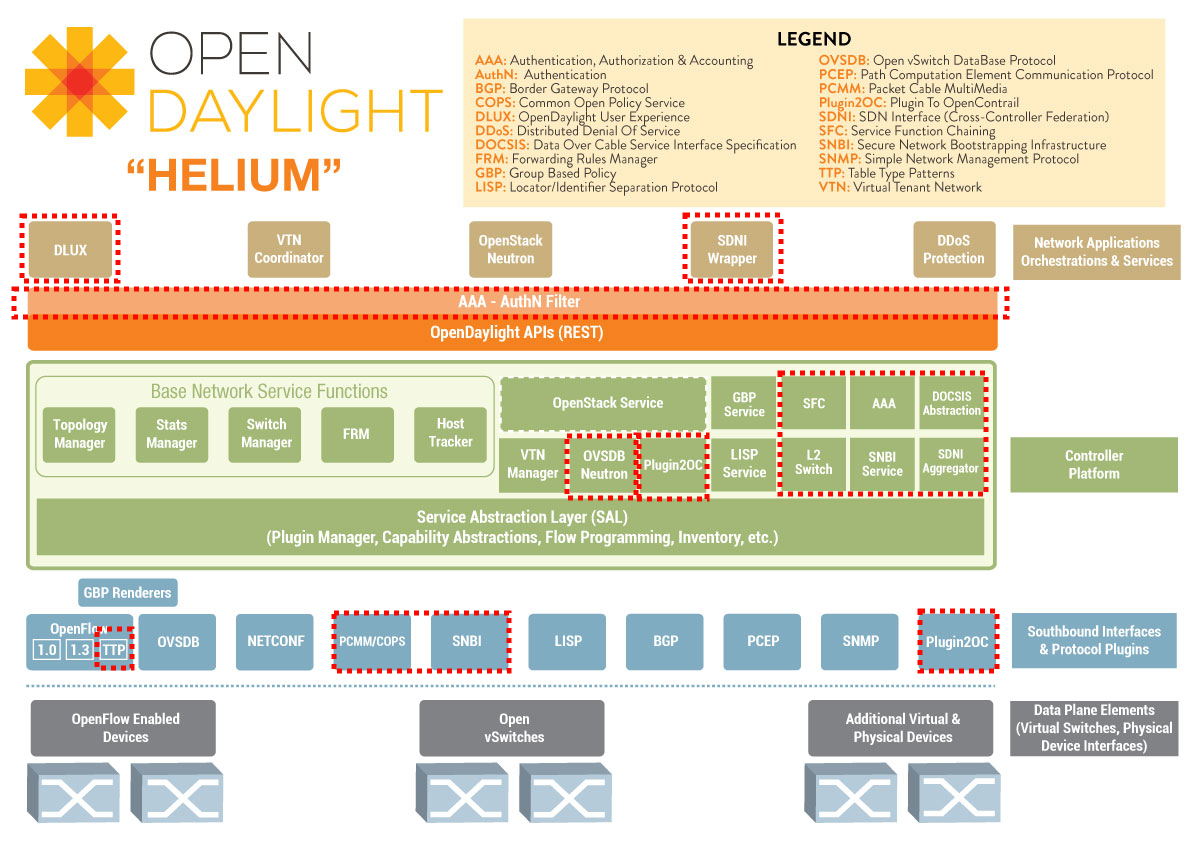
\includegraphics[width=15cm]{img/odl-technologies-02.png}
   \caption{OpenDaylight Helium New Features Diagram}
   \label{fig:odl_tech_helium_new_diagram}
 \end{center}
 \end{figure}
\end{center}
There is no available information about next releases to be considered. However, it is important to know about \textbf{Project Lifecycle}~\cite{OpenDaylightLifecycle} inside OpenDaylight. How are new projects introduced? Can anybody propose a project? What are steps and times needed for a project to be included in an official release?\\
\\
The most important aspect regarding new projects proposal is that \textbf{everybody can propose a new project}. Obviously, it has to be a project that results valid to the OpenDaylight project, and must be related to the technologies and features provided by it.\\
\\
Next figure shows the steps followed by a new project from the time it is proposed until it is included in the Core or Top Level projects, or it is Archived due to decissions taken inside the Community to make that project out of the scope of OpenDaylight:
\begin{center}
 \begin{figure}[H]
 \begin{center}
   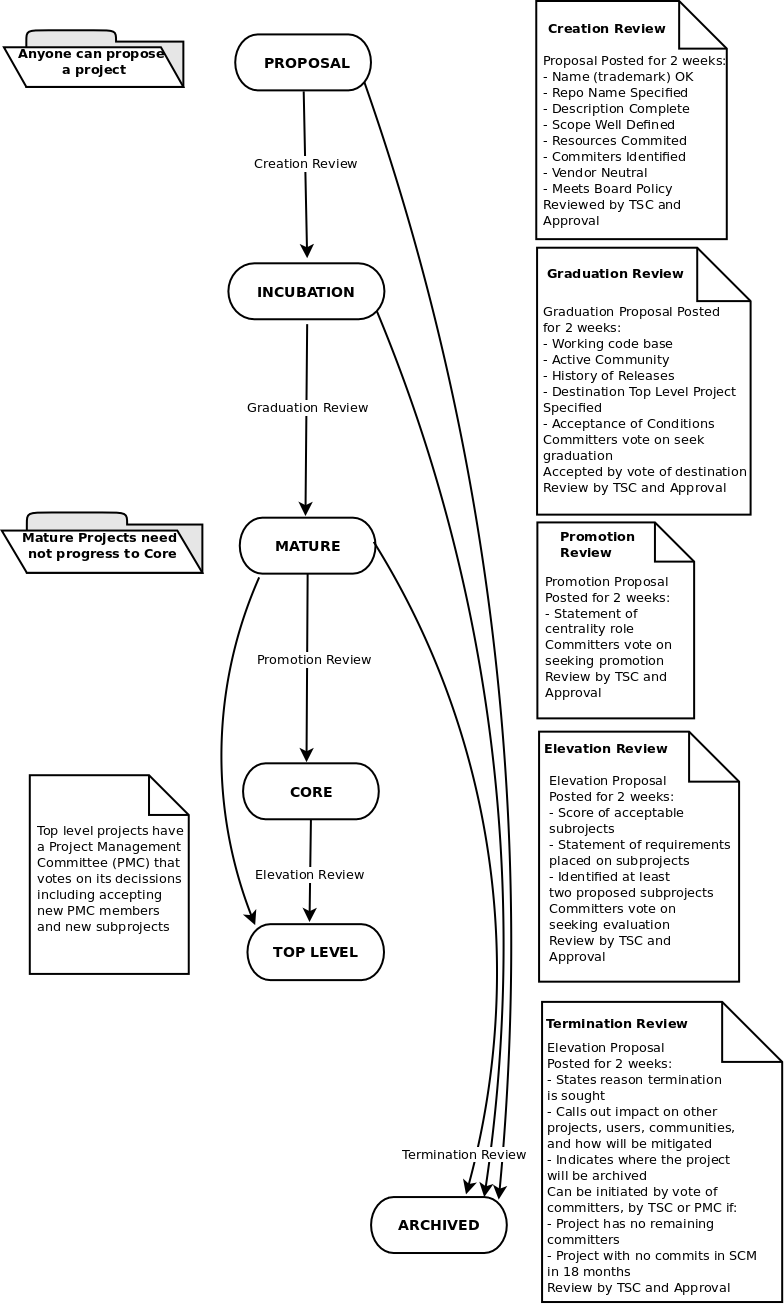
\includegraphics[width=14cm]{img/odl-proj-lifecycle-00.png}
   \caption{OpenDaylight Projects Life Cycle}
   \label{fig:odl_tech_proj_life_diagram}
 \end{center}
 \end{figure}
\end{center}

\section{Technnical Infrastructure}
\label{chap:odltech_infrastructure}

\section{Ease of...}
\label{chap:odltech_ease}

\chapter{OpenDaylight: Project Evaluation}
\label{chap:odlprojeval}

%%%%%%%%%%%%%%%%%%%%%%%%%%%%%%%%%%%%%%

\chapter{Conclusions}
\label{chap:conclusions}

%%%%%%%%%%%%%%%%
% Review goals and objectives

\section{Evaluation}
\label{sec:evaluation}

%%%%%%%%%%%%%%%%%%%%%%%%%%%%%%%%%%%%%%

Review goals and objectives

%%%%%%%%%%%

\section{Lessons learned}
\label{sec:lessons}

\subsection{Lesson 1}
\begin{itemize}
 \item Explain here what anybody may learn from this document
\end{itemize}

\subsection{What I learned}
\begin{itemize}
 \item Explain what you learned writing this document
\end{itemize}

\subsection{Knowledge and skills acquired in the M.Sc. studies that helped me on
this work}
\begin{itemize}
 \item You can go subject by subject, explained in which aspects helped
you to do/write this project
 \item Or just mention only the main aspects/subjects

\end{itemize}

\section{Future work}
\label{sec:future}

\subsection{More on...}

If there is any aspect that is not fully covered, explain how it could be
better covered.

\subsection{Other aspects}

See the section about ``Scope'' and explain here other aspects that you didn't
cover but it could be nice to work on.


\subsection{Other focuses}

For example study similar projects, or apply other tools to do the same work.

%%%%%%%%%%%%%%%%%%%%%%%%%%%%%%%%%%%%%
\appendix
\chapter{EPLv1.0}
\label{chap:appendix_eplv10}
Eclipse Public License - v 1.0\\
\\
THE ACCOMPANYING PROGRAM IS PROVIDED UNDER THE TERMS OF THIS ECLIPSE PUBLIC LICENSE ("AGREEMENT"). ANY USE, REPRODUCTION OR DISTRIBUTION OF THE PROGRAM CONSTITUTES RECIPIENT'S ACCEPTANCE OF THIS AGREEMENT.\\
\\
1. DEFINITIONS\\
\\
"Contribution" means:\\
\\
a) in the case of the initial Contributor, the initial code and documentation distributed under this Agreement, and\\
b) in the case of each subsequent Contributor:\\
i) changes to the Program, and
ii) additions to the Program;\\
where such changes and/or additions to the Program originate from and are distributed by that particular Contributor. A Contribution 'originates' from a Contributor if it was added to the Program by such Contributor itself or anyone acting on such Contributor's behalf. Contributions do not include additions to the Program which: (i) are separate modules of software distributed in conjunction with the Program under their own license agreement, and (ii) are not derivative works of the Program.\\
"Contributor" means any person or entity that distributes the Program.\\
"Licensed Patents" mean patent claims licensable by a Contributor which are necessarily infringed by the use or sale of its Contribution alone or when combined with the Program.\\
"Program" means the Contributions distributed in accordance with this Agreement.\\
"Recipient" means anyone who receives the Program under this Agreement, including all Contributors.\\
\\
2. GRANT OF RIGHTS\\
\\
a) Subject to the terms of this Agreement, each Contributor hereby grants Recipient a non-exclusive, worldwide, royalty-free copyright license to reproduce, prepare derivative works of, publicly display, publicly perform, distribute and sublicense the Contribution of such Contributor, if any, and such derivative works, in source code and object code form.\\
\\
b) Subject to the terms of this Agreement, each Contributor hereby grants Recipient a non-exclusive, worldwide, royalty-free patent license under Licensed Patents to make, use, sell, offer to sell, import and otherwise transfer the Contribution of such Contributor, if any, in source code and object code form. This patent license shall apply to the combination of the Contribution and the Program if, at the time the Contribution is added by the Contributor, such addition of the Contribution causes such combination to be covered by the Licensed Patents. The patent license shall not apply to any other combinations which include the Contribution. No hardware per se is licensed hereunder.\\
\\
c) Recipient understands that although each Contributor grants the licenses to its Contributions set forth herein, no assurances are provided by any Contributor that the Program does not infringe the patent or other intellectual property rights of any other entity. Each Contributor disclaims any liability to Recipient for claims brought by any other entity based on infringement of intellectual property rights or otherwise. As a condition to exercising the rights and licenses granted hereunder, each Recipient hereby assumes sole responsibility to secure any other intellectual property rights needed, if any. For example, if a third party patent license is required to allow Recipient to distribute the Program, it is Recipient's responsibility to acquire that license before distributing the Program.\\
\\
d) Each Contributor represents that to its knowledge it has sufficient copyright rights in its Contribution, if any, to grant the copyright license set forth in this Agreement.\\
\\
3. REQUIREMENTS\\
\\
A Contributor may choose to distribute the Program in object code form under its own license agreement, provided that:\\
\\
a) it complies with the terms and conditions of this Agreement; and\\
b) its license agreement:\\
i) effectively disclaims on behalf of all Contributors all warranties and conditions, express and implied, including warranties or conditions of title and non-infringement, and implied warranties or conditions of merchantability and fitness for a particular purpose;\\
ii) effectively excludes on behalf of all Contributors all liability for damages, including direct, indirect, special, incidental and consequential damages, such as lost profits;\\
iii) states that any provisions which differ from this Agreement are offered by that Contributor alone and not by any other party; and\\
iv) states that source code for the Program is available from such Contributor, and informs licensees how to obtain it in a reasonable manner on or through a medium customarily used for software exchange.\\
\\
When the Program is made available in source code form:\\
\\
a) it must be made available under this Agreement; and\\
b) a copy of this Agreement must be included with each copy of the Program.\\
Contributors may not remove or alter any copyright notices contained within the Program.\\
Each Contributor must identify itself as the originator of its Contribution, if any, in a manner that reasonably allows subsequent Recipients to identify the originator of the Contribution.\\
\\
4. COMMERCIAL DISTRIBUTION\\
\\
Commercial distributors of software may accept certain responsibilities with respect to end users, business partners and the like. While this license is intended to facilitate the commercial use of the Program, the Contributor who includes the Program in a commercial product offering should do so in a manner which does not create potential liability for other Contributors. Therefore, if a Contributor includes the Program in a commercial product offering, such Contributor ("Commercial Contributor") hereby agrees to defend and indemnify every other Contributor ("Indemnified Contributor") against any losses, damages and costs (collectively "Losses") arising from claims, lawsuits and other legal actions brought by a third party against the Indemnified Contributor to the extent caused by the acts or omissions of such Commercial Contributor in connection with its distribution of the Program in a commercial product offering. The obligations in this section do not apply to any claims or Losses relating to any actual or alleged intellectual property infringement. In order to qualify, an Indemnified Contributor must: a) promptly notify the Commercial Contributor in writing of such claim, and b) allow the Commercial Contributor to control, and cooperate with the Commercial Contributor in, the defense and any related settlement negotiations. The Indemnified Contributor may participate in any such claim at its own expense.\\
\\
For example, a Contributor might include the Program in a commercial product offering, Product X. That Contributor is then a Commercial Contributor. If that Commercial Contributor then makes performance claims, or offers warranties related to Product X, those performance claims and warranties are such Commercial Contributor's responsibility alone. Under this section, the Commercial Contributor would have to defend claims against the other Contributors related to those performance claims and warranties, and if a court requires any other Contributor to pay any damages as a result, the Commercial Contributor must pay those damages.\\
\\
5. NO WARRANTY\\
\\
EXCEPT AS EXPRESSLY SET FORTH IN THIS AGREEMENT, THE PROGRAM IS PROVIDED ON AN "AS IS" BASIS, WITHOUT WARRANTIES OR CONDITIONS OF ANY KIND, EITHER EXPRESS OR IMPLIED INCLUDING, WITHOUT LIMITATION, ANY WARRANTIES OR CONDITIONS OF TITLE, NON-INFRINGEMENT, MERCHANTABILITY OR FITNESS FOR A PARTICULAR PURPOSE. Each Recipient is solely responsible for determining the appropriateness of using and distributing the Program and assumes all risks associated with its exercise of rights under this Agreement , including but not limited to the risks and costs of program errors, compliance with applicable laws, damage to or loss of data, programs or equipment, and unavailability or interruption of operations.\\
\\
6. DISCLAIMER OF LIABILITY\\
\\
EXCEPT AS EXPRESSLY SET FORTH IN THIS AGREEMENT, NEITHER RECIPIENT NOR ANY CONTRIBUTORS SHALL HAVE ANY LIABILITY FOR ANY DIRECT, INDIRECT, INCIDENTAL, SPECIAL, EXEMPLARY, OR CONSEQUENTIAL DAMAGES (INCLUDING WITHOUT LIMITATION LOST PROFITS), HOWEVER CAUSED AND ON ANY THEORY OF LIABILITY, WHETHER IN CONTRACT, STRICT LIABILITY, OR TORT (INCLUDING NEGLIGENCE OR OTHERWISE) ARISING IN ANY WAY OUT OF THE USE OR DISTRIBUTION OF THE PROGRAM OR THE EXERCISE OF ANY RIGHTS GRANTED HEREUNDER, EVEN IF ADVISED OF THE POSSIBILITY OF SUCH DAMAGES.\\
\\
7. GENERAL\\
\\
If any provision of this Agreement is invalid or unenforceable under applicable law, it shall not affect the validity or enforceability of the remainder of the terms of this Agreement, and without further action by the parties hereto, such provision shall be reformed to the minimum extent necessary to make such provision valid and enforceable.\\
\\
If Recipient institutes patent litigation against any entity (including a cross-claim or counterclaim in a lawsuit) alleging that the Program itself (excluding combinations of the Program with other software or hardware) infringes such Recipient's patent(s), then such Recipient's rights granted under Section 2(b) shall terminate as of the date such litigation is filed.\\
\\
All Recipient's rights under this Agreement shall terminate if it fails to comply with any of the material terms or conditions of this Agreement and does not cure such failure in a reasonable period of time after becoming aware of such noncompliance. If all Recipient's rights under this Agreement terminate, Recipient agrees to cease use and distribution of the Program as soon as reasonably practicable. However, Recipient's obligations under this Agreement and any licenses granted by Recipient relating to the Program shall continue and survive.\\
\\
Everyone is permitted to copy and distribute copies of this Agreement, but in order to avoid inconsistency the Agreement is copyrighted and may only be modified in the following manner. The Agreement Steward reserves the right to publish new versions (including revisions) of this Agreement from time to time. No one other than the Agreement Steward has the right to modify this Agreement. The Eclipse Foundation is the initial Agreement Steward. The Eclipse Foundation may assign the responsibility to serve as the Agreement Steward to a suitable separate entity. Each new version of the Agreement will be given a distinguishing version number. The Program (including Contributions) may always be distributed subject to the version of the Agreement under which it was received. In addition, after a new version of the Agreement is published, Contributor may elect to distribute the Program (including its Contributions) under the new version. Except as expressly stated in Sections 2(a) and 2(b) above, Recipient receives no rights or licenses to the intellectual property of any Contributor under this Agreement, whether expressly, by implication, estoppel or otherwise. All rights in the Program not expressly granted under this Agreement are reserved.\\
\\
This Agreement is governed by the laws of the State of New York and the intellectual property laws of the United States of America. No party to this Agreement will bring a legal action under this Agreement more than one year after the cause of action arose. Each party waives its rights to a jury trial in any resulting litigation.\\
\\

%%%%%%%%%%%%%%%%%%%%%%%%%%%%%%%%%%%%%%
\chapter{Bylaws Summary}
\label{chap:appendix_bylaws}
\begin{table}[H]
  \begin{center}
    \begin{tabular}{ | p{4cm} | p{11cm} | }
    \toprule
    \multicolumn {2}{|c|}{\textbf{Article I: Name, Purpose and Offices}} \\
    \hline
    \textbf{Section} & \textbf{Description} \\
    \hline
    1.1: Name & Name of the corporation will be “OpenDaylight Project, Inc.”, referred to in these By-laws as the “ODP” \\
    \hline
    1.2: Principal Office & Located at San Francisco, CA 94110.  The Board of Directors of the ODP (the “Board”) is hereby granted full power and authority to change its principal office \\
    \hline
    1.3: Other Offices & Branch or subordinate offices may at any time be established by the Board at any place or places \\
    \hline
    1.4: Purpose & ... The primary purpose of the ODP (collectively, “the Purpose”) is to (a) advance the creation, evolution, promotion, and support of an open source software defined network and network functions virtualization software platform ... \\
    \hline
    1.5: Nonprofit Status & (a) The ODP is organized and shall be operated as a non-stock, not for profit membership corporation ... (b) The Board may, in its sole discretion, elect to seek exemption from Federal taxation ...\\
    \bottomrule
    \end{tabular}
    \caption{OpenDaylight Bylaws Summary: Article I}
    \label{tab:odlbylaws-art01}
  \end{center}
\end{table}

\begin{table}[H]
  \begin{center}
    \begin{tabular}{ | p{4cm} | p{11cm} | }
    \toprule
    \multicolumn {2}{|c|}{\textbf{Article II: Members}} \\
    \hline
    \textbf{Section} & \textbf{Description} \\
    \hline
    2.1: Classes of Membership & Platinum Members, Strategic End-User Members, Gold Members, Silver Members, Individual Committer Members, and Associate Members. Additional classes of voting and non-voting members may be created in the future...\\
    \hline
    2.2: Conditions of Membership & Any association, partnership, organization, governmental agency, company, corporation, academic entity, or non-profit entity (or individual, solely with respect to Individual Committer Members or Associate Members) ...\\
    \hline
    2.3 to 2.8: Privileges & These sections reflect the privileges of being Platinum Member, Strategic End-User Member, Gold Member, Silver Member, Individual Committer or Associate Member\\
    \bottomrule
    \end{tabular}
    \caption{OpenDaylight Bylaws Summary: Article II}
    \label{tab:odlbylaws-art02}
  \end{center}
\end{table}

\begin{table}[H]
  \begin{center}
    \begin{tabular}{ | p{4cm} | p{11cm} | }
    \toprule
    \multicolumn {2}{|c|}{\textbf{Article III: Actions of Members}} \\
    \hline
    \textbf{Section} & \textbf{Description} \\
    \hline
    3.1: Action Without Meeting & Any action required or permitted to be taken by the Members, ... or at any meeting of a Member Committee, Working Group ..., may be taken without prior notice and without an in-person vote, if a consent in writing, setting forth the action to be taken, shall be signed by Members ...\\
    \hline
    3.2: Nomination and Election Procedures & Subject to the provisions of Section 4.3, the Board shall establish reasonable nomination and election procedures given the nature, size, and operations of the ODP, including a reasonable means for Members of appropriate classes to nominate a person for election as a Director.\\
    \bottomrule
    \end{tabular}
    \caption{OpenDaylight Bylaws Summary: Article III}
    \label{tab:odlbylaws-art03}
  \end{center}
\end{table}

\begin{table}[H]
  \begin{center}
    \begin{tabular}{ | p{4cm} | p{11cm} | }
    \toprule
    \multicolumn {2}{|c|}{\textbf{Article IV: Directors}} \\
    \hline
    \textbf{Section} & \textbf{Description} \\
    \hline
    4.1: Powers; Voting & ... The Board may exercise all powers of the ODP and do all such lawful acts and things as are not by statute or by the Certificate of Incorporation or by these By-laws directed ...\\
    \hline
    4.2: Number of Directors & Subject to Section 4.4, the total number of Directors shall be at least one and not more than two (2) times the number of Platinum Members ...\\
    \hline
    4.3:  Nomination and Election & Each Platinum Member ... shall be entitled individually to appoint one Director ... (b) Each Strategic End-User Member (while remaining in good standing) shall be entitled individually to appoint one Director ... (c) Each Gold Member ... shall have the right to vote, together with the other Gold Members as a class, to elect a number of Directors equal to the number of Gold Members then in good standing divided by three (3) ... (d) Each Silver member ... shall have the right to vote, together with the other Silver Members as a class, to elect one (1) Director. \\
    \hline
    4.4: Enlargement or Reduction & ... the number of Directors, the persons eligible to become Directors and the classes of Members eligible to appoint, elect and/or nominate Directors may be amended at any time by a Super Majority Vote (as defined in Section 4.10(.b)) of the Board.\\
    \hline
    4.5: Resignation and Removal & Any Director may resign at any time upon notice to the ODP in writing or by electronic transmission ... Unless otherwise specified by law or the Certificate of Incorporation, any Director may be removed by a majority of the other Directors ...\\
    \hline
    4.6: Vacancies & Vacancies on the Board occurring as a result of ..., resignation, removal or termination of employment ..., may be filled by such Member or class of Members, as applicable. \\
    \hline
    4.7: Place of Meetings & The Board may hold meetings, both regular and special, either within or without the State of Delaware. \\
    \bottomrule
    \end{tabular}
    \caption{OpenDaylight Bylaws Summary: Article IV}
    \label{tab:odlbylaws-art04}
  \end{center}
\end{table}

\begin{table}[H]
  \begin{center}
    \begin{tabular}{ | p{4cm} | p{11cm} | }
    \toprule
    \multicolumn {2}{|c|}{\textbf{Article IV: Directors}} \\
    \hline
    \textbf{Section} & \textbf{Description} \\
    \hline
    4.8: Regular Meetings & Regular meetings of the Board may be held without notice at such time and at such place as shall from time to time be determined by the Board. \\
    \hline
    4.9: Sepcial Meetings & Special meetings of the Board may be called by the President, Secretary, or on the written request of two or more Directors, or by one Director in the event that there is only one Director in office. \\
    \hline
    4.10: Quorum, Action at Meeting, Adjournments & (a) At all meetings of the Board a majority of Directors then in office, shall constitute a quorum for the transaction of business and the act of a majority of such Directors ... (b) In order to pass a “Super Majority Vote”, a resolution must be taken at a meeting of the Board at which a quorum is present ... \\
    \hline
    4.11: Action by Consent & ... any action required or permitted to be taken by the Board may be taken without a meeting and without prior notice if a majority of Directors then in office ... consent thereto in writing or by electronic transmission, and the writing or writings, or electronic transmission or transmissions, are filed with the minutes of proceedings of the Board. \\
    \hline
    4.12: Telephonic Meetins & ... members of the Board or of any Board Committee may participate in a meeting of the Board or of any Board Committee, as the case may be, by means of conference telephone. \\
    \hline
    4.13: Inspection Rights & Every Director shall have the absolute right at any time to inspect, copy and make extracts of, in person or by agent or attorney, all books, records and documents of every kind, and to inspect the physical properties of the ODP. \\
    \hline
    4.14: Fees and Compensation & Directors shall not receive any stated salary or reimbursements for their services as Directors ... \\
    \bottomrule
    \end{tabular}
    \caption{OpenDaylight Bylaws Summary: Article IV}
    \label{tab:odlbylaws-art04}
  \end{center}
\end{table}

\begin{table}[H]
  \begin{center}
    \begin{tabular}{ | p{4cm} | p{11cm} | }
    \toprule
    \multicolumn {2}{|c|}{\textbf{Article V: Executive Committee and Other Committees}} \\
    \hline
    \textbf{Section} & \textbf{Description} \\
    \hline
    5.1: Executive Committee & The Board may (but shall not be required), by resolution adopted by a majority of the Directors then in office (provided a quorum is present), create an Executive Committee, consisting of one or more Directors.  The Board may designate one or more Directors as alternate members of such Executive Committee, who may replace any absent member at any meeting of such Executive Committee ...\\
    \hline
    5.2: Other Committees of the Board & The Board may ... create such nominating, audit, compensation and other Board Committees, ..., to perform such general or special duties as may from time to time be delegated to any such Board Committees by the Board, subject to the limitations imposed by the Certificate of Incorporation or by these By-laws.\\
    \hline
    5.3: Meetings of Committees of the Board & ... each Board Committee may adopt its own rules governing the time and place of holding and the method of calling its meetings and the conduct of its proceedings ...\\
    \hline
    5.4: Term of Office of Members of Committees of the Board & Each member of a Board Committee shall serve for such term as shall be established at the time of his or her election. \\
    \hline
    5.5: Committees of the Members & (a) From time to time, the Board may establish Member Committees in addition to the Technical Steering Committee and End-User Committee ... (b)A Technical Steering Committee (the “TSC”) of the ODP shall be established consisting of (i) a project lead from each core project, (ii) if not otherwise represented, for such period as may be established by the Board, a representative designated by each of the Platinum Members ... (c)  An End-User Committee of the ODP shall be established consisting of one representative designated by each of the Strategic End-User Members ...\\
    \bottomrule
    \end{tabular}
    \caption{OpenDaylight Bylaws Summary: Article V}
    \label{tab:odlbylaws-art05}
  \end{center}
\end{table}

\begin{table}[H]
  \begin{center}
    \begin{tabular}{ | p{4cm} | p{11cm} | }
    \toprule
    \multicolumn {2}{|c|}{\textbf{Article VI: Officers}} \\
    \hline
    \textbf{Section} & \textbf{Description} \\
    \hline
    6.1: Officers & The Officers of the ODP shall be a Chairperson, a President, a Treasurer and a Secretary, each of whom shall also be a Director.  The ODP may also have, at the discretion of the Board, an Executive Director, one or more Vice-Presidents, one or more Assistant Secretaries and/or Assistant Treasurers ...\\
    \hline
    6.2: Vacancies & A vacancy in any office because of ..., resignation, removal, ... or any other cause shall be filled in the manner prescribed in these By-laws for regular election \\
    \hline
    6.3: Election & The Board at its annual meeting each year shall choose a President, Chairperson, a Secretary and a Treasurer. \\
    \hline
    6.4: Tenure & Each Officer of the ODP shall hold office until his or her successor is chosen and qualifies, unless a different term is specified in the vote choosing or electing him, or until his or her earlier death, resignation or removal.\\
    \hline
    6.5: President and Executive Director & (a) The President shall have all of the powers normally associated with the role of chief executive officer and preside at all meetings of the Board (in the absence of a Chairperson) and the Members ... (b) The Executive Director (if any) shall preside over the day-to-day affairs of the ODP under the direction of the Board and the President and perform such other duties and have such other powers as the Board or the President may from time to time prescribe. \\
    \hline
    6.6: Vice-Presidents & In the absence of the President ..., a Vice-President, or if there be more than one Vice-President, the Vice-Presidents in the order designated by the Board ..., shall perform the duties of the President, and when so acting, shall have all the powers of and be subject to all the restrictions upon the President.\\
    \bottomrule
    \end{tabular}
    \caption{OpenDaylight Bylaws Summary: Article VI}
    \label{tab:odlbylaws-art06}
  \end{center}
\end{table}

\begin{table}[H]
  \begin{center}
    \begin{tabular}{ | p{4cm} | p{11cm} | }
    \toprule
    \multicolumn {2}{|c|}{\textbf{Article VI: Officers}} \\
    \hline
    \textbf{Section} & \textbf{Description} \\
    \hline
    6.7: Secretary & The Secretary shall have such powers and perform such duties as are incident to the office of Secretary ..., including without limitation a recording all the proceedings of the meetings of the ODP and of the Board.\\
    \hline
    6.8: Assistant Secretaries & Any Assistant Secretary shall, in the absence of the Secretary or in the event of his or her inability or refusal to act, perform the duties and exercise the powers of the Secretary.  In the absence of the Secretary or any Assistant Secretary at any meeting of Directors, the person presiding at the meeting shall designate a temporary or acting Secretary to keep a record of the meeting.\\
    \hline
    6.9: Treasurer & The Treasurer shall perform such duties and shall have such powers as may be assigned to him or her by the Board or the President.  Unless otherwise determined by the Board, the Treasurer shall chair the Audit and Finance Committees of the ODP.\\
    \hline
    6.10: Compensation & The compensation, if any, of the Officers shall be fixed from time to time by the Board, and no Officer shall be prevented from receiving such compensation by reason of the fact that the Officer is also a Director of the ODP.\\
    \bottomrule
    \end{tabular}
    \caption{OpenDaylight Bylaws Summary: Article VI}
    \label{tab:odlbylaws-art06}
  \end{center}
\end{table}

\begin{table}[H]
  \begin{center}
    \begin{tabular}{ | p{4cm} | p{11cm} | }
    \toprule
    \multicolumn {2}{|c|}{\textbf{Article VII: Notices}} \\
    \hline
    \textbf{Section} & \textbf{Description} \\
    \hline
    7.1: Delivery & (a) Whenever, under the provisions of law, ..., written notice is required to be given to any Director or Member, such notice may be given by mail, addressed to such Director or Member, at his, her or its address as it appears on the records of the ODP, with postage thereon prepaid. (b) Notice given pursuant to this Section shall be deemed given ... (i)by facsimile ...(ii) by electronic mail ... (iii) by posting on electronic network ... (c) For purposes of these By-laws, “electronic transmission” means any form of communication, not directly involving the physical transmission of paper. (d) Without limiting the foregoing, the ODP adopts electronic mail as its principal source of communication with its Members.\\
    \hline
    7.2: Waiver of Notice & Whenever any notice is required to be given under the provisions of law or of the Certificate of Incorporation or of these By-laws, a waiver thereof in writing, signed by the person or persons entitled to said notice, whether before or after the time stated therein, or a waiver by electronic transmission by the person entitled to notice, shall be deemed equivalent thereto.\\
    \bottomrule
    \end{tabular}
    \caption{OpenDaylight Bylaws Summary: Article VII}
    \label{tab:odlbylaws-art07}
  \end{center}
\end{table}

\begin{table}[H]
  \begin{center}
    \begin{tabular}{ | p{4cm} | p{11cm} | }
    \toprule
    \multicolumn {2}{|c|}{\textbf{Article VIII: Indemnification}} \\
    \hline
    \textbf{Section} & \textbf{Description} \\
    \hline
    8.1: Actions other than by or in the Right of the ODP & ... the ODP shall indemnify any person who was or is a party or is threatened to be made a party to any threatened, pending or completed action, suit or proceeding, whether civil, criminal, administrative or investigative ...\\
    \hline
    8.2: Actions by or in the Right of the ODP & ...the ODP shall indemnify any person who was or is a party or is threatened to be made a party to any threatened, pending or completed action or suit by or in the right of the ODP to procure a judgment in its favor by reason of the fact that he or she is or was a Director, Officer, employee or agent of the ODP...\\
    \hline
    8.3: Success on the Merits & To the extent that any person described in Section 8.1 or 8.2 of this Article VIII has been successful on the merits or otherwise in defense of any action, suit or proceeding referred to in said Sections, ...\\
    \hline
    8.4: Specific Authorization & Any indemnification under Section 8.1 or 8.2 of this Article VIII (unless ordered by a court) shall be made by the ODP only as authorized in the specific case upon a determination that indemnification of any person described in said Sections is proper in the circumstances because he or she has met the applicable standard of conduct set forth in said Sections.\\
    \hline
    8.5: Advance Payment & Expenses incurred in defending a civil or criminal action, suit or proceeding shall be paid by the ODP in advance of the final disposition of such action, suit or proceeding upon receipt of an undertaking by or on behalf of any person described in said Section to repay such amount if it shall ultimately be determined that he or she is not entitled to indemnification by the ODP as authorized in this Article VIII.\\
    \bottomrule
    \end{tabular}
    \caption{OpenDaylight Bylaws Summary: Article VIII}
    \label{tab:odlbylaws-art08}
  \end{center}
\end{table}

\begin{table}[H]
  \begin{center}
    \begin{tabular}{ | p{4cm} | p{11cm} | }
    \toprule
    \multicolumn {2}{|c|}{\textbf{Article VIII: Indemnification}} \\
    \hline
    \textbf{Section} & \textbf{Description} \\
    \hline
    8.6: Non-Exclusivity & The indemnification and advancement of expenses provided by, or granted pursuant to, the other Sections of this Article VIII shall not be deemed exclusive of any other rights ...\\
    \hline
    8.7: Jurisdiction of Delaware Court of Chancery & The Delaware Court of Chancery is vested with exclusive jurisdiction to hear and determine all actions for advancement of expenses or indemnification.\\
    \hline
    8.8: Insurance & The Board may authorize the ODP to purchase and maintain insurance on behalf of any person who is or was a Director, Officer, employee or agent of the ODP, or is or was serving at the request of the ODP as a director, officer, employee, ...\\
    \hline
    8.9: Continuation of Indemnification and Advancement of Expenses & The indemnification and advancement of expenses provided by, or granted pursuant to, this Article VIII shall continue as to a person who has ceased to be a Director, Officer, employee or agent of the ODP.\\
    \hline
    8.10: Severability & If any word, clause or provision of this Article VIII or any award made hereunder shall for any reason be determined to be invalid, the provisions hereof shall not otherwise be affected thereby but shall remain in full force and effect.\\
    \hline
    8.11: Intent of Article & The intent of this Article VIII is to provide for indemnification and advancement of expenses to the fullest extent permitted by Section 145 of the General Corporation Law of Delaware.\\
    \bottomrule
    \end{tabular}
    \caption{OpenDaylight Bylaws Summary: Article VIII}
    \label{tab:odlbylaws-art08}
  \end{center}
\end{table}

\begin{table}[H]
  \begin{center}
    \begin{tabular}{ | p{4cm} | p{11cm} | }
    \toprule
    \multicolumn {2}{|c|}{\textbf{Article IX: Books and Records}} \\
    \hline
    \textbf{Section} & \textbf{Description} \\
    \hline
    9.1: Books and Records & The ODP shall keep adequate and correct books and records of account, minutes of the proceedings of the Members, the Board and Board Committees, and a record of the Members giving their names and addresses and the class of Membership held by each.\\
    \hline
    9.2: Form of Records & Minutes shall be kept in written form.  Other books and records shall be kept either in written form or in any other form capable of being converted into written form.\\
    \hline
    9.3: Reports to Directors, Members and Others & Minutes shall be kept in written form.  Other books and records shall be kept either in written form or in any other form capable of being converted into written form.\\
    \hline
    9.4: Record Date & In order that the ODP may determine the Members entitled to express consent to corporate action in writing without a meeting, ... , the Board may fix, in advance, a record date, which shall not be (i) more than sixty (60) days prior to the adoption of the resolution by the Board ... (ii) later than the date upon which the Board adopts the resolution proposing the taking of such action.\\
    \hline
    9.5: Registered Members & The ODP shall be entitled to recognize the exclusive right of a person registered on its books as a Member or a representative of a Member to receive distributions, if any, and to vote, if such records indicate that such person is a Voting Member or a representative of a Voting Member, and to hold liable for Financial Obligations each Member registered on its books.\\
    \bottomrule
    \end{tabular}
    \caption{OpenDaylight Bylaws Summary: Article IX}
    \label{tab:odlbylaws-art09}
  \end{center}
\end{table}

\begin{table}[H]
  \begin{center}
    \begin{tabular}{ | p{4cm} | p{11cm} | }
    \toprule
    \multicolumn {2}{|c|}{\textbf{Article X: Certain Transactions}} \\
    \hline
    \textbf{Section} & \textbf{Description} \\
    \hline
    10.1: Transactions with Interested Parties & No contract or transaction between the ODP and one or more of its Directors or Officers, or between the ODP and any other corporation, partnership, association, or other organization in which one or more of its directors or officers are directors or officers, or have a financial interest, shall be void or voidable solely for this reason, or solely because such Director or Officer (or other director or officer) is present at or participates in the meeting of the Board or Board Committee which authorizes the contract or transaction or solely because his, her or their votes are counted for such purpose, if: (a) The material facts as to his or her relationship or interest and as to the contract or transaction are disclosed or are known to the Board or such Board Committee; or (b) The material facts as to his or her relationship or interest and as to the contract or transaction are disclosed or are known to the Voting Members entitled to vote thereon, and the contract or transaction is specifically approved in good faith by vote of the Voting Members; or (c)  The contract or transaction is fair as to the ODP as of the time it is authorized, approved or ratified, by the Board, a Board Committee, or the Voting Members.\\
    \bottomrule
    \end{tabular}
    \caption{OpenDaylight Bylaws Summary: Article X}
    \label{tab:odlbylaws-art10}
  \end{center}
\end{table}

\begin{table}[H]
  \begin{center}
    \begin{tabular}{ | p{4cm} | p{11cm} | }
    \toprule
    \multicolumn {2}{|c|}{\textbf{Article XI: Grants, Contracts, Loans}} \\
    \hline
    \textbf{Section} & \textbf{Description} \\
    \hline
    11.1: Grants & The making of grants and contributions, and otherwise rendering financial assistance for the Purposes of the ODP, may be authorized by the Board. The Board may authorize any Officer or Officers, agent or agents, in the name of and on behalf of the ODP to make any such grants, contributions or assistance.\\
    \hline
    11.2: Execution of Contracts & The Board may authorize any Officer, employee or agent of the ODP, in the name and on behalf of the ODP, to enter into any contract or execute and satisfy any instrument, and any such authority may be general or confined to specific instances, or otherwise limited.\\
    \hline
    11.3: Checks, Drafts, etc. & All checks, drafts and other orders for the payment of money out of the funds of the ODP, and all notes or other evidences of indebtedness of the ODP, shall be signed on behalf of the ODP in such manner as shall from time to time be determined by resolution of the Board.\\
    \hline
    11.4: Deposits & The funds of the ODP not otherwise employed shall be deposited from time to time to the order of the ODP in such banks, trust companies, or other depositories, or shall be otherwise invested, as the Board may select or direct, or as may be selected or directed by an Officer, employee or agent of the ODP to whom such power may from time to time be specifically delegated by the Board.\\
    \bottomrule
    \end{tabular}
    \caption{OpenDaylight Bylaws Summary: Article XI}
    \label{tab:odlbylaws-art11}
  \end{center}
\end{table}

\begin{table}[H]
  \begin{center}
    \begin{tabular}{ | p{4cm} | p{11cm} | }
    \toprule
    \multicolumn {2}{|c|}{\textbf{Article XII: General Provisions}} \\
    \hline
    \textbf{Section} & \textbf{Description} \\
    \hline
    12.1: Fiscal Year & The fiscal year of the ODP shall be determined, and may be changed, by resolution of the Board.\\
    \hline
    12.2: Reserves & The Directors may set apart out of any funds of the ODP a reserve or reserves for any proper purpose and may abolish any such reserve.\\
    \hline
    12.3: Seals & The Board may, by resolution, adopt a corporate seal.  The corporate seal shall have inscribed thereon the name of the ODP, the year of its organization and the word “Delaware”.  The seal may be used by causing it or a facsimile thereof to be impressed or affixed or reproduced or otherwise.  The seal may be altered from time to time by the Board.\\
    \hline
    12.4: Proprietary Rights & (a) Except as specifically provided to the contrary in such policies and procedures as may from time to time be approved by the Board, all information disclosed by any participant during any official meeting or activity of the ODP, including but not limited to Member meetings, Member Committee Meetings, ..., electronic mail or the like, shall be deemed to have been disclosed on a non-confidential basis, but without waiver of any rights represented by valid patents, patent applications, and Federal and international statutory copyrights. (b)  No express or implied right, whether by implication, ..., to any patent, copyright, trademark, trade secret, or other intellectual property right of any Member is or shall be deemed to be granted to the ODP ..., except as may be provided in a separate written agreement. (c)  No Member shall at any time be required to exchange proprietary information with any other Member solely by reason of its being a Member of the ODP.\\
    \bottomrule
    \end{tabular}
    \caption{OpenDaylight Bylaws Summary: Article XII}
    \label{tab:odlbylaws-art12}
  \end{center}
\end{table}

\begin{table}[H]
  \begin{center}
    \begin{tabular}{ | p{3cm} | p{12cm} | }
    \toprule
    \multicolumn {2}{|c|}{\textbf{Article XIII: Antitrust Compliance}} \\
    \hline
    \textbf{Section} & \textbf{Description} \\
    \hline
    13.1: General & The ODP will conduct all of its activities in conformance with all international, U.S. federal and state antitrust laws and competition laws ... Each of the Members of the ODP is committed to fostering competition in the development of new products and services, and the activities of the ODP are intended to promote such competition. ... Each Member shall assume responsibility to provide appropriate legal counsel to its representatives acting under these Bylaws regarding the importance of limiting the scope of their discussions to the topics that relate to the Purposes of the ODP, whether or not such discussions take place during formal meetings, informal gatherings, or otherwise.\\
    \hline
    13.2: Availability of Intellectual Property & It is the good faith objective of the ODP (a) to make all intellectual property available as soon as its development by the ODP is complete on the same terms to all Members who have not participated in the development or determination of such intellectual property as well as to all those Members who have participated, (b) to make all such intellectual property available at the same point in time to all Members, and (c) to make all such intellectual property available to all non-Members on the same fair and reasonable terms and conditions.  The Board, by Super Majority Vote, ... , may approve the distribution of intellectual property by the ODP under a license other than the Eclipse Public License, version 1.0.\\
    \hline
    13.3: No Obligation to Endorse & No Member shall, by reason of its Membership or participation in the ODP or otherwise, be obligated to license from the ODP, use or endorse any intellectual property developed or endorsed by the ODP, or to conform any of its products to any Platform developed or adopted by the ODP, nor shall any such Member be precluded from independently licensing, using or endorsing similar intellectual property, platform, software, specifications or documentation developed by it or by others.\\
    \bottomrule
    \end{tabular}
    \caption{OpenDaylight Bylaws Summary: Article XIII}
    \label{tab:odlbylaws-art13}
  \end{center}
\end{table}

\begin{table}[H]
  \begin{center}
    \begin{tabular}{ | p{3cm} | p{12cm} | }
    \toprule
    \multicolumn {2}{|c|}{\textbf{Article XIV: Amendments}} \\
    \hline
    \textbf{Section} & \textbf{Description} \\
    \hline
    14.1: Amendments & Except where such power is expressly limited by law, the Certificate of Incorporation or these By-laws as to any specific action, these By-laws may be altered, amended or repealed, and new By-laws may be adopted, in each case by an affirmative vote of a two-thirds majority of all then serving members of the Board.\\
    \bottomrule
    \end{tabular}
    \caption{OpenDaylight Bylaws Summary: Article XIV}
    \label{tab:odlbylaws-art14}
  \end{center}
\end{table}

\chapter{TSC Charter}
\label{chap:appendix_tsccharter}
Technical Steering Committee Charter:\\
\Sec{Guiding Principle}
The OpenDaylight Project (ODP) will operate transparently, openly, collaboratively, and ethically.  Project proposals, timelines, and status must not merely be open, but also easily visible to outsiders.

\Sec{Evolution of ODP Governance}
Most large, complex open source communities have both a business and a technical governance model.  ODP's technical leadership contains both a Technical Steering Committee (TSC) and project leads for major components.  ODP's business leadership is instantiated in a Board of Directors (the “Board”).  This Technical Steering Committee Charter reflects a carefully constructed balanced role for the TSC and the Board in the governance of ODP.  As both the Board and the TSC gain more experience with ODP’s specific operations, the Board and the TSC have the ability to amend this Charter, subject to the policy and by-laws of the organization.  The normal amendment process is for TSC to propose changes using simple majority of the full TSC to resolve conflicts, with these proposed changes subject to review and approval by the Board.

\Sec{Board’s Role in Setting ODP Strategic Direction}
The Board will set overall Project policy in consultation with the TSC.   This policy will describe:  ODP's scope (the aggregate scope of projects); ODP’s technical vision and direction; and project release guidance to the TSC (e.g., deliver via regularly-scheduled release trains).   Typically the Board will have no say on technical issues, individual project scope \& direction as long as they remain within the scope and direction of the policies established by the Board.

\Sec{Establishment of the TSC}
The TSC will span the entire ODP.  Initially, the TSC shall be formed from the representatives designated by the Platinum Members.
\begin{itemize}\itemsep0pt
\item{The TSC members are the project leads from the Core projects.  There is only one project lead per project. The active Committers will elect a number of TSC members; the exact number to be determined by the TSC after the organization is formed. In order to ensure a true community is in place prior to election, these TSC community seats will be elected six months after the organization forms. These elected community seats must be filled with individuals from separate, unaffiliated companies}.
\item{If not otherwise represented, each Platinum member may designate a TSC member. This is expected to be a temporary measure and will be re-evaluated by the Board every year. If an event occurs causing a non-designated TSC member associated with a given Platinum Member to join the TSC, the designated TSC member must step down immediately, unless waived by a Super Majority Vote (as defined in the Bylaws) of the Board prior to the precipitating event and for a specified amount of time, not to exceed one year. After such specified amount of time the designated TSC member must step down, unless the waiver is renewed}.
\item{The TSC will elect a Chair who will communicate with the Board.  The Chair may attend Board meetings as non-voting observer}.
\item{The term for TSC members, including the Chair, is one year.  There are no term limits for TSC members}.
\end{itemize}

\Sec{Responsibilities of the TSC}
Subject to such policies as may be set by the Board, the TSC is responsible for simultaneous release dates, release quality standards,  technical best practices (including the Development Process), monitoring technical progress, mediating technical conflicts between Committers and project leads, and organizing inter-project collaboration. The TSC will define ODP’s release vehicles.  The TSC will serve as ODP’s liaisons with other consortiums and groups.\\
\\
\Sec{ODP Operations}
The TSC will establish the Development Process for ODP and present the Development Process to the Board for approval as the procedures are established or updated from time to time.\\
\\
There will be multiple projects under ODP.  Each project must be within such policies as may be set by the Board, have a well defined scope and must work within that scope.  The Development Process will provide for projects to follow the life-cycle process as described in the Daylight Project Lifecycle document, the initial version of which is attached, which provides definition and context for the terms Incubator, Mature, and Core projects.  The Development Process will include a process for the TSC to oversee and approve changes in the state of a project (e.g. Incubator to Mature or Mature to Core), which will include consideration of the following criteria:
\begin{itemize}\itemsep0pt
\item{Cleanliness of code base}
\item{Ample and diverse Contributors and Committers to assure vitality of the project}
\item{Stability (e.g., presence of test suites and use of an appropriate source-code control system)}
\item{Predictability of releases}
\item{Alignment with ODP’s goals}
\end{itemize}
Incubator projects may be thought of as proposals for new projects.  Proposals to create incubator projects may be made by anyone. Creation of incubator projects is subject to TSC approval in accordance with the Development Process: Creating a new incubator project is expected to be a lower hurdle than moving from Incubator to Core project.\\
\\
The Development Process will include provision for a voting process to be implemented for decision making in accordance with the following guidelines:
\begin{itemize}\itemsep0pt
\item{For election of persons (TSC chairs, project leaders, etc.) a multiple-candidate method should be used, e.g.:}
\end{itemize}
Condorcet: http://en.wikipedia.org/wiki/Condorcet\_method
\\
or\\
Single Transferable Vote: http://en.wikipedia.org/wiki/Single\_transferable\_vote
\begin{itemize}\itemsep0pt
\item{Multiple-candidate methods reduce to simple majority when there is only one position to be filled.}
\item{For project internal decisions where no consensus can be reached, simple majority vote by Committers via +1 voting should be used}.
\item{Simple majority voting should be used for decisions within the TSC, unless otherwise specified in Development Process}.
\end{itemize}
The Development Process will include such processes as may be specified by the Board from time to time relating to the intake and license compliance review of contributions.

\Sec{Project Roles}
Each project has one or more Contributors, who produce code, and one or more Committers, who control technical direction.  Each project will be headed up by a project lead who sets overall direction for the project and reports to the TSC.  Contributors and Committers, including project leads, remain in the pay of their respective employers.\\
\\
Committers: For each project there is a set of people with rights to commit code to the source code management system: the Committers.
\begin{itemize}\itemsep0pt
\item{The Committers will be the decision makers on design, code, and patches for their project. They must responsibly participate in the consensus decisions of the TSC.}
\item{Committer rights are earned via code contribution and community trust.   Committers select and vote for new Committers, subject to TSC approval.  A standard meritocracy model with new Committers will be approved and implemented by the TSC which will include provision for fully open code submission, review, acceptance, build, test, delivery, and support model.}
\item{Committer rights are per project; being a Committer on one project does not necessarily give an individual committer rights on any other project.}
\item{Initial Committers will be specified at project creation.  Additional Committers will be admitted by a vote of existing Committers with appropriate process to handle dissent.}
\item{Committers are not necessarily from Member companies.  Committers are the best available individuals, but usually full-time for any components in active development.}
\item{The Committers will use the process established in the Daylight Project Lifecycle document maintained by the TSC in its Development Process to accept/force modifications/reject code submissions and to add/delete Committers (and other development details).}
\item{Initial projects that form ODP’s base may designate Committers.  In order to preserve meritocracy in selection of Committers while ensuring diversity of Committers, each initial project will commit to taking on at least three Committers not from the company of origin within the first three months after ODP is publicly launched based upon evaluation of participation of Contributors during that time.}
\item{A Committer who is disruptive, or has been inactive for an extended period (e.g., six or more months) may have his or her Committer status revoked by the project leads.}
\end{itemize}
Contributors.  Most Contributors work with their Committer and their component’s sub-community. They contribute code or other artifacts, but do not have the right to commit to the code base.  A Contributor may be promoted to a Committer by the projects’ Committers.  The Contributors should rarely be encumbered by the TSC and never by the Board.\\
\\
Project Leads.  The project lead is a Committer selected by vote from the Committers in the project.  If there is initially only one member of the project, then that member is automatically the project lead.  It is possible, and in some cases desirable, for one person to take on roles of project lead, Committer, and Contributor.

\chapter{TSC Policy}
\label{chap:appendix_policy}

The Board of Directors of OpenDaylight has set in place the following policies to govern the operation of the Technical Steering Committee (TSC).  These policies relate to release processes, technical scope, business goals, etc..  The TSC will, to the best of its ability, adhere to these policies.  In cases where the TSC makes a judgment that the goals of OpenDaylight are better served by making exceptions to these policies, it is expected that the TSC will make these exceptions and indicate their reasons to the board at the next board meeting,\\
\\
The following relate to the projects initiated by the TSC and the artifacts created therein.
\begin{itemize}\itemsep0pt
\item{Singularity}:  To the extent possible, there should be no overlap between the goals of the core projects and artifacts created by them
\item{Cohesiveness}:  The artifacts created within each mature project should connect appropriately to other mature/core projects to form a cohesive system.  (It is understood that this will not apply to artifacts that are stand-alone by design)
\end{itemize}
The following relate to the choice of projects, assignments of tasks and delivery of code.
\begin{itemize}\itemsep0pt
\item{Simultaneous Release}:  The TSC is responsible for organizing a simultaneous release of appropriate OpenDaylight Projects at regular intervals.
The following relate to the operation of the TSC.
\end{itemize}
\begin{itemize}\itemsep0pt
\item{Communication}:  All communication between and within projects will be in a fair, open and consistent fashion.
\item{Openness}:  The TSC should ensure that all technical decisions are made in an open and transparent fashion.
\end{itemize}
The following relates to the scope of the projects within OpenDaylight:
\begin{itemize}\itemsep0pt
\item{Scope: Projects chosen by TSC are limited to the following areas:}
\item{The OpenDaylight controller}
\item{Software for forwarding elements}
\item{SB plugins to enable the controller to speak to the OpenDaylight supplied and other network elements}
\item{Northbound plugins to expose interfaces to those writing applications to the controller}
\item{Network services and applications intended to run on top of the controller, integration between the controller and other elements, and}
\item{Support projects such as tools, infrastructure, or testing}.
\item{Plugins for inter-controller communication}
\end{itemize}

%%%%%%%%%%%%%%%
% BIBLIOGRAPHY %
%%%%%%%%%%%%%%%%

\bibliographystyle{alpha}
\bibliography{bibliography}
\label{Bibliography}
\end{document}
